\documentclass[french]{amu_these}
\begin{document}

										
	\chead{}
\pdfbookmark[0]{Page de titre}{titre}
\thispagestyle{empty}
\newgeometry{margin=2em}
% \newgeometry{left=3em,right=2em,top=2em,bottom=2em} %% marge pour la reliure en cas d'exemplaire imprimé

\begin{center}
	\begin{minipage}[c]{.5\linewidth}
		\raggedright\includegraphics[height=7em]{logo_amu}
	\end{minipage}\hfill
	\begin{minipage}[c]{.5\linewidth}
		\raggedleft\includegraphics[height=7em]{logo_udem} %% logo établissement en cotutelle, le cas échéant
	\end{minipage}\hfill
\end{center}

\vspace{1em}

\begin{center}
	\begin{minipage}[c]{.77\linewidth}
		\dhorline{\textwidth}{4pt}
	\end{minipage}\hfill
	\begin{minipage}[c]{.23\linewidth}
		\raggedleft\titl{NNT : 2024AIXM0001}
		% renseigner votre numéro national de thèse (NNT)
	\end{minipage}\hfill
\end{center}

%\vspace{1em}

\doublespacing
\begin{flushleft}
    \titb{\HUGE\textcolor{cyanamu}{THÈSE DE DOCTORAT}}\\
	\titl{\Large Soutenue à Aix-Marseille Université}\\
	\titl{\Large dans le cadre d'une cotutelle avec l'Université de Montréal}\\ %% établissement en cotutelle, le cas échéant
	\titl{\Large le 8 février 2024 par}\\
\end{flushleft}
\vspace{1.5em}
\begin{center}
	\titsb{\Huge Hugo J. LADRET}\\
    \vspace{.5em}
	\titm{\LARGE A multiscale model to account for\\ orientation selectivity in natural images}\\
\end{center}
\singlespacing

\vspace{.25em}

\begin{center}
	\begin{minipage}[t]{.42\linewidth}
    	    \vspace{.5em}
        	\titb{Discipline}
        	
        	\titl{Biologie Santé}
        	
    	    \vspace{1em}
        	\titb{Spécialité}
        	
        	\titl{Neurosciences}
        	
    	    \vspace{1em}
        	\titb{École doctorale}
        	
        	\titl{ED 62 - Sciences de la Vie et de la Santé}
        	
    	    \vspace{1em}
        	\titb{Laboratoire/Partenaires de recherche}
        	
        	\titl{Institut de Neurosciences de la Timone, \\
                CNRS UMR 7289 et Aix-Marseille Université \\
         
                Laboratoire des Neurosciences de la Vision, \\
                Université de Montréal \\
    }

	\end{minipage}\hfill
	\begin{minipage}[t]{.03\linewidth}
	    \dvertline{4pt}{-30em}
	\end{minipage}\hfill
	\begin{minipage}[t]{.54\linewidth}
	    \vspace{.5em}
    	\titb{\small Composition du jury}

	    \vspace{1em}
    	\titl{
        \renewcommand{\arraystretch}{0.8}
        \begin{tabular}{p{14em} p{9.5em}}
                Elvire VAUCHER & Présidente du jury \\
        	Université de Montréal  \\
                \\
        	  Laura DUGUÉ & Rapporteuse \\
        	Université Paris Cité  \\
        	  \\
                Nicholas PRIEBE & Rapporteur \\
        	University of Texas at Austin  \\
        	\\
                Olivier MARRE & Examinateur \\
                Institut de la Vision \\
                \\
                Jason ESHRAGHIAN & Examinateur·e \\
        	University of California Santa Cruz \\
                \\
                Lyle MULLER & Examinateur \\
        	University of Western Ontario \\
                \\
                Ede RANCZ & Membre invité \\
        	Aix-Marseille Université \\
                \\
        	Laurent PERRINET & Directeur de thèse \\
        	Aix-Marseille Université \\
                \\
                Christian CASANOVA & Co-Directeur de thèse \\
        	Université de Montréal 
        \end{tabular}
        }
	\end{minipage}\hfill
\end{center}       
\renewcommand{\arraystretch}{1.0}

\vspace{1em}

\begin{center} %% logos partenaires
	%\begin{minipage}[c]{.25\linewidth}
    \centering\includegraphics[height=5em]{logo/banner.png} 
	%\end{minipage}\hfill
\end{center}

\restoregeometry				%% page de titre
										
	\input{tex_open/affidavit}				%% affidavit et licence

    \newpage
\thispagestyle{empty}  % This line is to remove page numbering

\vspace*{8cm}  % Adjust as needed to move text down

\begin{flushright}  % This moves the text to the right
    \textit{À mes parents, \\ 
    à ma famille,\\
    à mes amis,\\ 
    au grand Hasard de la vie.}
\end{flushright}
				%% page de titre
     
    \newpage
\chapter*{Liste de publications et/ou brevets et participation aux conférences}

\addcontentsline{toc}{chapter}{List of publications and conference participation}
\subsection*{Liste des publications et/ou brevet réalisés dans le cadre du projet de thèse :}


\begin{enumerate}
\item \textbf{Ladret, H. J.}, Casanova, C., \& Perrinet, L. U., (2023). \textit{Kernel Heterogeneity Improves Sparseness of Natural Images Representations}. preprint available as an arXiv preprint arXiv:2312.14685, under review (as of 01/01/2024) in Neuromorphic Computing and Engineering.


\item Cortes, N., \textbf{Ladret, H. J.}, Abbas Farishta, R., \& Casanova, C. (2023). \textit{The pulvinar as a hub of visual processing and cortical integration}. published in Trends in Neurosciences, dec 2023. 

DOI:https://doi.org/10.1016/j.tins.2023.11.008


\item \textbf{Ladret, H. J.}, Cortes, N., Ikan, L., Chavane, F., Casanova, C., \& Perrinet, L. U. (2023). \textit{Cortical recurrence supports resilience to sensory variance in the primary visual cortex}. published in Communications Biology, 6(1), 667. 

DOI:https://doi.org/10.1038/s42003-023-05042-3


\item Cortes, N., Abbas Farishta, R., \textbf{Ladret, H. J.}, \& Casanova, C. (2021). \textit{Corticothalamic Projections Gate Alpha Rhythms in the Pulvinar}. published in Frontiers in Cellular Neuroscience, 15, 787170. 

DOI:https://doi.org/10.3389/fncel.2021.787170
\end{enumerate}


\subsection*{Participation aux conférences et écoles d'été au cours de la période de thèse :}

\subsubsection*{Articles de conférences :}
\begin{enumerate}
\item \textbf{Ladret, H. J.}, Perrinet, L. U., \& Casanova, C. (2023). \textit{Convolutional Sparse Coding is improved by heterogeneous uncertainty modeling}. Proceedings of ICLR SNN, Kigali, Rwanda.
\item \textbf{Ladret, H. J.}, Cortes, N., Ikan, I., Chavane, F., Casanova, C., \& Perrinet, L. U. (2023). \textit{Resilience to sensory uncertainty in the primary visual cortex}. Proceedings of Cosyne, Montreal, Canada. 
\end{enumerate}

\subsubsection*{Présentations orales :}
\begin{enumerate}
\item \textbf{Ladret, H. J.} (2022). \textit{Making sense of the visual mess}. Presented at Aix-Marseille's doctoral schools summit, Marseille, France.
\item \textbf{Ladret, H. J.} (2022). \textit{Dealing with sensory variance in the primary visual cortex}. Invited talk at Netherlands Institute of Neuroscience, Amsterdam, Netherlands.
\item \textbf{Ladret, H. J.}, Perrinet, L. U. (2022). \textit{Statistics of the sparse representations of natural images}. Presented at SIAM Conference, Virtual.
\item \textbf{Ladret, H. J.} (2021). \textit{Modulation of orientation selectivity by orientation precision in V1}. Presented at GDR Vision, Lille, France. 
\item \textbf{Ladret, H. J.}, Perrinet, L. U. (2021). \textit{Dynamics of the processing of orientation precision in the primary visual cortex}. Invited talk at DynamicsDays, Sophia-Antipolis.
\end{enumerate}

\subsubsection*{Présentations sous forme de poster :}
\begin{enumerate}
\item \textbf{Ladret, H. J.}, Cortes, N., Ikan, I., Chavane, F., Casanova, C. \& Perrinet, L. U. (2023). \textit{Computing sensory variance through intracortical recurrence}. Poster session presented at VSS, Tampa, USA.
\item \textbf{Ladret, H. J.}, Cortes, N., Ikan, I., Chavane, F., Casanova, C. \& Perrinet, L. U. (2023). \textit{Resilience to sensory uncertainty in the primary visual cortex}. Poster session presented at Cosyne, Montreal, Canada. 
\item \textbf{Ladret, H. J.} \& Perrinet, L. U. (2022). \textit{Uncertainty in, uncertainty out: epistemic variance improves encoding of natural images}. Poster session presented at GDR Vision, Toulouse, France.
\item Ikan, I., Cortes, N., \textbf{Ladret, H. J.}, Laplante, I. \& Casanova, C. (2022). \textit{Dynamics of response’s accuracy in the visual cortical area 21a}. Poster session presented at SfN, San Diego, USA. 
\item \textbf{Ladret, H. J.}, Cortes, N., Ikan, I., Chavane, F., Casanova, C. \& Perrinet, L. U. (2022). \textit{Input variance and V1}. Poster session presented at INT X Anniversary, Marseille, France.
\item Bourquin, N., Perrot, A., Porée, L., Belgharbi, S., Cortes, N., Miquel, C., Bélanger, E., \textbf{Ladret, H. J.}, Ikan, I., Thorin, C., Lesage, F. \& Provost, J. (2022). \textit{Dynamic Ultrasound Localisation Microscopy Achieves Quantitative pulsatility Measurements in the Whole Brain Using Kalman Filtering}. Poster session presented at IEEE US, Virtual.
\item \textbf{Ladret, H. J.}, Cortes, N., Ikan, I., Chavane, F., Casanova, C. \& Perrinet, L. U. (2022). \textit{Recurrent cortical connectivity in the primary visual cortex supports robust encoding of natural sensory inputs}. Poster session presented at FENS, Paris, France. 
\item \textbf{Ladret, H. J.}, \& Perrinet, L. U. (2022). \textit{A resilient neural code in V1 to process natural images}. Poster session presented at AREADNE, Santorini, Greece. 
\item \textbf{Ladret, H. J.}, Cortes, N., Ikan, I., Chavane, F., Casanova, C. \& Perrinet, L. U. (2021). \textit{Modulation of orientation selectivity by orientation precision}. Poster session presented at SfN, Virtual. 
\item \textbf{Ladret, H. J.}, \& Perrinet, L. U. (2021). \textit{Decoding orientation distributions from noisy observations in the primary visual cortex}. Poster session presented at Champalimaud's Dialogues on Neural and Machine Intelligence, Lisbon, Portugal.
\item \textbf{Ladret, H. J.}, Cortes, N., Ikan, I., Chavane, F., Casanova, C. \& Perrinet, L. U. (2021). \textit{Processing of orientation precision in the primary visual cortex}. Poster session presented at NeuroFrance Annual Meeting, Strasbourg, France.
\item \textbf{Ladret, H. J.}, Cortes, N., Perrinet, L. U. \& Casanova, C. (2019). \textit{Orientation selectivity to synthetic natural patterns in a cortical-like model of the cat primary visual cortex}. Poster session presented at SfN, Chicago, USA.
\item \textbf{Ladret, H. J.} \& Ibos, G. (2019). \textit{Comparative decision-making in the Posterior Parietal Cortex: proof of concept}. Poster session presented at SfN, Chicago, USA.
\item \textbf{Ladret, H. J.}, Cortes, N., Casanova, C., \& Perrinet, L. U. (2019). \textit{Learning dynamics in a neural network model of the primary visual cortex}. Poster session presented at Vision Health Research Network, Quebec, Canada. 
\item \textbf{Ladret, H. J.} \& Perrinet, L. U. (2018). \textit{Selectivity to oriented patterns of different precisions}. Poster session presented at GDR Vision, Paris, France. 
\end{enumerate}

\subsubsection*{Écoles d'été :}
\begin{enumerate}
\item (2023) \textit{Telluride Neuromorphic Cognition Engineering Workshop}. Project leader on a brain organoid / open-source software interface project. Telluride, Colorado, USA.
\item (2022) \textit{European Summer School of Vision}. Schloss Rauischholzhausen, Hessia, Germany.
\end{enumerate}			%% liste de publications et participation aux conférences

    \chapter*{Résumé}
\addcontentsline{toc}{chapter}{Résumé}

Cette thèse vise à comprendre les fondements et les fonctions des calculs probabilistes impliqués dans les processus visuels.  Nous nous appuyons sur une double stratégie, qui implique le développement de modèles dans le cadre du codage prédictif selon le principe de l'énergie libre. 
Ces modèles servent à définir des hypothèses claires sur la fonction neuronale, qui sont testées à l'aide d'enregistrements extracellulaires du cortex visuel primaire. Cette région du cerveau est principalement impliquée dans les calculs sur les unités élémentaires des entrées visuelles naturelles, sous la forme de distributions d'orientations.

Ces distributions probabilistes, par nature, reposent sur le traitement de la moyenne et de la variance d'une entrée visuelle. Alors que les premières ont fait l'objet d'un examen neurobiologique approfondi, les secondes ont été largement négligées. Cette thèse vise à combler cette lacune.

Nous avançons l'idée que la connectivité récurrente intracorticale est parfaitement adaptée au traitement d'une telle variance d'entrées, et nos contributions à cette idée sont multiples. 
(1) Nous fournissons tout d'abord un examen informatique de la structure d'orientation des images naturelles et des stratégies d'encodage neuronal associées. Un modèle empirique clairsemé montre que le code neuronal optimal pour représenter les images naturelles s'appuie sur la variance de l'orientation pour améliorer l'efficacité, la performance et la résilience.  
(2) Cela ouvre la voie à une étude expérimentale des réponses neurales dans le cortex visuel primaire du chat à des stimuli multivariés. Nous découvrons de nouveaux types de neurones fonctionnels, dépendants de la couche corticale, qui peuvent être liés à la connectivité récurrente. 
(3) Nous démontrons que ce traitement de la variance peut être compris comme un graphe dynamique pondéré conditionné par la variance sensorielle, en utilisant des enregistrements du cortex visuel primaire du macaque.
(4) Enfin, nous soutenons l'existence de calculs de variance (prédictifs) en dehors du cortex visuel primaire, par l'intermédiaire du noyau pulvinar du thalamus. Cela ouvre la voie à des études sur les calculs de variance en tant que calculs neuronaux génériques soutenus par la récurrence dans l'ensemble du cortex.


\vspace{0.25cm}
Mots-clés: vision, variance, cerveau Bayesien, encodage prédictif, neurobiologie, neurocomputation, connectivité synaptique récurrente.

\selectlanguage{english}
					%% résumé
    
    \chapter*{Abstract}
\addcontentsline{toc}{chapter}{Abstract}
\selectlanguage{english}
\begin{flushright}
    \textit{''Dear Sir or Madam, will you read my book ?\\
    It took me years to write, will you take a look ?''}\\
    The Beatles, Paperback Writer, 1966
\end{flushright}

This thesis aims to understand the foundations and functions of the probabilistic computations involved in visual processes.  We leverage a two-fold strategy, which involves the development of models within the framework of predictive coding under the free energy principle. 
These models serve to define clear hypotheses of neuronal function, which are tested using extracellular recordings of the primary visual cortex. This brain region is predominantly involved in computations on the elementary units of natural visual inputs, in the form of distributions of oriented edges.

These probabilistic distributions, by nature, rely on processing both the mean and variance of a visual input.
While the former have undergone extensive neurobiological scrutiny, the latter have been largely overlooked. This thesis aims to bridge this knowledge gap.

We put forward the notion that intracortical recurrent connectivity is optimally suited for processing such variance of inputs, and our contributions to this idea are multi-faceted. 
(1) We first provide a computational examination of the orientation structure of natural images and associated neural encoding strategies. An empirical sparse model shows that the optimal neural code for representing natural images relies on orientation variance for increased efficiency, performance, and resilience.  
(2) This paves the way for an experimental investigation of neural responses in the cat's primary visual cortex to multivariate stimuli. We uncover novel, cortical-layer-dependent, functional neuronal types that can be linked to recurrent connectivity. 
(3) We demonstrate that this variance processing can be understood as a dynamical weighted graph conditioned on sensory variance, using macaque primary visual cortex recordings.
(4) Finally, we argue for the existence of (predictive) variance computations outside the primary visual cortex, through the Pulvinar nucleus of the thalamus. This paves the way for studies on variance computations as generic weighting of neural computations, supported by recurrence throughout the entire cortex.

\vspace{0.25cm}
Keywords: vision, variance, Bayesian brain, Predictive Coding, neurobiology, neurocomputation, recurrent cortical connectivity.

\selectlanguage{english}
				%% abstract
    
	

	\chapter*{Acknowledgements}
\addcontentsline{toc}{chapter}{Acknowledgements}
\begin{flushright}
    \textit{''En bande organisée, personne peut nous canaliser''}\\
    13'Organisé, Bande Organisée, 2020
\end{flushright}
The following pages recapitulate half a decade of exciting scientific adventures, a voyage brought to life by the indispensable contributions of many wonderful human beings.

First and foremost, this journey would not have been possible without the support of my two co-supervisors. Laurent, who many years ago embraced the idea of recruiting a molecular biologist to work on a computational project. Embraced it so well, actually, that he did not fire me when I googled "how to import NumPy" on my first day of work. Laurent, your constant presence throughout this journey has been an unwavering beacon, always showing the way for unconventional and bold ideas to pursue together. More than a supervisor, you are a mentor who has instilled in me a passion for the relentless pursuit of scientific discovery, and for that I am forever in your debt. Your generosity with the conference budget allowed to gather the massive "natural images dataset" used in the third chapter of this thesis; but also allowed us to foster many collaborations throughout this thesis, defining this adventure and many new ones to come.\\
Christian was one such collaborator, who then went on to become co-director of this journey. Just as Laurent took a leap of faith by allowing a biologist to embark on a computational project, you have doubled down on that courage by entrusting a newly converted computationalist with the reins of a biological project. Considering the tangible resources (and budget) at play, I'd say this shows a lot of your generous nature, as you welcomed me with open arms and unfaltering support, undeterred by (my many) experimental setbacks, (constant) requests for new computers, (unreasonable) new experimental materials or even (suspiciously frequent) new electrodes. The lessons of scientific independence and resilience learned during our adventure together will last a lifetime. Thank you also for letting me take home a lab's server during the COVID-19 lockdown, as I will now confess that the computational power unclaimed by my code might was also channeled into resource-intensive GPU applications (i.e. \textit{Doom Eternal}) during these two interminable months.
Rounding off my trio of navigators on this scholarly odyssey is Frédéric, who more than deserves the title of unofficial third supervisor. Fredo, I am grateful for your understanding and patience with my naïve questions regarding freshly harvested results, but also for your razor-sharp mind during their analysis, and keen eye when reviewing our papers (yes, I can already hear you say \textit{"fayot !"} as you read these lines). I tried my best to not beat your record of "more paper cited than Fregnac", but I think I failed, although there might be one or two that are in the citation list as jokes.

The larger crew of this ship is composed of numerous individuals whose invaluable contributions have guided this expedition into the brain.
Nelson, thank you for your tutelage in electrophysiology, which was nothing short of phenomenal, and for our \textit{"sensei-professoro"} relationship that has evolved into one of the most cherished friendships of my life. 
Geneviève, you are the source of the magic that makes the Montreal lab alive, and I thank you for investing extra time to unveil the arcane workings of all our experimental tools. Lamyae, my companion in arms as we wrestled a capricious electrophysiology system, best wishes for your own thesis journey, and thank you for having single-handedly recorded $56\%$ (I counted) of the neurons we used in the Nature Communications Biology article. I'm still amazed by your electrode-handling magic ! 
To the eminent scientists who played advisory roles in this thesis – David, Karim, Paul, and Steve – thank you for sharing the burden of administrative constraints with grace and fortitude, turning these hurdles into stepping stones on my path. Many thanks to the members of the jury, who have agreed to read a manuscript that is longer than it has any right to be. I could not think of anyone better suited than those who have gracefully agreed to sit on this defense, and count myself extremely lucky to have such eminent future "peers". \\
There is a rather lenghty list of people who contributed significantly to this thesis. Guillaume, thank you for a pinpoint accurate critique of a presentation I delivered years ago, which served as a wake-up call to catalyze a journey towards higher scientific standards. 
Guilhem, thank you for our (brief) collaboration in modeling the parietal cortex during the early stages of my PhD.
Jonathan, thank you for having paved the way for all things related to the involvement of Motion Clouds in the world of neurophysiology.
%Jason, many thanks for mixing camaraderie and engineering rigor together, and for keeping private our "meme" chat, unless we walk the plank from this here scientific vessel. 
Antoine, your kindness, gourmet barbecues, and expert knowledge of logistic regression have made you a cherished colleague and friend.
Jean-Nicolas, thank you for your refreshing sense of humor, our shared appreciation for what others might call disgusting stout beers, and for invigorating debates on deep learning.
Patrice and Marion, for the many "apéros" and incredible luck of having you as friends, but also for endless exchanges of TP after one "apéro" too many. Louison, for walking through the callanques at hellish speeds, I owe you Figure 1 of Chapter 4's article ! On the mention of hiking, special thanks to Shashank, for having had the kindness of driving all the way to the end of Telluride's valley to pick me up, saving my toes and earning the right to name my firstborn (I hope you won't go too crazy).
Justine, for transitioning from best friend to also being a colleague - hopefully, you'll have forgiven me for any monkey business.
Marjory and Matthew, for a friendship that has endured the cold winter of Canada and the sunny shores of Nice... but eventually decided to move back to the cold winter part.
Samuel Chéri, pour des soirées de rigolades inoubliables dans le froid du Québec (t'as vu, j'ai écris en français exprès pour toi).\\
My thanks are also to Salvatore, Mohit, Sandrine, Kevin and Ivo for the camaraderie of being a NeOpTer. To Anna for insider knowledge (all in good fun) about Neuroschool, and for her constant cheerfulness. To the upcoming generation of INT scientists who've set incredibly high standards : Cléo, Uriel, Miles, Marie. To the SYRT : Lucie, Montaine, Alexis and Lucio. To Taarabte, whose resourcefulness was nothing short of a lifeline in saving my salary for the last year. To Hélène, Joelle, Céline, your collective kindness has been a shield against my administrative faux pas, and I am eternally grateful.
To scientists outside my labs : Cyril Kurz, Ingrid Bureau, Melissa Mardelle, Emna Marouna, Jérémy Camon; Francesca Sargolini, Frank Vidal, Christian Gestreau – your influence has been crucial in setting me onto this path.
To those who acted as lighthouses on this scientific voyage: the remarkable 2022 Schloss Rauischholzhausen crew (hello Crème de la Crème), the brilliant minds of the 2023 Telluride Neuromorphic Workshop (here's looking at you, Condo 301, the residence of champions), and the many other talented individuals I've had the good fortune of meeting at various scientific events.
In that spirit, a final scientific salute goes to Tony Movshon, Dario Ringach, Peter Roelfsema, and the extraordinary Paolo Papale, for fruitful scientific exchanges that still carry impactful consequences on this day.

Finally, there remains the matter to acknowledge those who were not on the ship, but have offered unwavering support from the shore.
To my dad, who merits the first position in this section of the acknowledgements, because the inspired 'Paperback Writer' quote was stolen from him, and also for pushing me to try this "science thing". Equally, to my mom, who is second in sequence but not in importance, who never faltered in her support to me and kept my cheese and happiness supply steady. I could have never done this without you !
To my girlfriend, who stood by me during the final push towards the finish line and tried to talk me out of my new cowboy hat-wearing habit since my return from Telluride.
And then, of course, to my friends, ranked according to how much I appreciate them: Alexandre, Anthony, Arman, Axel, Cédric, Cem, Chloé, Dan, Davidou, Elysa, Florian, JB, Jérémie, Jessica, Louison, Manu, Margot, Martine, Michou, Nicolas, Perrine, Raphael, Rémi, Rich, Thomas, Tony, Victoria, Yannis and Zoé (I am of course kidding, that was in alphabetical order).

On a reflective note, and an important one, I want to express my gratitude to Umit Keysan for the memorable moments we shared. We playfully challenged each other to see who would earn their PhD first. While fate took an unexpected turn, the journey was enriched by your camaraderie. Your spirit continues to inspire me, and I miss you, my brother.

Last, but not least, thank you for reading this manuscript. Whether you are now reviewing a fresh copy before my defense, or are years later being forced to sift through every page to continue my project in one of the labs I was part of, thank you for breathing life once more into this work. I hope you will enjoy the reading as much as I enjoyed the \textit{science-ing}.				%% remerciements

    \microtypesetup{protrusion=false}	%% désactive la protrusion (TOC LOFT GLS)
	\tableofcontents					%% TOC
	\listoffigures						%% LOF
	%\listoftables						%% LOT
	\printglossary[						%% acronymes
		type=\acronymtype,
		title={List of acronyms},
		toctitle={List of acronyms}
		]
	\printglossary[						%% glossaire
		title={Glossary},
		toctitle={Glossary}
		]
	\printglossary[						%% nomenclature
		type=notation,
		title={Nomenclature},
		toctitle={Nomenclature}
		]
    \microtypesetup{protrusion=true}	%% rétabli la protrusion

	\ohead{\leftmark\Ifstr{\rightmark}{\leftmark}{}{ -- \rightmark}}	%% place le chapître et la partie en en-tête

	\chapter{Manuscript introduction}
%\addcontentsline{toc}{chapter}{Manuscript introduction}
\begin{flushright}
    \textit{''The journey is the reward.''}\\
    Daoist proverb, attributed to Laozi
\end{flushright}

\section{Overview}
The objective of this thesis is to establish a robust framework for probabilistic computations in vision, encompassing stochastic visual stimulation and advanced data analysis, to enhance our understanding of the neurophysiological mechanisms in \gls{V1} and beyond. We will center primarily on computations related to the variance of visual inputs, which play a fundamental role in our daily life, as highlighted in Chapter 2.

\section{Scientific context}
This work is based on a "cotutelle" (joint) supervision between Laurent Perrinet from the Institut de Neurosciences de la Timone laboratory (INT, Aix-Marseille University \& CNRS), and Christian Casanova, initially based at the Laboratory of Visual Neurosciences (School of Optometry, University of Montreal), now also affiliated with the "\'Ecole de Technologie Supérieure" (Montreal).
This international and interdisciplinary endeavor combines French computational models with Canadian neurophysiological experiments. Over time, this project has also expanded to include several collaborators, such as Nicholas Priebe from the University of Texas at Austin, who conducted preliminary experiments in marmosets, as well as Pieter Roelfsema and Paolo Papale from the Netherlands Institute of Neuroscience, who performed similar recordings in awake behaving macaques.

The interplay between neurobiology and neurocomputations is the keystone of modern neuroscientific research. In line with this, this thesis aims to demonstrate the advantages of a model-driven approach to studying an intricate dynamical system such as the brain, advocating in the process for improved stimuli and generic models. While this manuscript should (hopefully) be accessible for readers with an interdisciplinary background, I have made every effort to ensure that the content is comprehensible regardless of whether the reader's background is more aligned with the silicon or carbon side of the field.

\section{Manuscript organization}
By virtue of the interdisciplinary and international organization of my thesis, this manuscript is longer than most manuscripts have a right to be. Despite this length, a concerted effort has been made to ensure a smooth and engaging reading experience. Rather than beginning with a lengthy introduction aimed at providing a broad overview of the nature of vision and its modern challenges, I instead elected to start with a concise Marr-like approach~\cite{marr1982vision}  to the problem at hand. After this introduction, each chapter is organized as a self-contained read, beginning with a concise introduction regarding the specific sub-problem studied, followed by a related article, and concluded with research perspectives. 

This manuscript is structured into eight sections, as outlined below: 
\begin{itemize} 

\item In the current chapter, \textit{Chapter 1}, the general study is introduced, with the aim of providing a high-level overview of the whole thesis in a comprehensive manner.

\item \textit{Chapter 2} starts the scientific content of the thesis, by introducing the notions on which further chapters are build. Given the multidisciplinary nature of said chapters, this global introduction aims at being a guide for the reader, providing introductory notions of the high-level content of this thesis. The specific details - or the specific experimental methodologies - of each such concepts are then explored in the introductory section of each of the following chapters. \\
By analogy with David Marr's levels of analysis~\cite{marr1982vision}, this introduction begins with the computational nature of perception and vision, then dives into the algorithmic nature of such a perceptual problem, to finally conclude with its implementation at a computational and neurobiological level.

\item \textit{Chapter 3} marks the first of our scientific contributions. It introduces the idea that the images that make up our daily visual experience, so-called "natural images", can be accurately described as a mixture of Gaussian-like distributions in orientation space. In the specific context of the thesis, this serves to support the use of artificial stimuli in the following chapter, in order to deal away with a number of complexity involved in the use of natural images as stimuli in visual experiments~\cite{rust2005praise}. Building upon this concept, we also incorporate such variance in a computational model to demonstrate enhanced performance in orientation encoding and innovative deep learning applications. Specifically, this chapter explores the role of aleatoric (input-bound) and epistemic (model-bound) variance in the encoding of natural images, using a convolutional sparse coding algorithm. The results reveal that the integration of oriented features across multiple levels of epistemic variance significantly boosts the accuracy of sparse coding for natural images. Finally, this chapter also proposes that hierarchical visual processing can benefit from variance encoding, by training a deep convolutional neural network on sparse-coded natural images datasets, and demonstrating that variance-encoded sparse code is not only as effective as conventional images, but also provides a more robust representation of naturalistic images.

\item \textit{Chapter 4} extends on similar Gaussian priors, using a parametric generative model called Motion Clouds~\cite{leon2012motion}. These stimuli allow probing for the neural correlates of variance (in orientation space) using extracellular recordings in the primary visual cortex of anesthetized cats. The chapter quantifies the dynamics of sensory variance modulations of these neurons and reports two novel archetypal neuronal responses, one of which is resilient to changes in variance and co-encodes the sensory feature and its variance, thereby improving the population encoding of orientation. The existence of these variance-specific responses is then accounted for by a computational model of intracortical recurrent connectivity. This chapter's article proposes that local recurrent circuits process variance as a generic computation, advancing our understanding of how the brain handles naturalistic inputs. Arguably, this is the keystone of our contributions during this thesis, and the results obtained here serve as the basis of the remaining chapters.

%\item \textit{Chapter 5} introduces a novel model that explicitly incorporates variance within the well-established predictive coding framework. In contrast to the approach taken in Chapter 5, where input variance was encoded through the replication of features at multiple levels of model variance, we employ here biologically plausible rules to learn the variance of its inputs. This innovative model is applied to tasks of image classification and generation, showcasing the feasibility and benefits of learning variance in image-related tasks. The model's performance reaches state-of-the-art performance, demonstrating a remarkable ability to adapt to varying levels of input variance. It exhibits a robustness to noise and an ability to extract meaningful features from images, even under high levels of variance, in a manner reminiscent of \gls{V1} neurons recorded in Chapter 4. 
%This chapter also provides an opportunity to discuss the concept of a canonical intracortical variance computation repeated across different cortical areas. Drawing on the results from Chapter 4 and the model presented in this chapter, we argue that variance computation is purely a local computation. This suggests that each cortical area independently computes and encodes variance, contributing to a more robust and flexible representation of the visual world.

\item \textit{Chapter 5} builds upon the foundational concepts established previously to develop a model of graphs with a topology that depends on input variance. This is an extension of the type of neuronal recordings presented in Chapter 4, but with a significant shift in the data source, as the recordings here were carried using high-density matrices implanted in awake, behaving macaques from Pieter Roelfsema's group.
The fact that such results exists in two species of two different taxonomic genera confirms the relevance of the findings of Chapter 4 : recurrent interactions between neighboring V1 neurons are sufficient to explain the observed phenomena. Considering that the recordings presented in this chapter are preliminary and sourced from a single macaque, the content here is not developed into a full article and is notably shorter compared to other chapters.

\item \textit{Chapter 6} relates to the \textit{multiscale} aspect of this thesis. By diving into models of the subcortical pathways based on previous anatomical~\cite{abbas2020hierarchical} and functional studies~\cite{de2020pulvinar} of the laboratory, we first reveal the presence of alpha oscillation-gated activity in pulvinar, a critical component of predictive variance computations. This work sheds light on the intricate dynamics of the pulvinar, and its role in regulating the flow of information between visual cortical areas.
This is extended in a second contribution, which reviews the current literature of pulvinar as an information hub and describes the pulvinar as a regulator of (inverse) variance computations throughout the entire visual hierarchy. 

\item \textit{Chapter 7} briefly summarizes all the findings of previous chapters, revisiting key contributions of this thesis and highlighting their significance under the framework of predictive coding. We then explore potential future direction for further research, considering how these articles might be built upon and extended. Reflections upon the modes of investigation, their limit and the potential alternative approaches are also laid down. 
The broader impact of this work is also discussed in this chapter. It considers how these findings might influence the field of neuroscience at large, rather than being limited to visual neuroscience. It also contemplates the potential implications for related fields, such as clinical research and machine learning.

\item The \textit{Appendices} section provides derivations of equations pivotal to the conceptual framework discussed in this thesis. While the reading of this section is indeed optional, the formulation of these derivatives offer valuable insights into the foundational mathematics underlying the central concepts of the free energy principle. Additionally, the appendices include supplementary scientific material, such as press releases related to this research. 
\end{itemize}

	\chapter{General Scientific Introduction}
\selectlanguage{english}

\begin{flushright}
    \textit{''A major challenge of any scientific endeavor is not only to provide good answers to the questions we ask about our world, but to find good questions to ask in the first place.''}\\
    Paul Cisek, Resynthesizing behavior through phylogenetic refinement, 2019
\end{flushright}

\chaptertoc{}


 
\section{The problem under study}
An introduction to a complex problem is arguably simplified by the use of a well-defined general theory. Alas, while neuroscience lacks something similar to physics' standard model \cite{cottingham2023introduction}, it has a rich history of integrative frameworks designed for a particular sub-fields of investigations. David Marr's three levels of analysis, originally developed to understand vision\cite{marr1982vision}, is one such integrative framework, that has since then been successfully applied to numerous other problems\cite{mcclamrock1991marr,peebles2015thirty}. To understand the complex "problem of vision", Marr proposed three levels of approach: the computational level (examining the system's purpose), the algorithmic level (exploring its procedural mechanism), and the implementational level (detailing practical aspects). Our present introduction adheres to this logical structure.

The general aim of this manuscript is to understand the purpose of variance-related computation in the brain (computational level), the logic behind such computations (algorithmic level), and the methods to enable both brains and machines to perform these computations (implementational level). 
As we shall see in the following sections, our approach will naturally lean towards Bayesian inference as a framework to articulate the problem(s) of vision. Bayesian schemes, like related probabilistic methods~\cite{aitchison2017or}, are extremely valuable in making predictions about experimental outcomes, but are not designed to provide mechanistic explanations for those outcomes. In that sense, the descriptive models used in this thesis work synergistically well with Marr's approach \cite{colombo2012bayes} for one key reason: the \textit{formal independence} of the three levels. Practically, this means that different algorithms can be used to solve the same computational problem, and that different hardware (or biological substrates) can implement the same algorithms. Therefore, computational level questions are \textit{formally independent} from other levels, allowing them to be addressed without constraints from other levels. 
It then becomes that the relationship between the three levels is one of \textit{realization}, that is, of incremental assembly. In the specific case of variance computations, this will allow us to start focusing on the "what" without being preoccupied with the "why", and then similarly with the "how", thus building this introduction incrementally from the descriptive to the explanatory.



\newpage



\subsection{The computational level: Vision in an uncertain world}
Marr's first level of analysis, the computational level, seeks to describe the purpose of the system under study. Rather than deriving a working theory from the data, this allows us to approach the theory first, then work our way towards facts progressively. This section of the introduction is thus concerned with the idea of framing vision as an uncertain process.

However, as with all theses that relate to a particular sensory system, we cannot escape the required description of the system under scrutiny, which is here the neurobiology of visual processing. While this arguably pertains more to the implementational aspect of Marr's three levels, and thus should be discussed last, starting by introducing the notion of "orientation selectivity" in \gls{V1} considerably simplifies the remainder of the introduction. Overall, we aim to be rather synthetic here, quickly working our way from the retina towards \gls{V1}. 

We then dive properly into the computational nature of the inputs to the visual system, be they natural or synthetic, with a focus on the sources of uncertainty in vision. Finally, we discuss probabilistic accounts of vision and their (numerous) successes, which will serve as a justification of the algorithmic approach, described in the Section 2.1.2.



\subsubsection{The neurobiology of vision \textit{ante} V1}
With a few niche exceptions, vision is a sense present ubiquitously throughout in the animal domain~\cite{land2018eyes}. Vision is nothing short of a marvel of biology, a sense that starts by capturing massless elements of electromagnetic radiations, the photons, eventually converting them into a coherent representation of our environment. The general computational goal of vision is conserved throughout various species, but its implementation varies extraordinarily: sixty pair of eyes in scallops~\cite{palmer2017image}, polarized facets optimized for tracking mating partners in horseflies~\cite{horvath2017horseflies}, hyperspectral cameras in mantis shrimps~\cite{thoen2014different}, several segregated nervous ganglia for visual processes in octopuses~\cite{young1962optic}... In the case of primates, our specific tweaking of vision is the dedication of almost a third of our cortex to processing visual inputs~\cite{kandel2000principles}. As fascinating as shrimp vision might be, we will here focus on a human-centric account of vision, namely describing of the primate visual system (Figure \ref{fig_chap2_vision_overview}). However, given that chapters 4 and 7 deal with neural data acquired from anesthetized cats, we will finish this section with a brief comparison of the two species, as animal models used commonly in visual neuroscience. 

\begin{figure}[h!tbp]
\vspace{0.5cm}
\centering
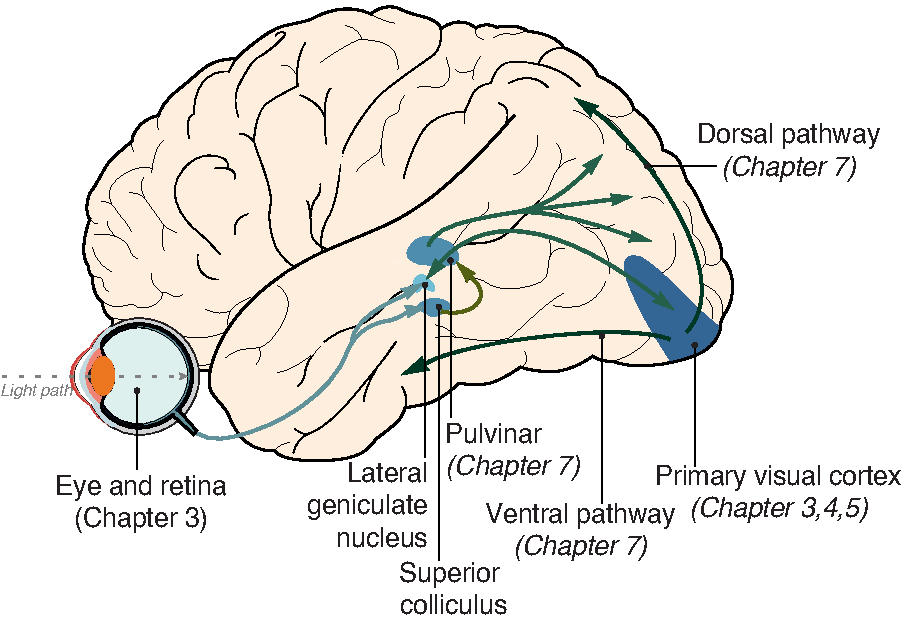
\includegraphics[width=.9\textwidth]{fig/chap2_fig_visual_system.pdf}
\caption[A schematic overview of the visual system.]{A schematic overview of the visual system. Electromagnetic waves (photons) are transduced in the retina into binary neural activity (spikes), which are then transmitted through the optic nerve to the \gls{LGN}, and then to \gls{V1}, before being processed by further cortical areas. The present chapter introduces general notions to the visual system, with specific part discussed further in the chapters indicated here in \textit{italics}. Figure adapted from~\cite{kandel2000principles}.}
\label{fig_chap2_vision_overview}
\end{figure}

Vision relies on a sophisticated bilateral sensing organ, the eye, which can be likened to an extraordinarily intricate adjustable-focus camera (Figure \ref{fig_chap2_vision_eye_retina}). Light enters the eye via the cornea, continues through the transparent aqueous humor, and proceeds through the pupil, which the opening of an aperture-regulating diaphragm, the iris. The focusing of the light source is then performed by the biconvex lens of the crystalline, which is dynamically adjusted by tiny muscles that modify the focal length. The nervous system thus possesses control over these components, enabling visual signals to act as feedback for adjusting the eye's optical characteristics in a closed-loop system~\cite{fernandez2001closed}.

\begin{figure}[h!tbp]
\vspace{0.5cm}
\centering
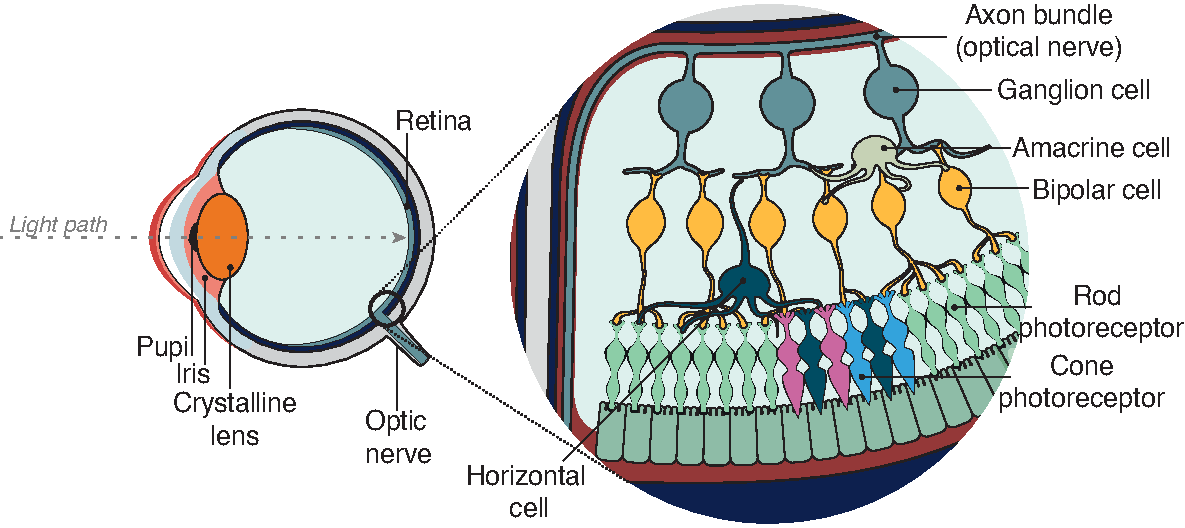
\includegraphics[width=.9\textwidth]{fig/chap2_fig_retina.pdf}
\caption[Illustration of the eye and retina.]{Illustration of the eye and retina. Adapted from~\cite{holmes2018reconstructing}.}
\label{fig_chap2_vision_eye_retina}
\end{figure}
Only then does light reach the photosensitive surface situated at the rear of the eye: the retina. Interestingly, the light must also traverse the full depth of the retina before being actually captured, as the light-sensitive part of the retina lies in its depth rather than on its surface. This propagation through the retina disperses the light, resulting in a somewhat lower-quality image. However, this is compensated for by a particular type of cell that channels light~\cite{newman1996muller}, but also contributes to a space-efficient design~\cite{kroger2009space}. 
A unique feature resulting from this architecture is that the axons from the retina's neurons must exit through the posterior section of the eye, and in doing so, must traverse the retinal depth in its entirety in some place. This is done in a single location, known as a "scotoma", which is thus devoid of photoreceptors and lacks direct visual input. However, this visual gap is seamlessly filled in, rendering it unnoticed in our conscious experience~\cite{rohrschneider2004determination}.

Aside to this particular design, the retina is a remarkably effective sensor. Specialized cells, the photoreceptors, convert light into electrical signals via a photosensitive molecule named retinal. These photoreceptors cells come in two varieties: cones, which cover different portions of the visible spectrum, providing important color visual information that we shall not be concerned with in this thesis~\cite{gegenfurtner2003color}; and rods, which are useful in situations with low light intensity. These photoreceptors are distributed in a particular pattern throughout the retina, where the densest concentration of cones is found near the center of the visual field, in the "fovea". This means that in order to obtain the maximum density of light-sensing cells, and thus extract the maximum amount of visual information, the eye must hover in to points of interests~\cite{friston2012perceptions}, which occurs about every hundred of milliseconds in primates~\cite{ibbotson2011visual}. 

The signals from these two types of cells are conveyed in a two-stream parallel process: either to the bipolar cells, carrying feedforward signal processing~\cite{ghosh2004types}, or to the horizontal cells, which carry out lateral integration in the retina, a process that contributes to enhancements in contrast~\cite{masland2012neuronal} and the early recognition of motion~\cite{olveczky2003segregation, liu2021predictive}. The output of this whole early sensory processing is carried out by retinal ganglion cells, whose axons are bundled into the optic nerve and sent deeper into the brain.

This nerve eventually reaches the brain's central hub, the thalamus. In the particular case of the optic nerve, the dedicated thalamus nucleus that receives inputs from the optic nerve is the \gls{LGN}, which is located in the posterior part of the thalamus. The wiring from the retina to the \gls{LGN} is not straightforward, in the literal sense, as part of both eyes' field of view will cross each other over before reaching the thalamus, likely due to an evolutionary twist of the body plan that also resulted in similar decussation (crossing of the middle plane) in the spine~~\cite{kinsbourne2013somatic, larsson2013optic}.
To simply label the thalamus as a relay would be a major oversimplification~\cite{sherman2007thalamus}, as the inputs from the retina to the thalamus represent less than one tenth of the synapses~\cite{ghodrati2017towards}, which might translate into even less than one tenth of actual functional impact~\cite{briggs2011corticogeniculate}.

%Different types of retinal ganglion cells are partitioned into layers within the thalamus of primates, including humans, several types of \gls{LGN} cells convey different kinds of visual information: P cells (Parvocellular), M cells (Magnocellular), and K cells (Koniocellular). P cells are relatively small, and convey information about fine details and color ; M cells are relatively large and convey information about motion and rapid temporal changes ; K cells are less understood, but seem to be linked in the integration of visual and non-visual information~\cite{kaplan2004m}. 

\begin{figure}[h!tbp]
\vspace{0.5cm}
\centering
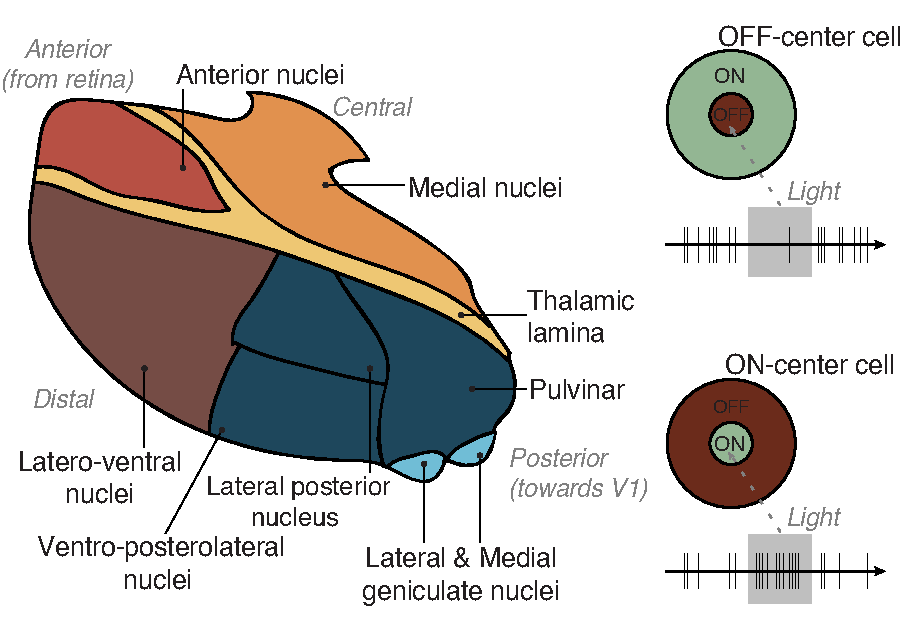
\includegraphics[width=.9\textwidth]{fig/chap2_fig_lgn.pdf}
\caption[Illustration of the \gls{LGN} and nearby thalamic nuclei.]{(left) Anatomy of the \gls{LGN} and nearby thalamic nuclei. Afferences from the optic nerve arrive at the \gls{LGN}. The superior colliculus, located near the cerebellum, is not represented. (right) Illustration of the ON/OFF activation of neurons in the \gls{LGN}.}
\label{fig_chap2_vision_lgn}
\end{figure}

Effectively, the \gls{LGN} acts as the preliminary stage for information consolidation, characterized by cells that perform an ON/OFF transformation of visual input, inherited from the mode of action of retinal ganglion cells (Figure \ref{fig_chap2_vision_lgn}). ON-center cells are triggered by an increase in light intensity within the central portion of their responsive visual field, known as the "receptive field". Conversely, they are deactivated by an increase in light intensity at the periphery of their receptive field. OFF-center cells function in the opposite manner. This shift signifies the transition from encoding unipolar light intensity in the early retina to bipolar light intensity in the thalamus, a crucial transformation for encoding contrast, which paves the way for encoding complex features in the cortex. 

Throughout this thesis, this notion of "receptive fields" (mostly in \gls{V1}) will be central to the subject of study. It is thus worth to define it clearly here, and for that, we will follow its textbook definition as the region in the sensory space in which a stimulus modulates the activity of a neuron. For Sir Charles Sherrington, who coined this term, a receptive field was exemplified by the skin area that, when stimulated, modulated the activity of scratch reflex neurons in canines~\cite{sherrington1906observations}. In our context, a receptive field will always pertain to the spatial configuration of a visual stimulus that modulates the activity of a given neuron in \gls{V1}.

Before we progress to our ultimate stop, \gls{V1}, it's important to recognize the existence of what are referred to as "non-canonical" pathways from the retina. The superior colliculus, for example, constitutes about $10\%$ of the visual output of the retina in primates, though this proportion is increased to $50\%$ for the cat~\cite{orban2012neuronal}. Similarly, the pulvinar nucleus of the thalamus, while only briefly mentioned here, warrants major discussion in the introduction to chapter 7, as it plays an integrative role among various cortical areas while also integrating inputs from the retina~\cite{casanova2004functions}.  



\subsubsection{The neurobiology of vision \textit{intra} V1}
Following this five-page overview of precortical vision stages, we now shift our focus to the primary subject of this thesis: the primary visual cortex, \gls{V1}. Located in the most posterior region of the brain, the occipital lobe, it is also known as the striate cortex, due to the presence of the line of Gennari~\cite{glickstein1984francesco}, a massive bundle of axons originating from the \gls{LGN} that forms a stripe that can be observed with the naked eye.

\begin{figure}[h!tbp]
\vspace{0.5cm}
\centering
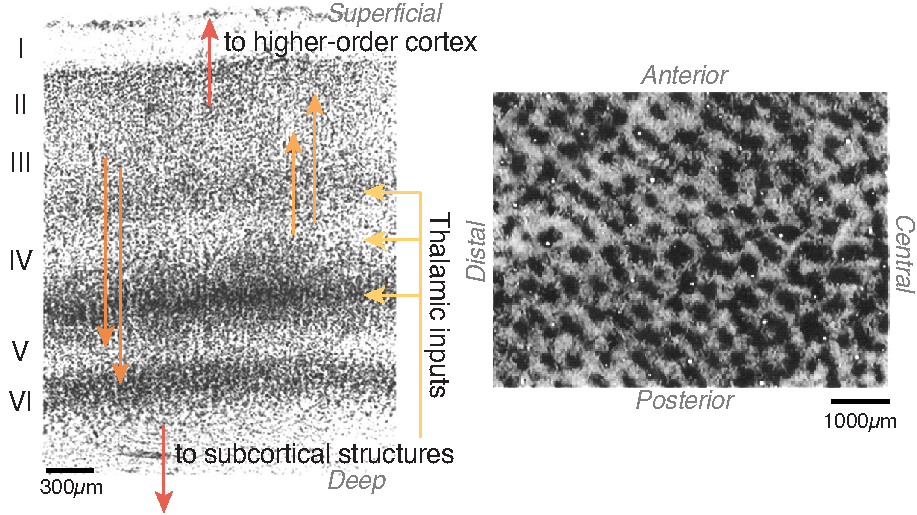
\includegraphics[width=.9\textwidth]{fig/chap2_fig_V1.pdf}
\caption[Primary visual cortex's anatomy.]{Primary visual cortex anatomy. (left) Nissl staining showing the vertical organization of macaque \gls{V1}, adapted from~\cite{schmolesky2011primary}. (right) Cytochrome oxydase staining, reflecting the horizontal organization of the thalamic inputs~\cite{takahata2016does}, adapted from~\cite{murphy1998spacing}.}
\label{fig_chap2_vision_V1}
\end{figure}

In terms of anatomy, like all non-motor cortices~\cite{shipp2013reflections}, \gls{V1} is composed of six layers. Despite ongoing debates surrounding the concept~\cite{horton2005cortical}, the "canonical" circuitry of this layered cortex suggests that visual information enters from the \gls{LGN} into the IVth cortical layer, is transported to layers II and III, and subsequently reaches layers V and VI~\cite{binzegger2004quantitative,douglas2004neuronal}. As we will see later in this introduction, this seemingly simplistic anatomical description is highly beneficial, as this pattern of connectivity is replicated across the whole cortex and can be thus mapped to general computations~\cite{douglas1989canonical, bastos2012canonical}. Organized orthogonally with respect to the cortical surface, this pattern establishes what is often referred to as a "cortical microcolumn.". Depending on the anatomist and the definition, its diameter fluctuates between 200 and 800 µm~\cite{mountcastle1997columnar}. Beyond this local anatomy, one should also note that layers II and III extend sizeable "lateral" axons, forming a "horizontal" circuitry~\cite{angelucci2006contribution,chavane2011lateral} that interconnects multiple similar microcolumns.

One can then naturally inquire about the functionality of these aforementioned circuit motifs. The main functional description of \gls{V1} can be traced back to a seminal study by Hubel and Wiesel, who conducted recordings from individual neurons in this area and discovered neural responses elicited for light bar of specific orientation~\cite{hubel1959receptive, hubel1962receptive}. Functionally, this feature expands upon the ON/OFF structure found in the \gls{LGN}, but incorporates a spatial layout that is lengthened, and thus appropriate for detecting edges in the visual field. Two distinct classes of cells demonstrate this "orientation selectivity": simple and complex cells. Simple cells, aptly named, react to edges of various orientations, and can be thought of as the convergence of many \gls{LGN} cells. Complex cells, on the other hand, exhibit overlapping ON and OFF fields and some degree of spatial invariance, and can be conceptually understood as a hierarchical~\cite{hubel1962receptive} (or lateral~\cite{chance1999complex}) convergence of several simple cells~\cite{boutin2022pooling}. Coherently, the majority of simple cells are found in layer IV and VI, whilst complex cells tend to be confined to layers II and III~\cite{payne2001cat}.
At the broader (mesoscale) level, the selectivity to orientation is arranged into maps of preferred orientation~\cite{grinvald1986functional}, where adjacent cells encode different orientations. This arrangement can be seen as essentially a competition for the best representation of objects that are present at a specific point within the visual field~\cite{kastner2001neural}. For a further detailed account of orientation selectivity, we refer the reader to chapter 4's introduction.

\begin{figure}[h!tbp]
\vspace{0.5cm}
\centering
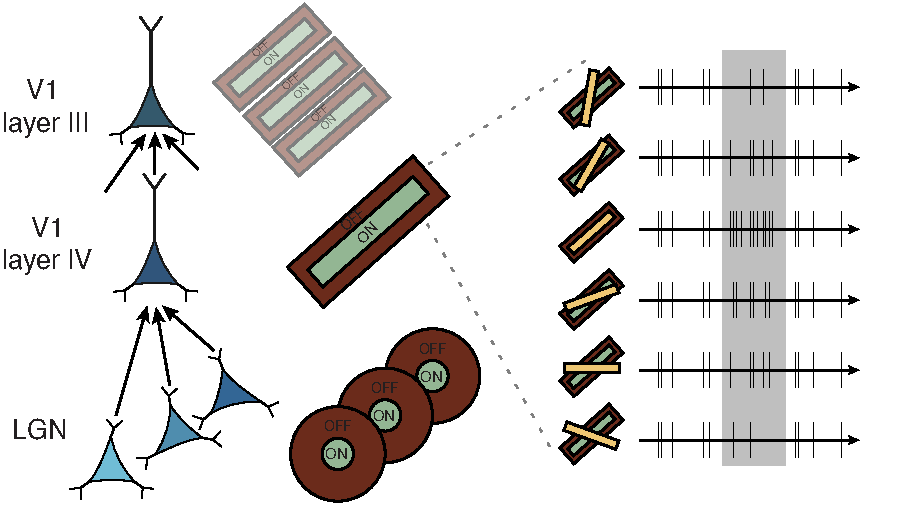
\includegraphics[width=.9\textwidth]{fig/chap2_fig_V1_ori_selec.pdf}
\caption[Illustration of orientation selectivity in V1.]{Illustration of orientation selectivity in \gls{V1}, as a hierarchical model~\cite{hubel1962receptive} from unoriented \gls{LGN} neurons, to simple then complex \gls{V1} cells.}
\label{fig_chap2_vision_V1_ori_selec}
\end{figure}

While orientation selectivity is the core concern of this thesis, there exists also other visual properties encoded by \gls{V1}. A non-exhaustive list would contain the spatial frequency~\cite{tolhurst1981variety}, referring to the scale of a specific feature and to its repeated size in the visual field. Like orientation, spatial frequency is also represented in a spatial frequency map that seems to be independent of orientation selective maps~\cite{issa2000spatial}. Possibly the most critical visual property encoded by \gls{V1} asides orientation is visual eccentricity and elevation, i.e. the spatial localization of visual stimuli~\cite{wandell2007visual}. In primates, there is a specific and highly ordered mapping of the visual field onto the topology of \gls{V1} that is well-captured by a mathematical "log-polar" transformation~\cite{traver2010review}. The closer a particular region of \gls{V1} is to the midline border, the more centrally located within the fovea that region's corresponding visual field will be. This precise arrangement allows for the efficient processing of visual information, enabling dense dedicated regions in the retina to have similar dense dedicated processing region in \gls{V1}. This density spreads throughout the cortical area, thereby providing an "over-representation" of the central portion of the visual field (encoded by the foveal region), with respect to its peripheral portions~\cite{jeremie2023retinotopy}.

V1 is not solely influenced by feedforward and local lateral interactions. It is, in fact, an integral component of a meticulously organized hierarchical network~\cite{scannell1995analysis}. \gls{V1} extends projections to various "extrastriate" cortical areas, such as V2, V4, and IT, as well as to subcortical areas, such as the pulvinar. While the role of these pathways will be occasionally referenced throughout the articles compiled in this thesis, they are not a primary focus of ours, and will be thus reserved for their respective dedicated chapters (4 and 7).

As these chapters also deal with neural recordings gathered from anesthetized cats, one should note a few differences between theirs and the primates' visual systems.
While both possess a primary visual cortex, or \gls{V1}, primates have a greater number of color-detecting cones leading to better color perception, whereas cats have more rods~\cite{sterling1983microcircuitry, kolb1984neural} aiding their low-light vision and 3D motion estimations, due to their nocturnal niche. \\
The main difference that concerns us however lies in \gls{V1}. At the macroscale, the cat's \gls{V1} is composed of Broadmann areas 17 and 18, instead of a single area in primate. Area 17, which was the targeted recording region in chapter 4, receives signals from the cat's equivalent of primate \gls{LGN}'s P cells (X in cats, concerned with fine details) and M cells (Y in cat, concerned with motion information)~\cite{stone1973projection}. Area 18 on the other hand mainly receives axons from the Y cells~\cite{payne2001cat}. 
At the mesoscale, likely to their respective cortical sizes and number of neurons~\cite{kaschube2014neural}, the cortical maps in \gls{V1} have different shapes~\cite{schmidt2021punctuated}, but both species show columnar organization, unlike rodents~\cite{kaas2022escaping}. 
At the microscale, it seems that the general pattern of connectivity is similar, but with difference in specificities of laminar connections, namely from layer IV to III~\cite{lund1979anatomical}. 
The reason for this seemingly mixed model usage in the literature is partly accounted by the fact that cats have been the main historical model under study. As such, the wealth of 60 years of data gathered in the cat visual system, combined with the complexity involved in primate experiments, still makes them highly relevant to vision research. 



\subsubsection{The statistics of natural and naturalistic visual inputs}
Having introduced the basic notions of orientation selectivity and the neurobiological substrates of vision, we can now turn back to the goal we had set in the first place: provide a computational account of vision.

Understanding what vision does, without understanding what type of input vision must process, would be a daunting task. Vision is tasked with processing the complexity and richness of the images that form our everyday perceptual experiences, colloquially known as "natural images". These images, despite their immense diversity and complexity, are all governed by the same physical laws~\cite{stevens1974patterns}, leading to observable statistical regularities. This proves to be an essential feature, given that the neural activity required to process these images is energetically costly~\cite{laughlin1998metabolic}. Further, any sensory processing is under the constraint of extreme time efficiency required for the survival of our organisms~\cite{thorpe1996speed, kirchner2006ultra}.
Horace Barlow~\cite{barlow1961possible} posited that up to \gls{V1}, the purpose of vision is to eliminate such statistically redundant data, thereby optimizing energy usage and speeding up computations. This perspective, often referred to as efficient coding~\cite{olshausen1996natural} allows providing a quantitative description of sensory systems with respect to their environments~\cite{simoncelli2001natural}.

\begin{figure}[h!tbp]
\vspace{0.25cm}
\centering
\includegraphics[width=.9\textwidth]{fig/chap2_fig_natimg.pdf}
\caption[An example of natural image statistics.]{(top) An example of natural image, Marseille's "calanques"~\cite{ladret2023cortical}, with local distribution of orientations shown on the right for multiple patches. (bottom) The statistics of this image, from left to right: distribution of luminance, cumulative luminance frequency, $1/f^2$ Fourier power spectrum.}
\label{fig_chap2_stats_natimg}
\end{figure}

We will here overview such quantitative accounts to get a better sense of the structure of the visual world. Such structure will eventually lead us to a formulation of vision as a variance-bound problem. Fundamentally, vision concerns itself with the perception of light patterns and is, therefore, inherently constrained by the statistical characteristics of light intensity. Most, but not all, (namely in terms of contrast) of these light intensity statistics are primarily the problem of the retina~\cite{barlow1956retinal}. Even though they are not the focal point of this thesis, it is crucial to acknowledge them, as the statistical regularities of vision are hierarchical, and thus the ones of light patterns provide substantial insight into the higher-order statistics of vision. In terms of pure lighting intensity, the distribution of natural images follows a Gaussian structure~\cite{laughlin1981simple}. In line with Barlow's efficient coding hypothesis~\cite{barlow1961possible}, the cumulative probabilities of such distribution actually mirrors the response to contrast in the retina's~\cite{naka1966s, laughlin1981simple}. This suggests an optimal tuning of the retina to respond to the intensity of light, underlying the interplay between the statistical properties of the natural environment and the sensory systems evolved to process them. This same kind of input/system "echo" will be further described in chapter 3.

The spatial organization of light intensity presents further statistical regularities that can help our posing of the vision problem. If one is to read this manuscript in a laboratory, an intuitive observation that can be had from gazing just about anywhere in a modern monochrome office space is the strong correlation in light intensity between neighboring locations. The same is also true, to a lesser extent, in natural images. Applying a Fourier transform to analyze such an image in the frequency domain, the correlation in intensity between nearby pixels becomes apparent in the form of a concentration of power in the lower frequencies of the spectrum. These low frequencies correspond to larger, more global structures, while the less powerful higher frequencies denote smaller, localized variations. This relationship is captured by a $1/f^x$ relationship characteristic observed in natural images, where often $x \approx 2$~\cite{tolhurst1992amplitude}.

This leads us to the notion that natural images also contain useful statistical regularities for higher-order features, like orientation. A noteworthy empirical demonstration by Bruno Olshausen and David Field~\cite{olshausen1997sparse, olshausen1996emergence} reveals that when trained on natural images, reconstructive models will naturally yield oriented filters that are strikingly (and quantitatively) similar to those of \gls{V1}. The statistics of such edges even enables prediction of high-level features in an efficient and unsupervised manner~\cite{perrinet2015edge}, possibly priming many downstream computations.
In orientation space, this representation is highly sparse, with only a selected few orientations required at each spatial localization to reconstruct an image~\cite{field1987relations}. In feature space, however, the distribution of oriented features in natural images remain underexplored in existing literature, with a few exceptions. Mathematically, a single image embodies infinite uncertainty, with an uncharacterized distribution featuring high activations around the horizontal and vertical axes~\cite{hansen2004horizontal}. In chapter 3, we propose a more detailed exploration of the statistical structure of these oriented features, with the prevailing assumption being that the distribution follows a Gaussian pattern in orientation space.

This final note gives us an opportunity to keep statistical regularities in mind when talking about vision, whilst also getting essentially rid of natural images. While we briefly detailed their useful statistical regularities here, they are mostly just poised with intractable complexity~\cite{gauvrit2014natural, rust2005praise}. Because of this, and because of historical technical complexities, vision has mainly experimented with artificial stimuli since its inception $60$ years ago. This has given investigations a methodology that affords a degree of parametric control over the multifaceted system of vision~\cite{priebe2016mechanisms}, but has had the unfortunate drawback of not eliciting the same types of activation as natural images~\cite{fiser2004small, yoshida2020natural, baudot2013animation}. 
This enduring debate between the use of "natural" versus "artificial" stimuli leads us to a using a satisfying compromise in this thesis: the "naturalistic" stimuli. Such experimental approach aims to strike a balance between replicating the statistical properties of natural scenes and maintaining the experimental control offered by fully artificial stimuli, thereby providing an optimal platform for investigating the intricacies of vision.

\begin{figure}[h!tbp]
\vspace{0.25cm}
\centering
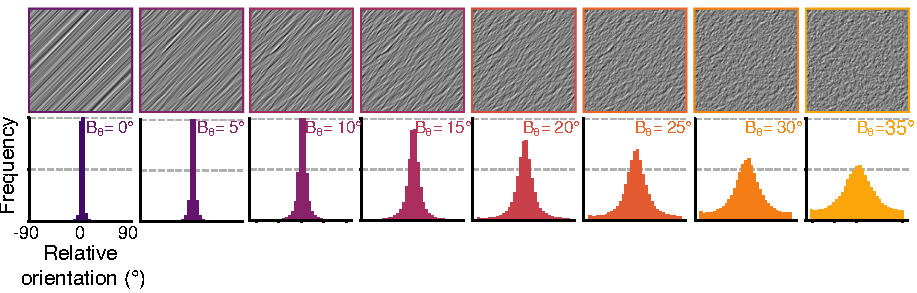
\includegraphics[width=.9\textwidth]{fig/chap2_fig_motionclouds.pdf}
\caption[An example of Motion Clouds.]{An example of Motion Clouds, with increasing orientation variance from left to right, and associated orientation distributions.}
\label{fig_chap2_stats_mc}
\end{figure}

Here, we will focus on the case of Motion Clouds, generative model-based stimuli~\cite{leon2012motion} which allow for fine parameterized control over a naturalistic stimuli~\cite{vacher2015biologically}, which is a desirable trait when probing sensory systems under realistic conditions~\cite{rust2005praise}. They are mathematically defined as band-pass filtered white noise stimuli, whose filters in Fourier space are defined as a parameterized distribution in a given perceptual axis (here, only orientation). 
Thus, the Motion Clouds presently used are fully characterized by their mean orientation and their orientation variance, such that a given stimulus $S$ can be defined as:

\begin{equation}
    \text{S} = \mathcal{F}^{-1} (O(\theta, B_{\theta}))
\end{equation}

where $\mathcal{F}$ is the Fourier transform and $O$ the orientation envelope, characterized by its mean orientation $\theta$ and its orientation bandwidth $B_\theta$. For $B_\theta < 45.0$°, a good approximation is $B_\theta = 1/\sqrt{\kappa}$, where $\kappa$ is the concentration parameter of a von Mises distribution (see below), and hence approximates the standard deviation~\cite{swindale1998orientation}. It thus serves as a measure of the orientation variability in the pattern, and as such, we will use the term "variance" to describe it throughout the thesis.
The orientation envelope is a von Mises distribution:
\begin{equation}\label{eq_orientation_mc}
O(\theta, B_{\theta}) = 
\exp 
\left\{
\frac{\cos (2 (\theta_f - \theta)) }
{4 \cdot B_{\theta}^2}
\right\}
\end{equation}
where $\theta_f$ is the angle of the frequency components of the envelope in the Fourier plane, which controls the spatial frequency parameters of the stimuli. For the range of values of $B_\theta$ considered in the present thesis, the orientation envelope approximates a Gaussian distribution and $B_\theta$ is thus a measure of the variance of the orientation content of the stimuli that follows a naturalistic distribution, as highlighted in chapters 3, 4 and 5. 

Such stimuli offer three advantages over both simple grating-like stimuli and complex natural images. First, they enable fine control of mean orientation, controlled by $\theta$, and its variance, controlled by $B_\theta$. This thus allows to reproduce natural images' oriented content, solely in terms of orientation distributions. Second, as they are stationary in the spatial domain, they only probe orientation space, excluding any second-order information exploitable by the visual cortex~\cite{johnson2004first}. Third, by conforming to natural images' $1/f^2$ power spectrum distribution~\cite{field1987relations}, they attain a desirable balance between controllability and naturalness~\cite{rust2005praise}. The combination of these traits allowed Motion Clouds to be successful in describing the perceptual integration of the human visual system~\cite{simoncini2012more}, the dynamical computations of retina~\cite{ravello2019speed}, and the dynamics of naturalistic perception in \gls{V1}~\cite{vacher2017synthese}. Controlling a naturalistic stimulus confers a significant benefit here, namely in allowing us to control the variance of these distributions, whose role in vision we will now explore.



\subsubsection{Variance in vision}
Herman von Helmholtz, in his treatise of physiological optics~\cite{helmholtz1925treatise}, gave a pinpoint accurate description of variance in sensory perception:
\begin{displayquote}
	“Given that the world we live in is loaded with statistical noise, [$\approx$ variance] expectations must be represented as part of the brain’s models.”
\end{displayquote}

Sources of variance are plentiful in vision (Figure \ref{fig_chap2_variance_psychophysics}). Well-known optical illusions demonstrate how an object can seem brighter than it actually is, when light intensity is juxtaposed against a dark background. Obstruction patterns lead us to inaccurately fill in parts of the visual field. Motion can blur our perception. Here, our primary interest lies in the orientation variance and its effect on vision, a sub-field that has been extensively explored psychophysically, yet remains relatively uncharted in terms of electrophysiological investigations.

\begin{figure}
\vspace{-0.25cm}
\centering
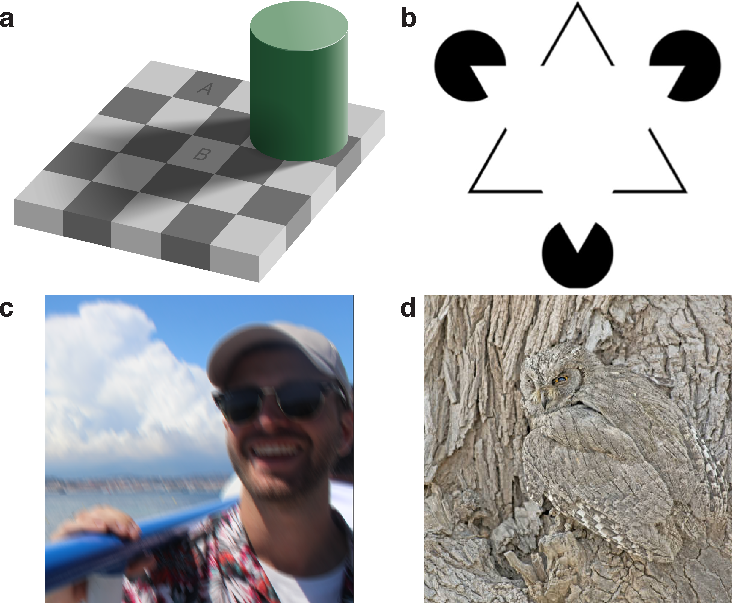
\includegraphics[width=.75\textwidth]{fig/chap2_fig_visionvariance.pdf}
\caption[Example of visual uncertainties.]{Example of visual uncertainties, on: (a) contrast, (b) obstruction, (c)  motion blur, (d) orientation (picture taken by \href{https://www.flickr.com/photos/noorhussain}{Noor Hussain}).}
\label{fig_chap2_variance_psychophysics}
\end{figure}

In psychophysics, variance is often interchangeably used with the term 'uncertainty'~\cite{szeliski1990bayesian}. In the context of orientation, the term 'bandwidth' is also often used, for historical reason~\cite{snowden1992orientation}, as studying a broadband signal in orientation domain is straightforward, and creating such a signal by blending point sources of orientation to generate a distribution is even simpler. In statistical term, one can also use inverse variance ($1/\sigma$) and its squared term, the precision ($1/\sigma^2$). Under Gaussian approximation, such as in chapter 3 and 4 (see also Equation~\ref{eq_orientation_mc}), bandwidth approximates variance, and both can be linked to inverse variance and precision through their straightforward mathematical relationship. Uncertainty, when used in this manuscript, will also refer to the notion of a "broader" distribution of features (often, of orientations). One could nonetheless be "certain" of a given large "variance", for example, by asking a human subject to judge the degree of variance of a given texture. That specific meaning will not be used in this manuscript (see for example~\cite{barthelme2009evaluation,geurts2021reported,sanchez2023action}), and we will refer to inverse variance and variance when describing the computations at play here.

The general study of orientation variance can be traced back to parametric texture generation, starting with Bela Julesz work on "textons"~\cite{julesz1981textons}. These simple oriented elements were shown to human subjects, and shown to take an increasingly great amount of time to process as their complexity (i.e. variance in orientation space) increases~\cite{julesz1983human}.
Under different texture synthesis algorithms and experimental paradigms, this observation has been replicated a number of time, showing that the impact of increasing variance on orientation detection is rather intuitive: as variance rises, performance deteriorates~\cite{phillips1984orientation,heeley1989width,heeley1998influence}. This is a non-linear effect~\cite{heeley1998influence} that works similarly to contrast response curve. Computationally, it is well accounted for by models of recurrent cortical activity~\cite{keeble1995detection,beaudot2006orientation}, and more specifically the result from the competition among multiple orientation detectors~\cite{ringach2002orientation}.

This is however not a mere passive influence, but an active mechanism, accounted for by human observers~\cite{barthelme2009evaluation}. This behavior aligns with Bayesian models of perception, which, as we will discuss in the upcoming algorithmic section of the introduction, is of central importance for our work. Briefly, a Bayesian account of perception implies an active encoding of variance in the brain, granting access to this information for decision-making~\cite{geurts2022subjective}. For instance, let us imagine an observer walking through a forest and hearing leaves rustling. If one's vision is clear, and one spots a squirrel, they'd likely carry on without concern. However, if their vision is obstructed by dense bushes (creating an increased orientation variance), they'd likely rely more heavily on their internal priors, which in most instances, would dictate a cautious retreat. Vision does not work as passive acceptance of uncertain input, but rather, requires our brain to cross-reference what it sees with a prior model of the world.

Despite the convergence psychophysical accounts and theoretical requirements, there is a significant gap in the literature on the implementation of variance computations in the brain~\cite{koblinger2021representations}. This discrepancy could be attributed to the complexities involved in applying parametric texture synthesis to probe the visual system, making electrophysiological investigations challenging. As this section of the introduction primarily focuses on the computational level, we direct the reader to the concluding part of the introduction for a detailed explanation of the implementational mechanisms of variance within the brain, and now turn our attention to describing the basic requirements for variance-based in computations.



\newpage 



\subsection{The algorithmic level: A probabilistic model of perception}
Marr's second level, the algorithmic level, is concerned with the operations that the system performs, and how these are organized to realize the computations described at the previous level. This section aims to describe probabilistic operations that can account for visual tasks, adopting an iterative approach to the problem of perception. We will follow the common formalism and mathematical development for this class of problem~\cite{bogacz2017tutorial}, framed with additional justifications of equations and examples fitted to the problem under study.

\subsubsection{A simple example of Bayesian Inference}
We start by considering a simplistic toy example in which an organism is tasked with inferring a single variable, the size of a food item denoted by $v$, based on a single observation, the light intensity denoted by $u$. The organism's sensory input is constrained, as ours, to be noisy~\cite{barlow1956retinal}, such that the true item size $v$ is normally distributed based on observations $u$. Given that light reflections are related to the surface of the object, let's consider a distribution with a mean true item size $g(v)$, where $g(v) = v^2$, and a variance based on noise on observations $\Sigma_u$. This is expressed as:

\begin{equation}\label{eq_proba_intro}
    p(u|v) = f(u;g(v), \Sigma_u) = \frac{1}{\sqrt{2\pi\Sigma_u}} exp{\frac{(u-g(v))^2}{2\Sigma_u}} 
\end{equation}

Given this probabilistic description of the input and the arguments previously stated in favor of vision as a probabilistic process, we shall also describe such organism as performing probabilistic inference. We thus consider that this organism has had the chance of encountering many food items in his life, and that it can implement prior expectation $p(v)$ about the size of the food item. This is also normally distributed, with mean $v_p$ and variance $\Sigma_p$:

\begin{equation}
p(v) = f (v; v_p, \varSigma_p) = \frac{1}{\sqrt{2\pi\Sigma_v}} \exp{\frac{(v-v_p)^2}{2\Sigma_p}}
\end{equation}

Given this framework, we can apply Bayes' theorem to compute an exact solution to the inference problem based on a single observation of light intensity, which is given by:

\begin{equation}
\label{eq_denominator}
p(v|u) = \frac{p(v)p(u|v)}{p(u)} = \frac{\frac{1}{\sqrt{2\pi\Sigma_p}} \exp{\frac{(v-v_p)^2}{2\Sigma_p}} \frac{1}{\sqrt{2\pi\Sigma_u}} \exp{\frac{(u-g(v))^2}{2\Sigma_u}}}{\int p(v) p(u|v)dv}
\end{equation}

The numerator term is simply the product of the prior and the likelihood described above. The normalization term, however, is more complex. It is the integral of all $p(v)p(u|v)$, which ensures that the posterior probabilities of $p(v|u)$ sum to $1$, but is too computationally intensive for a realistic system, as it would require sampling all possible configurations of the problem. This consideration is left to the implementational level of the introduction, and does not deter us presently from computing an exact solution using Bayes' theorem. This yields the graphical representation of integrating likelihood $p(u|v)$ and prior $p(v)$ into a posterior distribution $p(v|u)$. 

\begin{figure}[h!tbp]
\vspace{0.5cm}
\centering
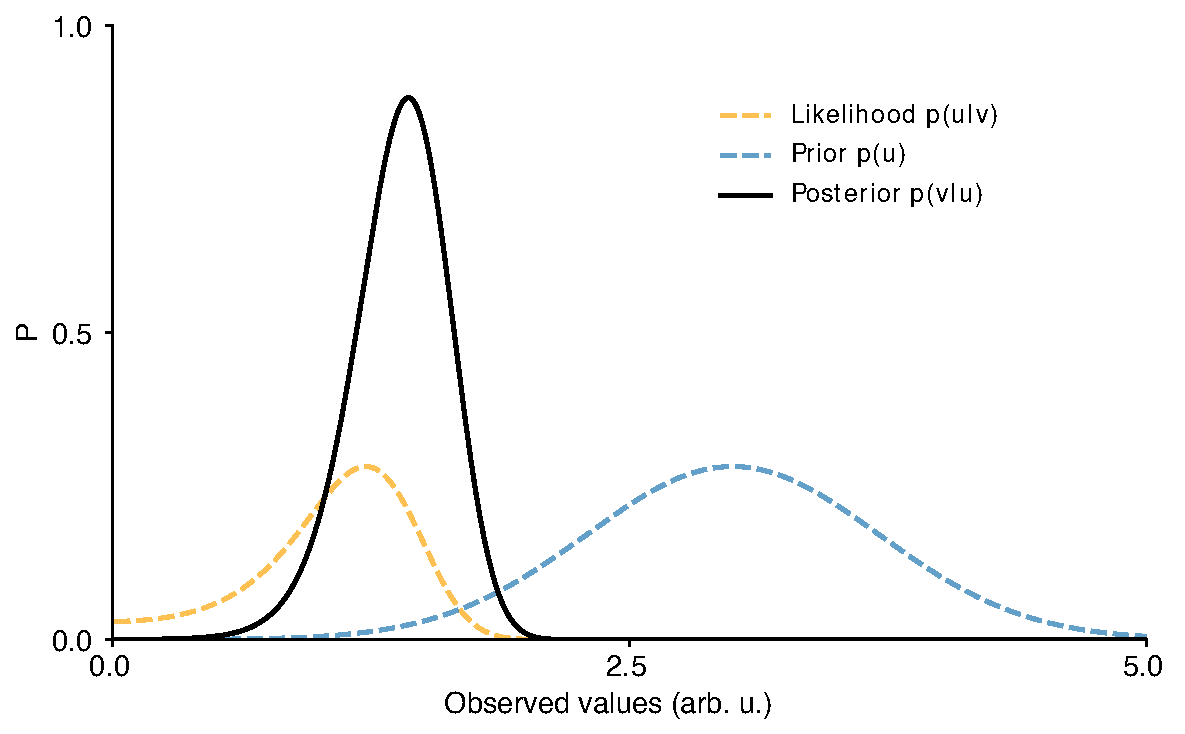
\includegraphics[width=.9\textwidth]{fig/chap2_fig_equi_proba.pdf}
\caption[A simple example of Bayesian integration.]{A simple example of Bayesian integration. Integrating observed (likelihood) and former (prior) distributions, with $\Sigma_u = \Sigma_p = 0.5$. The most likely value of $v$ lies between the two distributions.}
\label{fig_chap2_equi_proba}
\end{figure}

Through the representation of Figure \ref{fig_chap2_equi_proba}, one can notice how non-intuitive and non-linear Bayesian inference can be, even in such a simple example framed here. For the organism that must estimate $p(v|u)$, once the (input) likelihood $p(u|v)$ involved becomes a non-standard distribution, it becomes necessary to represent infinitely many $p(v|u)$ values for many possibles $v$, rather than first order statistics like mean and variance. As we've said, however, this would require infinitely too many computations for a biological system. Instead of computing the whole distribution, this organism could try to maximize the value of $p(v|u)$, in order to infer the most likely value of $v$. This procedure is called \textit{maximum likelihood estimation} and involves sampling a posterior distribution $p(\Phi | u)$ of the most likely size $\Phi$:

\begin{equation}
\label{eq_MLE}
p(\phi|u) = \frac{p(\phi)p(u|\phi)}{p(u)}
\end{equation}

As the denominator does not depend on $\Phi$, we focus on the numerator. We will denote its logarithm $F$, as it relates to the Free Energy described later:

\begin{equation}
     F = \ln  \left( p(\Phi) p(u|\Phi) \right) = \ln p(\Phi) + \ln p(u|\Phi)
\end{equation}

The natural logarithm having removed the exponential terms involved in Equation~\ref{eq_denominator}, we get: 
\begin{equation}
\label{eq_F}
  \begin{aligned}
    F & = \ln p(\Phi) + \ln p(u|\Phi) \\ 
      & =\ln \left( \frac{1}{\sqrt{2\pi\Sigma_p}} \exp{-\frac{(\Phi-v_p)^2}{2\Sigma_p}}\right) + \ln \left( \frac{1}{\sqrt{2\pi\Sigma_u}} \exp{-\frac{(u-g(\Phi))^2}{2\Sigma_u}} \right) \\
      & = \ln \left( \frac{1}{\sqrt{2\pi\Sigma_p}} \right) + \ln \left(\exp{-\frac{(\Phi-v_p)^2}{2\Sigma_p}} \right) + 
            \ln \left( \frac{1}{\sqrt{2\pi\Sigma_u}} \right) + \ln \left(\exp{-\frac{(u-g(\Phi))^2}{2\Sigma_u}} \right) \\
      & = \ln \left( \frac{1}{\sqrt{2\pi}} \right) - \frac{1}{2} \ln \Sigma_p- \frac{(\Phi-v_p)^2}{2\Sigma_p} + 
            \ln \left( \frac{1}{\sqrt{2\pi}} \right) - \frac{1}{2} \ln \Sigma_u -  \frac{(u-g(\Phi))^2}{2\Sigma_u} \\ 
      & =  \frac{1}{2} \left( - \ln \Sigma_p - \frac{(\Phi - v_p)^2}{\Sigma_p}  - \ln \Sigma_u - \frac{(u - g(\Phi))^2}{\Sigma_u}\right) + C
  \end{aligned}
\end{equation}

Now, it is simpler to find the derivative of $F$ to look for a maximum value of our food estimate posterior distribution, we can compute the derivative of $F$ over $\Phi$ (as done in Appendix \ref{appendix_maths}), we get:

\begin{equation}
\label{eq_dF_dPhi}
    \frac{\delta F}{\delta \Phi} = \frac{(u-g(\Phi))}{\Sigma_u} g'(\Phi)  + \frac{(v_p-\Phi)}{\Sigma_p}  
\end{equation}
which endows our example organism with the ability to find the most likely value of the food item size $v$ by varying $\Phi$ with respect to the sign of the derivative. The first term of the equation drives the posterior distribution towards the likelihood, and the second one towards the prior, both of which are weighted by the inverse of their respective variance, $\Sigma$.
This equation is central to the remainder of this algorithmic part of the introduction, and really to this entire thesis, as it provides a mathematical role for variance in (visual) perception. It can be easily tied, in this form, to the Free Energy principle, introduced in the next section.



\subsubsection{Free Energy principle for variational inference}
The free energy principle allows both to understand how complex systems can model the most likely values of variables, as above, but also their distribution, as is the goal of this thesis. Briefly, this theory traces its roots to the work of Hermann von Helmhotz' unconscious inference~\cite{helmholtz1925treatise}, who was arguably the first physiologist to propose the notion that the mind construct a perception of the world through probabilistic inference. The idea of free energy in the brain gained popularity through the seminal works of Karl Friston~\cite{friston2006free, karl2012free, aguilera2022particular}, who also proposed its realization in the form of a neuroscience theory called predictive coding~\cite{friston2005theory, friston2009predictive}. In this section, we shall dive into the details of variational free energy, a specific formulation of free energy that will allow us to formulate general equations on which the rest of the thesis will rely.

In the text preceding Equation \ref{eq_MLE}, we mentioned that posterior distributions $p(v|u)$ can have complex shapes that mandate prohibitively dense sampling for many values of $u$. As an approximation to avoid this issue, we proposed the method of sampling solely the maximum of these distributions. However, it is beneficial to know the shape of the full distribution, namely for knowing the variance - and thus the reliability - of estimates~\cite{mansournia2016inverse}, as we wish to see in neurobiological systems in this thesis. An improved solution of maximum likelihood estimate is an alternative approach that involves the utilization of a "surrogate" distribution, in a process called variational inference~\cite{murphy2012machine}. This distribution, which we will refer to as $q(v)$, possesses a standard form that can be succinctly described by its mean and variance, unlike the distribution it surrogates in the first place.
To approximate our complex posterior $p(v|u)$ with $q(v)$, we need a metric of (dis)similarity between the two distributions. For probability distribution and without particular assumptions, the choice is naturally the \gls{KL} divergence, defined as: 

\begin{equation}
KL(q(v), p(v|u)) = \int{q(v) \ln \frac{q(v)}{p(v|u)} dv}
\end{equation}

This divergence, or distance, is not symmetric, meaning that the divergence from $p(v|u)$ to $q(v)$ is not the same as the divergence from $q(v)$ to $p(v|u)$. This characteristic makes it particularly suitable for our purpose, as it allows us to measure how much information is lost when we use the surrogate function $q(v)$ to approximate the original distribution $p(v|u)$. By minimizing the \gls{KL} divergence, we can ensure that our surrogate function is as close as possible to the original distribution, thereby providing a more accurate and efficient representation of the complex posterior distribution.

As is, this approach doesn't make things any easier, as we are still required to calculate the same normalization term as in Equation \ref{eq_denominator}, a barrier that led us to maximum likelihood estimate in the first place. This is where the concept of Free Energy proves to be immensely beneficial.
By definition, we already know that:

\begin{equation}
    p(v|u) = \frac{p(u, v)}{p(u)}
\end{equation}

which we can use into the equation of the \gls{KL} divergence as:

\begin{equation}
    \begin{aligned}
        KL(q(v), p(v|u)) & = \int{q(v) \ln \frac{q(v)}{p(v|u)} dv} \\ 
                        &= \int{q(v) \ln \frac{q(v)p(u)}{p(u,v)} dv} \\
                        &= \int{q(v) \ln \frac{q(v)}{p(u,v)} dv} + \int{q(v) \ln p(u) dv} \\
    \end{aligned}
\end{equation}

given that $q(v)$ is a probability distribution and sums up to $1$, we thus obtain:

\begin{equation}
    KL(q(v), p(v|u)) = \int{q(v) \ln \frac{q(v)}{p(u,v)} dv} + \ln p(u) \
\end{equation}

by defining the variational free energy as the negative of the term that is concerned with our surrogate distribution, we get:

\begin{equation}
\label{eq_free_energy_KL}
    \begin{aligned}
        F &= \int q(v) \ln \frac{p(u,v)}{q(v)} dv, \\
        KL (q(v), p(v|u)) &= -F + \ln p(u)
    \end{aligned}
\end{equation}

since only $F$ pertains to our surrogate distribution $q(v)$, the parameters of this function that minimize the divergence between $q(v)$ and the actual posterior $p(v|u)$ are the same as those that maximize $F$. Note that this $F$ denotes that variational free energy, that is, the free energy involved in this approximation process, and not the general free energy of the system. To obtain the best surrogate distribution to approximate the posterior, we can now simply maximize $-F$, which does not involve the complex computation of the normalization term. In the next section, this will also serve to introduce learning of parameters of models. As we shall soon see, such learning involves, intuitively, being wrong as rarely as possible in our inference process. In other term, we wish to minimize the surprise, as defined by Shannon~\cite{shannon1948mathematical}, associated with our predictions. Given Equation \ref{eq_free_energy_KL}:

\begin{equation}
\label{eq_lnpu}
    - \ln p(u) = F+ KL (q(v), p(v|u)) 
\end{equation}

As the \gls{KL} divergence is positive, $F$ can only be a lower bound of $\ln p(u)$. Maximizing the variational free energy $F$ thus minimizes surprise $\ln p(u)$, meaning that we improve the approximation of $q(v)$ and thus optimize our internal model using this simple framework.



\subsubsection{Prediction errors under the free energy principle}
As we are progressively moving from the algorithmic to the implementation level, our formulation of Bayesian inference under the Free Energy principle could use a reframing more related to neurobiology. In that sense, this section of introduction will tell us now how to formulate Bayesian inference in simpler terms, and second how to derive learning rules. 

Going back to Equation \ref{eq_dF_dPhi}, we showed that deriving the parameter $\Phi$ could be written as:

\begin{equation}
    \frac{\delta F}{\delta \Phi} = \frac{(u-g(\Phi))}{\Sigma_u} g'(\Phi)  + \frac{(v_p-\Phi)}{\Sigma_p}  
\end{equation}

we can now perform some helpful variable renaming, with the left-hand side of the equation becoming:

\begin{equation}
    \epsilon_p = \frac{(v_p-\Phi)}{\Sigma_p} 
\end{equation}

and the rest being:

\begin{equation}
    \epsilon_u = \frac{(u - g(\Phi))}{\Sigma_u}
\end{equation}

such that the derivative becomes:
\begin{equation}
\frac{\delta F}{\delta \Phi} = \epsilon_u  g'(\Phi)   + \epsilon_p 
\end{equation}

and the update rule of $\Phi$ to follow the gradient of $F$ is then:

\begin{equation}
    \dot{\Phi} = \epsilon_u  g'(\Phi) - \epsilon_p
\end{equation}

Both $\epsilon_p$ and $\epsilon_u$ measure the difference between a real and inferred value, and are thus both called prediction errors~\cite{friston2005theory} (hence the term predictive coding). The term $\epsilon_p$ is often referred to, in the literature~\cite{millidge2021predictive}, as the prediction error on the causes, and measures the difference between the inferred observation and the model's prior expectations. The term $\epsilon_u$, on the other hand, is called the prediction error on the states, and measures the difference between the observed value and the inferred value. In predictive coding, the goal of a model is to minimize both sources of prediction errors, and as such it needs a learning rule based on prediction errors. When looking for the point at which the system's prediction error become null, we get the stable point of $\epsilon_p$:

\begin{equation}
    \begin{aligned}
        \epsilon_p &= \frac{\Phi - v_p}{\Sigma_p} \\
        \Sigma_p\epsilon_p &= \Phi - v_p \\
        \Phi - v_p - \Sigma_p\epsilon_p &= 0 
    \end{aligned}
\end{equation}

and the one of $\epsilon_u$:

\begin{equation}
    \begin{aligned}
        \epsilon_u &= \frac{u - g(\Phi)}{\Sigma_u} \\
        \Sigma_u\epsilon_u &= u - g(\Phi)\\
         u - g(\phi) - \varSigma_u \varepsilon_u &= 0
    \end{aligned}
\end{equation}

And thus the dynamics of a system that seeks to minimize its prediction errors can be described as: 

\begin{equation}
\begin{aligned}
\dot{\varepsilon_p} &= \phi - v_p - \varSigma_p \varepsilon_p  \\
\dot{\varepsilon_u} &= u - g(\phi) - \varSigma_u \varepsilon_u  \\
\end{aligned}
\end{equation}

This is however not an ideal description, because it assumes the rest of the parameters of the system $v_p, \Sigma_p, \Sigma_u$ are constrained. It becomes even more inconvenient in a thesis about the implementation of dynamical computations on $\Sigma$ parameters. This is where the free energy principle becomes extremely useful, as it ascribes a goal to the model: modifying parameters such that visual input $u$ becomes the least surprising. As described in Equation \ref{eq_denominator}, this is a term that involves the computation of a complex integral, but its natural logarithm can be more easily computed as in Equation \ref{eq_lnpu}, and even more so with $F$ defined in Equation \ref{eq_F}:

\begin{equation}
\begin{aligned}
    \ln p(u) & = F+ KL (q(v), p(v|u)) \\
            & = \frac{1}{2} \left[ - \ln \Sigma_p - \frac{(\Phi - v_p)^2}{\Sigma_p}  - \ln \Sigma_u - \frac{(u - g(\Phi))^2}{\Sigma_u}\right] + C + KL (q(v), p(v|u))
\end{aligned}
\end{equation}

as the \gls{KL} divergence is a strictly positive term that forms a lower bound on surprise, we will include it in the constant $C$ term for simplicity's sake. Following the (lenghty) derivations in Appendix \ref{appendix_maths} of $F$ over $v_p, \Sigma_p, \Sigma_u$, we get the following dynamics of our inference model:

\begin{equation}
\label{eq_df_derror}
    \begin{aligned}
    \frac{\delta F}{\delta v_p} &= \frac{\Phi - v_p}{{\Sigma_p}} \\
    \frac{\delta F}{\delta \Sigma_p} &= \frac{1}{2} \left[ \frac{(\Phi - v_p)^2}{{\Sigma_p^2}} - \frac{1}{{\Sigma_p}} \right] \\
    \frac{\delta F}{\delta \Sigma_u} &=  \frac{1}{2} \left[ \frac{(u - g(\Phi))^2}{{\Sigma_u^2}} - \frac{1}{{\Sigma_u}} \right]
    \end{aligned}
\end{equation}

by re-expressing these equations using the definition of prediction error as before, we get:

\begin{equation}
\label{eq_df_derror_final}
    \begin{aligned}
    \frac{\delta F}{\delta v_p} &= \frac{\Phi - v_p}{{\Sigma_p}} = \epsilon_p \\
    \frac{\delta F}{\delta \Sigma_p} &= \frac{1}{2} \left[ \frac{(\Phi - v_p)^2}{{\Sigma_p^2}} - \frac{1}{{\Sigma_p}} \right]  = \frac{1}{2} \left(\epsilon_p^2 - {\Sigma_p^{-1}} \right) \\
    \frac{\delta F}{\delta \Sigma_u} &=  \frac{1}{2} \left[ \frac{(u - g(\Phi))^2}{{\Sigma_u^2}} - \frac{1}{{\Sigma_u}} \right] = \frac{1}{2} \left(\epsilon_u^2 - {\Sigma_u^{-1}} \right)
    \end{aligned}
\end{equation}

where ${\Sigma^{-1}}$ denotes the inverse variance of a prediction error. This way of expressing predictive coding models shall be used in the reminder of the thesis, hence the need for a logical progression of $26$ equations to lay solid foundations to the rest of the manuscript. As we will see in the implementation section of this introduction, this expression possesses the desirable attribute of requiring only local variables, making it compatible with Hebbian learning rules~\cite{hebb1949organization}. Now that we have established a set of robust equations, we can commence our exploration into the crux of the issue: variance terms.

\subsubsection{On the specific case of variance}
A central aspect of predictive coding, which is often overlooked in the literature~\cite{rao1999predictive, Zongker2006, spratling2017hierarchical, wen2018deep, millidge2020relaxing} or reduced to identity matrices, is the variance term in Equation \ref{eq_df_derror_final}. As we have seen in the previous pages, this term naturally comes into play in Bayesian inference, and possesses a crucial role in driving the dynamics of a model, driving the posterior distribution of a system closer or further from the likelihood.

\begin{figure}[h!tbp]
\vspace{0.5cm}
\centering
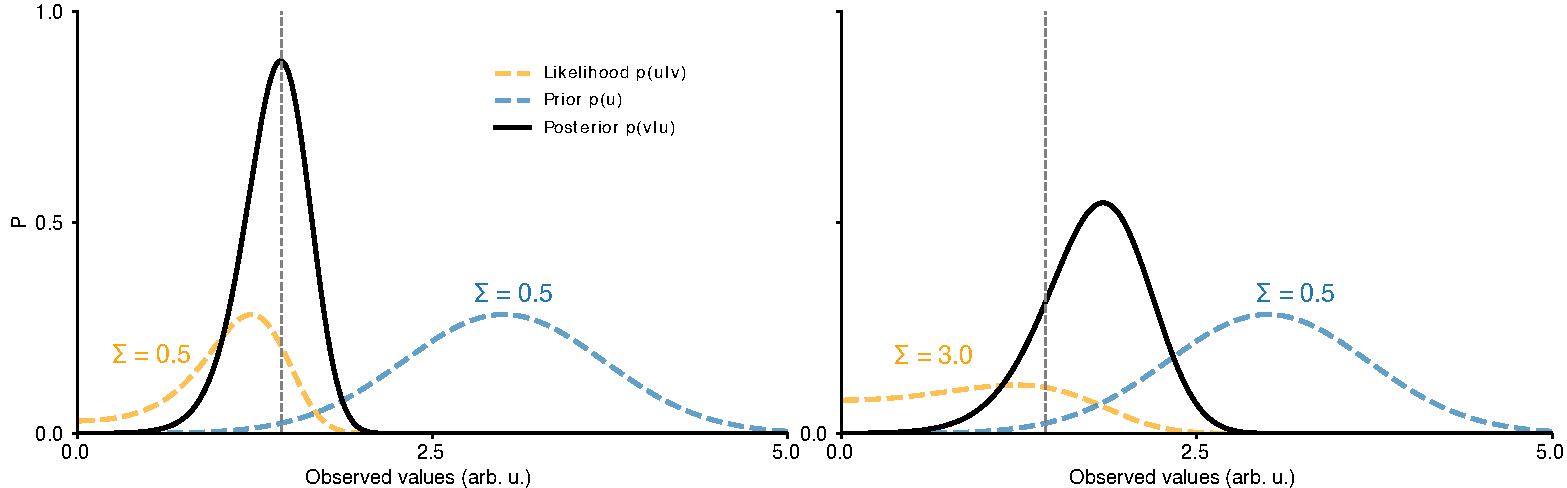
\includegraphics[width=1.\textwidth]{fig/chap2_fig_equi_proba_var.pdf}
\caption[The role of variance in Bayesian integration.]{The role of variance in Bayesian integration. (left) As in Figure \ref{fig_chap2_equi_proba}, Bayesian integration with $\Sigma_u = \Sigma_p = 0.5$. The most likely value of $v$ is indicated by a gray dashed line. (right) Same but with $\Sigma_u = 6\Sigma_p$, driving the posterior away from the sensory likelihood.}
\label{fig_chap2_equi_proba_var}
\end{figure}

This relates to a number of fascinating emergent properties in neural system which will be discussed in later parts of the introduction, namely of neuromodulation~\cite{friston2005theory}, attention~\cite{kanai2015cerebral} and even psychiatric disorders~\cite{adams2013computational, perrinet2014active}. This also speaks of a hierarchy of prediction and prediction errors, whose multiple integration levels are driven by the relative variance of external inputs and internal predictions. Whilst this is discussed more in details in the implementation part of the introduction, we can already state that low-level prediction errors, like the one encoded in \gls{V1}, are tightly bound to the variance of the sensory input, and computationally, learning such variance allows to learn about the extrinsic variability of the external world (see chapter 3). This also allows the visual system to factor in the intrinsic variability of its sensors~\cite{faisal2005ion, faisal2008noise}. 

We shall see in the coming section that the abundance of generic ideas about variance is counterbalanced by the lack of specific neurobiological and neurocomputational literature at the implementational level. As this portion of the introduction is exclusively focused on algorithmic-level concepts, we will not delve deeper into variance at this point. Instead, we will now be focused on computations that can be done on the variance of sensory input, i.e. the likelihood $p(u|v)$.



\newpage 



\section{The two-fold approach to the problem under study}
Having clarified the computational 'why' and algorithmic 'what' of our undertaking, we now turn to the 'how' of its implementation - Marr's final level of analysis, the implementational level, a final stage where our theoretical statements comes to fruition. As previously done, this section aims to provide an overview of the relevant parts of the literature whilst refraining from being a bullet-point detailed list. This is especially the case in the neurobiological section of this introduction, which is concerned with the actual realization of our theories, rather than their experimental aspects, which will be reserved for the introduction of their respective chapters.



\subsection{The in-silico implementational level: Neurocomputations}
The first part of this introduction to the implementational level involves transitioning from the theoretical underpinnings of predictive coding under the free energy principle, towards a practical model that can effectively be employed in vision.



\subsubsection{Predictive coding for vision}
As stated in Equation \ref{eq_df_derror_final}, every single variable required by our formulation of predictive coding can be expressed in terms of a graph with local variables. Such network can be represented as in Figure \ref{fig_chap2_pc_graphs}.

\begin{figure}[h!tbp]
\vspace{0.5cm}
\centering
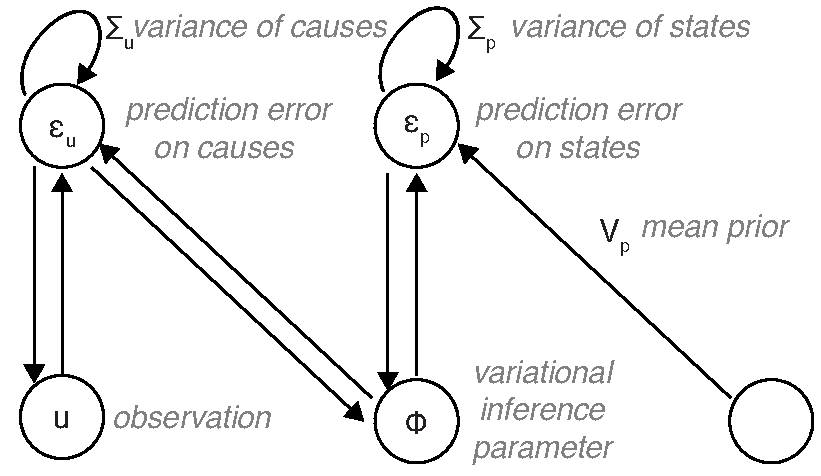
\includegraphics[width=.85\textwidth]{fig/chap2_fig_pc_graph.pdf}
\caption[A simple predictive coding graph.]{A simple predictive coding graph, with helpful reminder of the variables nomenclature in gray.}
\label{fig_chap2_pc_graphs}
\end{figure}

This network constitutes what is known as an acyclic computational graph, a generalized method of articulating problems to topology that will prove useful in chapter~5. Empirical studies have also shown that predictive coding can perform on par (or even better) than the main method of training deep neural networks along such a graph~\cite{millidge2022predictive}, a method known as backpropagation~\cite{lecun1989backpropagation}. This important property helps us scale such a graph beyond the unidimensional form, as we have been doing so far, to a form where "nodes" of the graphs (neurons) would for example represent multiple different orientation in the visual field, as in Figure \ref{fig_chap2_pc_matrix_graphs}.

\begin{figure}[h!tbp]
\vspace{0.5cm}
\centering
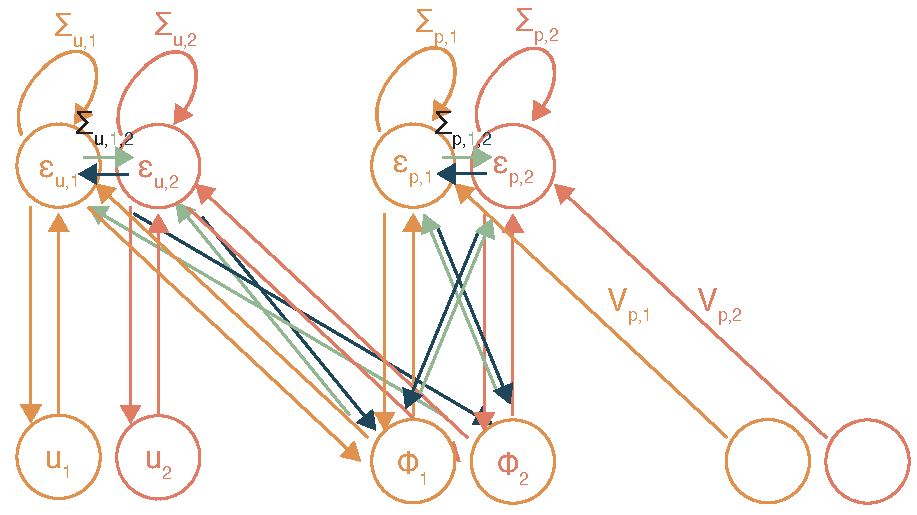
\includegraphics[width=.85\textwidth]{fig/chap2_fig_pc_graph_matrix.pdf}
\caption[A matrix form predictive coding graph.]{A matrix form (with two elements) of the previous predictive coding graph, with additional inter-matrix elements connections colored in green and dark blue.}
\label{fig_chap2_pc_matrix_graphs}
\end{figure}

Following the derivations of Appendix~\ref{appendix_maths}, such network then becomes, in matrix notation, where $\mathit{x}$ is a scalar, $\bar{x}$ a vector and $\mathbf{x}$ a matrix:
\begin{equation}
    \begin{aligned}
       \dot{\bar{\varepsilon}}_p &= \bar{\phi} - \bar{v}_p - \mathbf{\Sigma_p}\bar{\varepsilon}_p \\
       \dot{\bar{\varepsilon}}_u &= \bar{u} - g(\bar{\phi}) - \mathbf{\Sigma_u}\bar{\varepsilon}_u
    \end{aligned}
\end{equation}

with the dynamics of the matrices being:
\begin{equation}
\label{eq_pc_matrix}
    \begin{aligned}
        \frac{\delta F}{\delta \bar{v_p}} &= \bar{\epsilon}_p \\
        \frac{\delta F}{\delta \boldsymbol{\Sigma_p}} &= \frac{1}{2}(\bar{\epsilon}_p\bar{\epsilon}_p^T - \boldsymbol{\Sigma_p^{-1}}) \\
        \frac{\delta F}{\delta \boldsymbol{\Sigma_u}} &= \frac{1}{2}(\bar{\epsilon}_u\bar{\epsilon}_u^T - \boldsymbol{\Sigma_u^{-1}})
    \end{aligned}
\end{equation}

This approach is extremely useful to us, as it allows us to incorporate multiple sensory inputs to the network, like multiple oriented edges to \gls{V1}, which is a critical aspect of the implementational challenge in this thesis. Sadly, it also introduces a major complication, because the inverse variances represented by $\boldsymbol{\Sigma^{-1}}$ now require matrix inversion. This necessitates a network-wide computation, implying that all nodes must access the entirety of the data instantaneously, which is not biologically plausible. Further, such matrix inversion is computationally demanding~\cite{csanky1975fast}, which is one reason why inverse variance weighting is mostly absent from existing predictive coding implementations.
This now presents us with the first implementational issue related to the computations we have detailed so far: trying to incorporate the algorithms we have designed into a formulation that is biologically plausible. While numerous solutions exist~\cite{friston2005theory, bogacz2017tutorial, kanai2015cerebral}, we shall continue one that is naturally suited to matrix forms~\cite{bogacz2017tutorial} and involves the addition of an extra inhibitory neuron, as in Figure \ref{fig_chap2_pc_matrix_graphs_inhibitory}.

\begin{figure}[h!tbp]
\vspace{0.5cm}
\centering
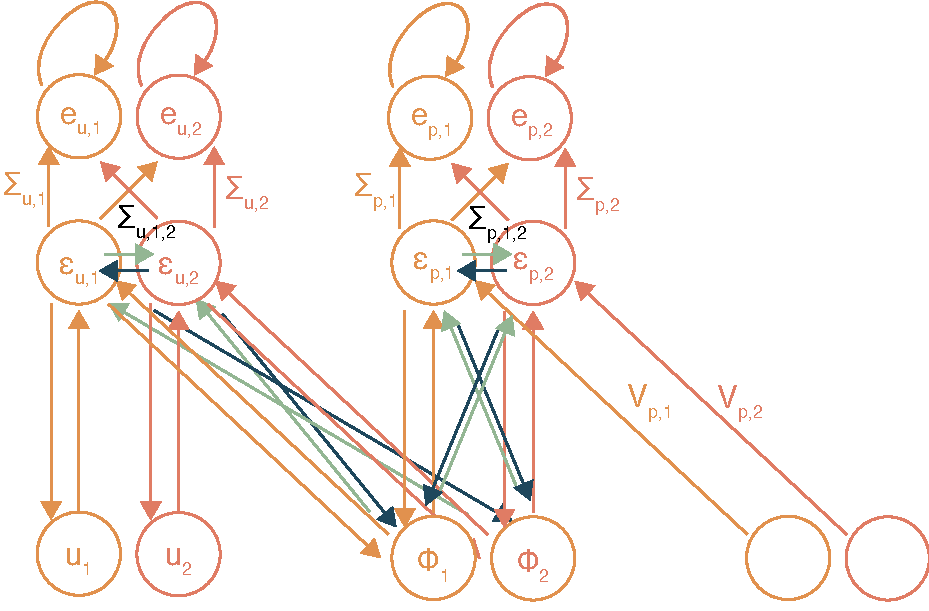
\includegraphics[width=.8\textwidth]{fig/chap2_fig_pc_graph_matrix_hebbian.pdf}
\caption[A matrix form predictive coding graph with Hebbian variables.]{A matrix form predictive coding graph with Hebbian variables.}
\label{fig_chap2_pc_matrix_graphs_inhibitory}
\end{figure}

Based on the notions developed in the final section of Appendix \ref{appendix_maths}, the equation of the prediction errors of the network thus becomes:
\begin{equation}
    \begin{aligned}
\dot{\bar{\varepsilon}}_p &= \bar{\phi}_p - g(\bar{\phi}_{i+1}) - \bar{e}_p  \\
\dot{\bar{e}}_p &= \mathbf{\Sigma_p} \bar{\varepsilon}_p - \bar{e}_p 
    \end{aligned}
\end{equation}
where $e_i$ represents the additional inhibitory neuron. This implementation answers our needs for being able to handle the uncertain nature of vision through learned $\Sigma$ matrices, as detailed in the computational part of the introduction, while also being able to transcribe all the equations of the computational part of the introduction into a tangible and useful form.

But where does the "predictive" aspect of this predictive coding stem from ? This type of modelling can be traced back to \gls{V1} models developed by Rao and Ballard~\cite{rao1999predictive}, who transformed what was originally a signal processing algorithm developed for unidimensional signals~\cite{makhoul1975linear} into arguably one of the most robust theories in neuroscience~\cite{friston2009predictive}. By deriving the principle of efficient coding~\cite{barlow2001redundancy}, they reasoned that neural networks can all be described as predictive networks, like the one formulated above, and can serve as excellent models for \gls{V1}. This proved to be groundbreaking, even predicting the existence of non-classical phenomena~\cite{rao1999predictive} that previously required dedicated models~\cite{skottun1998model}. The remarkable simplicity and beauty of this approach, carried by the free energy principle, is well captured by a quote from Karl Friston~\cite{friston2018does}:
\begin{displayquote}
''Every decade or so, one reads a paper that makes you think “well, that’s quite remarkable”. [Rao and Ballard] showed that a simple architecture was not only consistent with neuroanatomy and physiology but could also account for a range of subtle response properties [...] \\
This was a significant achievement in its own right; however, the really remarkable thing —at least for me— was the following: in simulating their little piece of synthetic cortex, neuronal dynamics and connectivity optimized the same energy or cost function.''
\end{displayquote}

This breakthrough sets the stage for the tremendous success of predictive coding in artificial neural networks. Such predictive network perform on par with deep neural networks, can classify images datasets, predict complex natural images sequences, among many other remarkable feats. Unfortunately, the inclusion of variance is often overlooked in the implementation of such networks. This is not only due to the added complexity it brings to an already intricate network, but also because most of these networks employ point-based estimates rather than comprehensive Bayesian-like distribution learning. Such gap is exactly the aim of this thesis.

One exceptional aspect of predictive coding, though not extensively addressed in this thesis, is the fundamental idea that the brain must predict its inputs and possess a generative model of the world to account for its interpretations. What amplifies the significance of this is the fact that these generative models are self-invertible~\cite{millidge2021predictive}: practically speaking, one can train them, for instance, to classify objects, then simply reverse the flow of information and have them transformed into generative models of images~\cite{millidge2020relaxing}. An example of this reversal can be found at our \href{https://github.com/neuromorphs/BrainDishSiMulator/blob/main/notebooks/Dishbrain_predictive_coding.ipynb}{GitHub repository}, detailing the work we conducted at Telluride workshop to use predictive (generative) coding models in order to issue commands to in-vitro neurons.

In light of this series of generative/discriminative model, predictive coding also suggests a hierarchical series of explanations, which aligns remarkably well with the hierarchical nature of visual processes~\cite{boutin2021sparse, boutin2022pooling}. At the scale of our focus on \gls{V1}, predictive coding is particularly impactful as there have been numerous attempts to align the computations performed within the cortical "microcolumn" circuits, or microcircuits, with those carried out by predictive coding~\cite{bastos2012canonical}. This serves as the starting point for our bridge towards the biological aspect of our networks~\cite{shipp2016neural}, by employing such theories as a lens to delve into the cortex.

\newpage

\subsubsection{Microcircuits as a bridge from the theory to the cortex}
Having now expressed the problem of probabilistic vision in a form that can be mapped onto a graph, the next step is to transpose that graph into a neural network. In the introductory section related to the neurobiology of vision, we discussed some (controversial~\cite{horton2005cortical}) attempts to identify a recurring circuit in the cortex~\cite{douglas1989canonical, douglas2004neuronal}. As a reminder, such "canonical microcircuit" tracks the flow of information through multiple neurons, and was first established through intracellular recording in the cat's \gls{V1}~\cite{douglas1989canonical} to measure pre- and post-synaptic connectivity and functional strength. According to these studies and others~\cite{thomson2002synaptic}, a feedforward flow of excitatory activity in the cortical microcolumn arises from thalamic inputs to layer IV, then to layer II/III, and finally back to layer V/VI. There is proof that other excitatory pathways that would close the loop only form a minority of connections, namely the layer II/III to layer IV or layer V to layer II/III~\cite{thomson2002synaptic}. Inhibitory pathways in cortical microcolumn are historically harder to make out, namely because such neurons have much more functional subtypes~\cite{gouwens2019classification}, but recent evidences are showing that they can participate in the regulation of the circuit in a layer-specific fashion~\cite{bugeon2022transcriptomic}. Extrinsically, this circuit needs also to be integrated into an input/output scheme compatible with the idea of hierarchical predictive coding~\cite{boutin2022pooling}. Inhibitory connections play here an important role, because they allow multiple such microcircuit to compete against one another at the level of a cortical area~\cite{coultrip1992cortical, chavane2022revisiting} (see also chapter 4). At the macroscale level, backed by anatomical evidence~\cite{markov2014anatomy}, the final concept of a canonical microcircuit is that layer II/III sends synapses to higher order cortical areas~\cite{felleman1991distributed}, as opposed to layer V/VI that sends synapses to lower levels~\cite{markov2011weight}. Based on these considerations, Bastos et al.~\cite{bastos2012canonical} proposed a mapping of our computational graph onto a neural network:

\begin{figure}[h!tbp]
\vspace{0.1cm}
\centering
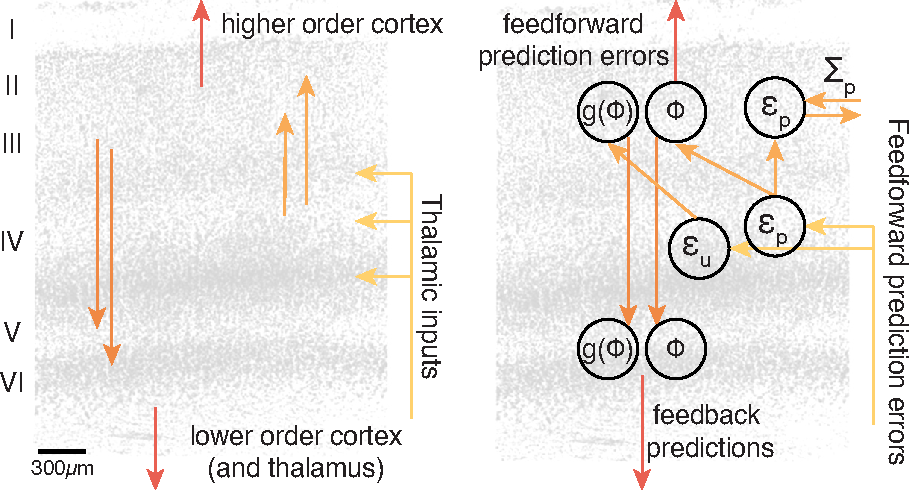
\includegraphics[width=1.\textwidth]{fig/chap2_fig_microcircuit.pdf}
\caption[Canonical microcircuit for predictive coding.]{Canonical microcircuit for predictive coding, with (left) Figure \ref{fig_chap2_vision_V1} for comparison and (right) graph adapted from Bastos~\cite{bastos2012canonical}.}
\label{fig_chap2_microcircuit}
\end{figure}

It now remains to review experimental proofs to back the existence of such predictive circuitry. In that sense, proofs of a canonical microcircuit are somewhat sparse, but there is growing consensus that a canonical microcircuit performing predictive operations does indeed account for experimental results. In this context, the study in chapter 4 provides further experimental support, by validating the idea of mapping input variance to supragranular layers, largely due to their extensive lateral connectivity~\cite{angelucci2002circuits,chavane2022revisiting, adesnik2010lateral}. There is also vast account of the fact that specific types of neurons in microcircuits - namely disinhibitory motifs~\cite{kuhlman2013disinhibitory, naka2016inhibitory} - are performing layer-specific computations~\cite{bugeon2022transcriptomic} that can support learning on-par with predictive coding algorithms~\cite{sacramento2018dendritic}.
Finally, there is also theoretical evidence that show that combining simple elements of neural origin can actually yield neural networks that compute prediction errors in an unsupervised manner~\cite{boerlin2013predictive, hertag2022prediction}.

Further, this model implies that predictions and prediction errors, operating mostly on two separate firing regimes, are reflected in the oscillatory domain (an experimental concept further explored in chapter 7). Based on that observation, there is a mounting evidence that suggest two bands of oscillations for superficial and deep layers of the cortex~\cite{bastos2015visual}. Such oscillatory evidences are numerous~\cite{nikolic2013gamma, schmiedt2014beta, engel2001dynamic, engel2010beta} to show that deep layers oscillate at a low frequency~\cite{bastos2020layer} (which is gated through the pulvinar~\cite{cortes2021corticothalamic}, as contributed in chapter 7) to prepare predictions and make way for the fast oscillations of sensory inputs in upper layers.

On a broader scale, numerous empirical evidences of predictive coding mechanisms at work in the brain have been accumulated, even prior to Friston's initial paper, which we will now explore to further support our approach.



\newpage 



\subsection{The in-vivo implementational level: Neurobiology}
The final part of this introduction to the implementational level involves transitioning from the notion that predictive coding can be used as a framework for this thesis, towards showing proof that there exists both predictive and variance-based computations in the brain.




\subsubsection{Neural evidences of predictive coding}
Having gathered the (sparse) supporting biological evidence for a canonical microcircuit, and having mapped this predictive microcircuit to certain functional activity at the circuit level, we now turn our attention towards assessing whether the brain indeed utilizes predictive coding at a global scale. A bias naturally stems here~\cite{shipp2016neural}, as we will try to explain many disparate phenomena with a single theory - when one perceives every problem as a nail, it becomes convenient to envision a normative theory based on a hammer~\cite{maslow1966psychology}. 

Essentially, as we expressed in Equation \ref{eq_df_derror_final}, predictive coding proposes that the brain increases computational efficiency by transmitting only prediction errors~\cite{friston2005theory}. As such, if a certain visual input does not generate a prediction error, it should not be transmitted, and thus the neural response for predicted stimuli should be weaker than for unpredicted stimuli. Therefore, the first argument that supports the existence of predictive coding in the brain is the experimental observation that repetition of stimuli elicit a diminution of the evoked neural activity. This is observable not just with the visual responses~\cite{summerfield2008neural, summerfield2011human}, but also in the auditory~\cite{garrido2007evoked, todorovic2011prior} and somatosensory cortices. 
Conversely, unexpected or surprising events should trigger an increase in said neural activity. This assertion is also verified within the visual pathways~\cite{pak2021impaired} where the violation of a repetitive pattern induces a significant surge in the firing rate. This effect is also noticeable at the psychophysical level, a neural event known mismatch negativity potential~\cite{alho1995cerebral, wacongne2012neuronal}, which is an entire sub-field on its own (see chapter 7). Further evidences can be found when violating the distribution of natural images~\cite{bair2003time,fiser2004small} (as described in the first section of the introduction), or under many conditions of predictability violation~\cite{kok2012attention, meyer2011statistical,murray2002shape}.

It's also worth noting that the large-scale hierarchical organization of the cortex, particularly the visual cortex~\cite{felleman1991distributed}, aligns well with the principles of predictive coding (Figure~\ref{fig_chap2_brainlevel_pc}). In this representation, the hierarchical organization of the brain emerges from the Bayesian inference process we developed earlier, which relies on a hierarchical conditional model~\cite{friston2006free}. This corresponds well with the layer-specific responses of the microcircuit and their respective feedforward versus feedback connections~\cite{markov2014anatomy}. On a larger scale, this constitutes a recurrent circuit that generalizes the formulation we introduced in Equation~\ref{eq_pc_matrix}: a stable functional model that seeks to minimize prediction errors while continuously updating a prediction-based model of the world.

\begin{figure}[h!tbp]
\vspace{0.5cm}
\centering
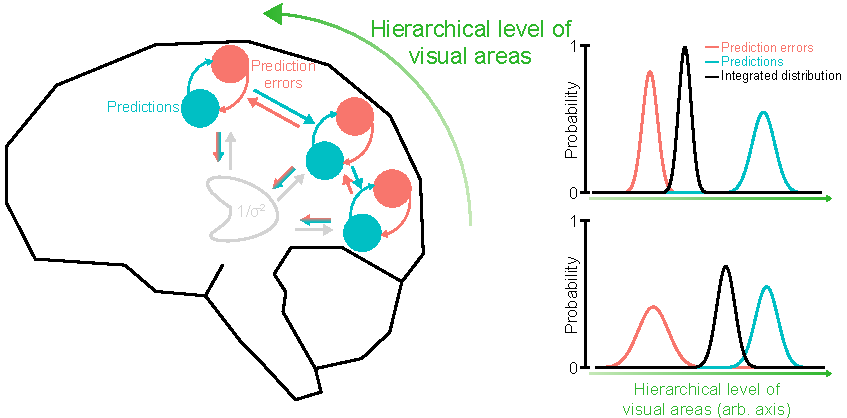
\includegraphics[width=1.\textwidth]{fig/chap2_fig_hierarchical_pc.pdf}
\caption[Hierarchical predictive coding in the brain]{Hierarchical predictive coding in the brain, (left) implemented as a globally and locally recurrent series of prediction errors and prediction integrations. (right) As in Figure \ref{fig_chap2_equi_proba_var}, the effect of the input variance on the predictive model.}
\label{fig_chap2_brainlevel_pc}
\end{figure}

Still on the anatomical side of the argument, the lateral connectivity intra~\gls{V1} merits further mention~\cite{thomson2003interlaminar,chavane2011lateral,katzel2011columnar}, as it provides the support for local competition of orientation-based predictions on the worldly states. This is usually characterized as an attentional mechanism~\cite{friston2012predictive,ainley2016bodily}, but we would contribute here that it takes effect far too rapidly~\cite{ladret2023cortical} for that to be the case. In this thesis, we interpret it as a local mechanism, as formulated by Friston in its original implementation of predictive coding~\cite{friston2005theory}.
Another implementation we will discuss in chapter 7 involves a globally parallelized (through the pulvinar) implementation of variance~\cite{kanai2015cerebral}, that allows the brain to determine which visual areas best explain the current environment. This is experimentally corroborated by the fact that pulvinar modulations essentially constitute contextual modulations~\cite{robinson1992pulvinar, casanova2001higher,de2020pulvinar} dynamically applying context to the content processed by the cortex~\cite{purushothaman2012gating}.

In addition to these findings, predictive coding has been shown to effectively model pathological conditions of the brain, an emerging field referred to as computational psychiatry~\cite{adams2013computational}.  While it's too premature to label this as evidence, the wide adoption~\cite{grenander1998computational} of this framework is a compelling argument supporting the idea of the brain functioning as a predictive system. In that framework, the idea that shifts in variance can move one closer or further from the prior, as demonstrated in Figure~\ref{fig_chap2_brainlevel_pc} (and in the Conclusion of this manuscript), provides a fitting description of disorders characterized by hypo-variant priors (such as autism~\cite{van2013predictive, van2014precise}) or hyper-variant priors (like schizophrenia~\cite{horga2014deficits}). This now paves the way for the end of this (lengthy) introduction, with a final (and not lengthy) section dedicated to the representation of variance in the predictive brain.

\newpage

\subsubsection{Neural representations of variance}
Having mapped predictive models onto some biological substrates, it is now time to explore whether there is empirical biological evidence supporting the representation of variance. Unfortunately, this field of investigation is not an expansive one, as reflected by the length of this section. What sparse evidence exist is however very promising, and in line with our respective contributions in chapters 3 to 8.

The seminal work in this field is a study by Orban et al.~\cite{orban2016neural}, which shows that local computations performed between orientation detectors can effectively process orientation variance, as that competition, through inhibition, increases the spike-to-spike variance of the neural activity. Thus, elegantly, the variance of an internal representation can be "signaled" by the variance of the activity supporting it. This aligns well with the psychophysical literature we introduced earlier~\cite{heeley1989width}, specifically the notion that competition among orientation detectors accounts for the psychophysical observations of human subjects. 

On the biological front, if we refrain from considering the superposition of two gratings as a distribution of orientation, as was historically done~\cite{geisler2001motion} (although some approximation hold~\cite{furmanski2000oblique,li2003oblique}), the whole idea of encoding orientation variance in \gls{V1} was actually pioneered by Goris et al.~\cite{goris2015origin}. They reported that heterogeneously tuned \gls{V1} populations help encode the orientation distributions found in natural images, and that this functional diversity could be accounted for by a linear-nonlinear (L-NL) model. While this could explain the diversity of tuning in the data we report in chapter 4, we will find that in terms of modeling, competition among orientation detectors within a predictive context remains the best descriptor~\cite{ladret2023cortical}. 

\begin{figure}[h!tbp]
\vspace{0.1cm}
\centering
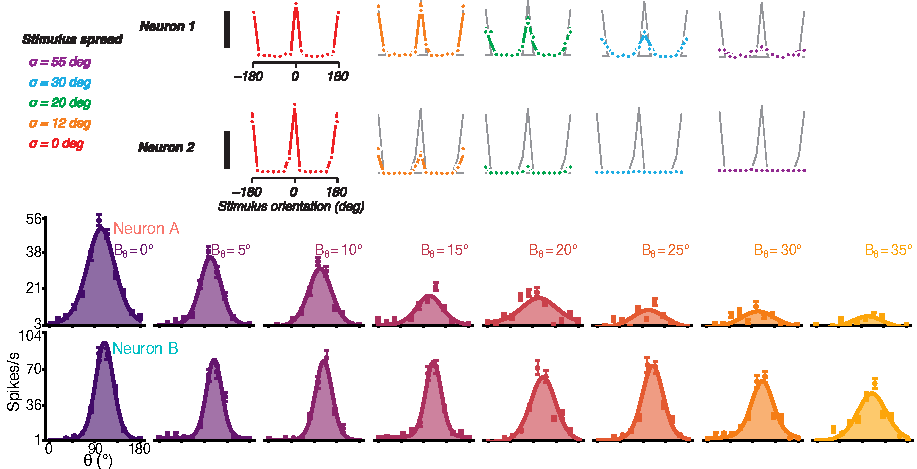
\includegraphics[width=1.\textwidth]{fig/chap2_fig_goris.pdf}
\caption[Active modulation of neurons by orientation variance.]{Modulation of tuning curves by orientation variance. (Top) Goris et al.~\cite{goris2015origin}. (Bottom) This thesis~\cite{ladret2023cortical}.}
\label{fig_chap2_neuralvariance}
\end{figure}

Considering the sparse nature of the relevant literature, referencing our own work from chapter 4 here feels necessary. Our study reaffirms the findings in the literature on anesthetized macaques~\cite{goris2015origin}, as we identified single-neuron variance modulations that underpin the decoding of orientation variance at the population level in \gls{V1}. This suggests that a shared neural mechanism may exist in both felines and primates, which isn't surprising given the crucial role of variance for the proper encoding of natural images in \gls{V1}~\cite{olshausen1996emergence}, a point we've emphasized repeatedly throughout this introduction. 

Our specific contribution here is connecting these findings to cortical layers, strengthening the idea that supragranular neurons with sharp tuning and slow dynamics~\cite{ringach1997dynamics,ringach2002orientation} facilitate the concurrent encoding of orientation and its variance. This links nicely with the concept of cortical microcircuit introduced earlier, as ten years prior to our article, it was proposed that supragranular activity should encode variance, a hypothesis for which we have provided formal experimental evidence in this thesis.

As far as biological evidences are concerned, there is consensus across studies that heterogeneity and local competition, i.e., intra-V1 activity, are sufficient to explain all observations. In fact, both neurobiological and computational evidence suggest that \gls{V1} doesn't need to enlist other cortical areas to process orientation variance, but that such process in other cortical areas might actually be part of synchronized global computations (more in chapter 7). 

For instance, the heterogeneous recurrent excitatory and inhibitory synaptic connectivity in \gls{V1}~\cite{jia2010dendritic, chen2011functional, iacaruso2017synaptic, scholl2017local} sustains resilient orientation tuning~\cite{monier2003orientation} that can account for the diversity of single neurons' resilience under different connectivity profiles, as explored in our computational model~\cite{ladret2023cortical}.
This is supported by the temporal scale of local recurrent connectivity, namely the slowly-conducted horizontal waves in an orientation map~\cite{chavane2011lateral}, which fits the view of variance processing as an iterative and accumulative computation implemented by local recurrent interactions between supragranular resilient neurons that are heavily connected through recurrent interactions with neighboring cortical columns~\cite{douglas1989canonical,ringach1997dynamics,ringach2002orientation, chavane2011lateral}. 

Despite the limited quantity of available evidence, the existing findings notably converge. Whether across species, research teams or functional encoding schemes, the overarching theme remains constant: there is an active encoding of variance in the primary visual cortex. Having established this, we can now proceed to explore the main section, beginning with the exploration of the structure of variance in natural images, which will then directly link to the findings in chapter 4.

	\chapter{Variance in Vision Models: a Convolutional Sparse Coding Approach}

\begin{flushright}
    \textit{''These stats are staggering \\
    Had his Ph.D in indiscreet street haggling.''} \\
    MF Doom, Gazzillion Ear, 2009

    %\textit{''The proof of the pudding is in the eating.''}\\
    %British proverb
\end{flushright}

%\begin{flushright}
%    \textit{''As far as the laws of mathematics refer to reality, they are not certain;\\
%    and as far as they are certain, they do not refer to reality.''}\\
%    Albert Einstein, Lecture at the Prussian Academy of Science in Berlin, 1921
%\end{flushright}

\chaptertoc{}

\section{Introduction: Orientation, Statistics, and Orientation Statistics}
As introduced in the previous chapter, a central role of the brain is to build a model of its environment in order to enact complex behaviors. One key component of these models is their reliance on internal representations of the environment. While this is true in predictive coding (where these representations are predictions), it also forms the dominant narrative in neuroscience~\cite{keller2018predictive}. This understanding of the brain stems from the discovery of the receptive field, by Sherrigton's seminal studies~\cite{sherrington1906observations}, which correlated a neural discharge pattern with an element of the environment (here, stroking a certain skin spot). Iteration upon iteration of related research have built modern neuroscience upon a similar narrative, starting with the "fly detectors" neurons of Barlow~\cite{barlow1956retinal}, the orientation selective neurons of Hubel and Wiesel~\cite{hubel1959receptive}, the place cells of O'Keefe and Dostrovsky~\cite{o1971hippocampus}, the grid cells of Hafting~\cite{hafting2005microstructure}, the face cells of Perret~\cite{perrett1982visual}, and so on~\cite{martin1994brief}. 

In vision, there is thus no denying that orientation forms the basis of these models of the world internalized in the brain. One legitimate question that should be asked before diving into $4$ chapters of studies related to orientation selectivity could be: "why orientations in the first place" ? As history would have it, Hubel and Wiesel discovery was somewhat serendipitous~\cite{martin1994brief}, and orientation selectivity was discovered somewhat accidentally when the two scientists noticed strong neural responses as they were inserting a glass slide (used to project the spots of light) into the projector of their cat experiments. It thus become evident that neurons in \gls{V1} were in fact responding not to spots of light, as in the retina and \gls{LGN}, but to the edge of the glass slide, indicating a selectivity for oriented edges. 

Had computational neuroscience been $30$ years more advanced at the time of these experiments, Hubel and Wiesel might have had the chance of knowing what to look for in the first place, rather than stumble upon it semi-accidentally. Indeed, we have said that a key property of the brain is efficient coding~\cite{barlow1961possible}, which saves costly neurobiological message passing by encoding solely relevant information. Under predictive coding, for example, this means solely transmitting prediction errors. This generic principle imposes a constraint of sparseness on the message to be sent by neurons, meaning using as little energy as possible while maintaining a highly accurate internal model. Thus, one can envision early sensory cortices as models of the world build through the transformation of dense redundant inputs into sparse efficient representations. By creating a computer model that performs high-quality reconstruction with as little activity as possible, one can thus see what types of features are ideal to deconstruct any given type of sensory input. This trade-off has been explored by Olshausen and Field~\cite{olshausen1996emergence}, who showed that a model of natural images with a constraint of sparsity yields receptive fields that are extremely similar to those found in \gls{V1} (Figure~\ref{fig_chap3_olshausen}). Thus, a low-level invariant representation of the (static) visual world can be created using edges detector.

\begin{figure}[h!tbp]
\vspace{0.1cm}
\centering
\includegraphics[width=1.\textwidth]{fig/chap3_olshausen.pdf}
\caption[Natural images and sparse dictionaries.]{Natural images and sparse dictionaries. 
(left) Natural images components, extracted using Principal Component Analysis (PCA). 
(middle) Dictionaries yielded by learning a sparse code on natural images, from~\cite{olshausen1996emergence}. 
(right) Comparison with macaque \gls{V1} receptive fields, from~\cite{ringach2002orientation}.}
\label{fig_chap3_olshausen}
\end{figure}

The statistical distribution of these edges in any given image follows a characteristic pattern~\cite{perrinet2015edge}, and given optimal modelling, these statistics are the main constraint upon which further sensory processing relies~\cite{olshausen1997sparse}. Most of these oriented edges are represented at the cardinals points, that is, horizontally and vertically~\cite{coppola1998distribution}. This is echoed at the neuronal level by a cardinal bias in visual perception~\cite{hansen2004horizontal}. As we will show in this chapter's article, around either of these main orientations, the distribution of oriented elements can be characterized by its first- and second-order moments: a median orientation, and its corresponding (inverse) variance. A proper model of a natural images thus depends on a proper model of both these moments (Figure~\ref{fig_chap3_ori_distrib}), which is reflected in the response properties of primary visual cortex neurons that have diverse orientation and variance~\cite{hubel1962receptive}. 

\begin{figure}[h!tbp]
\vspace{0.1cm}
\centering
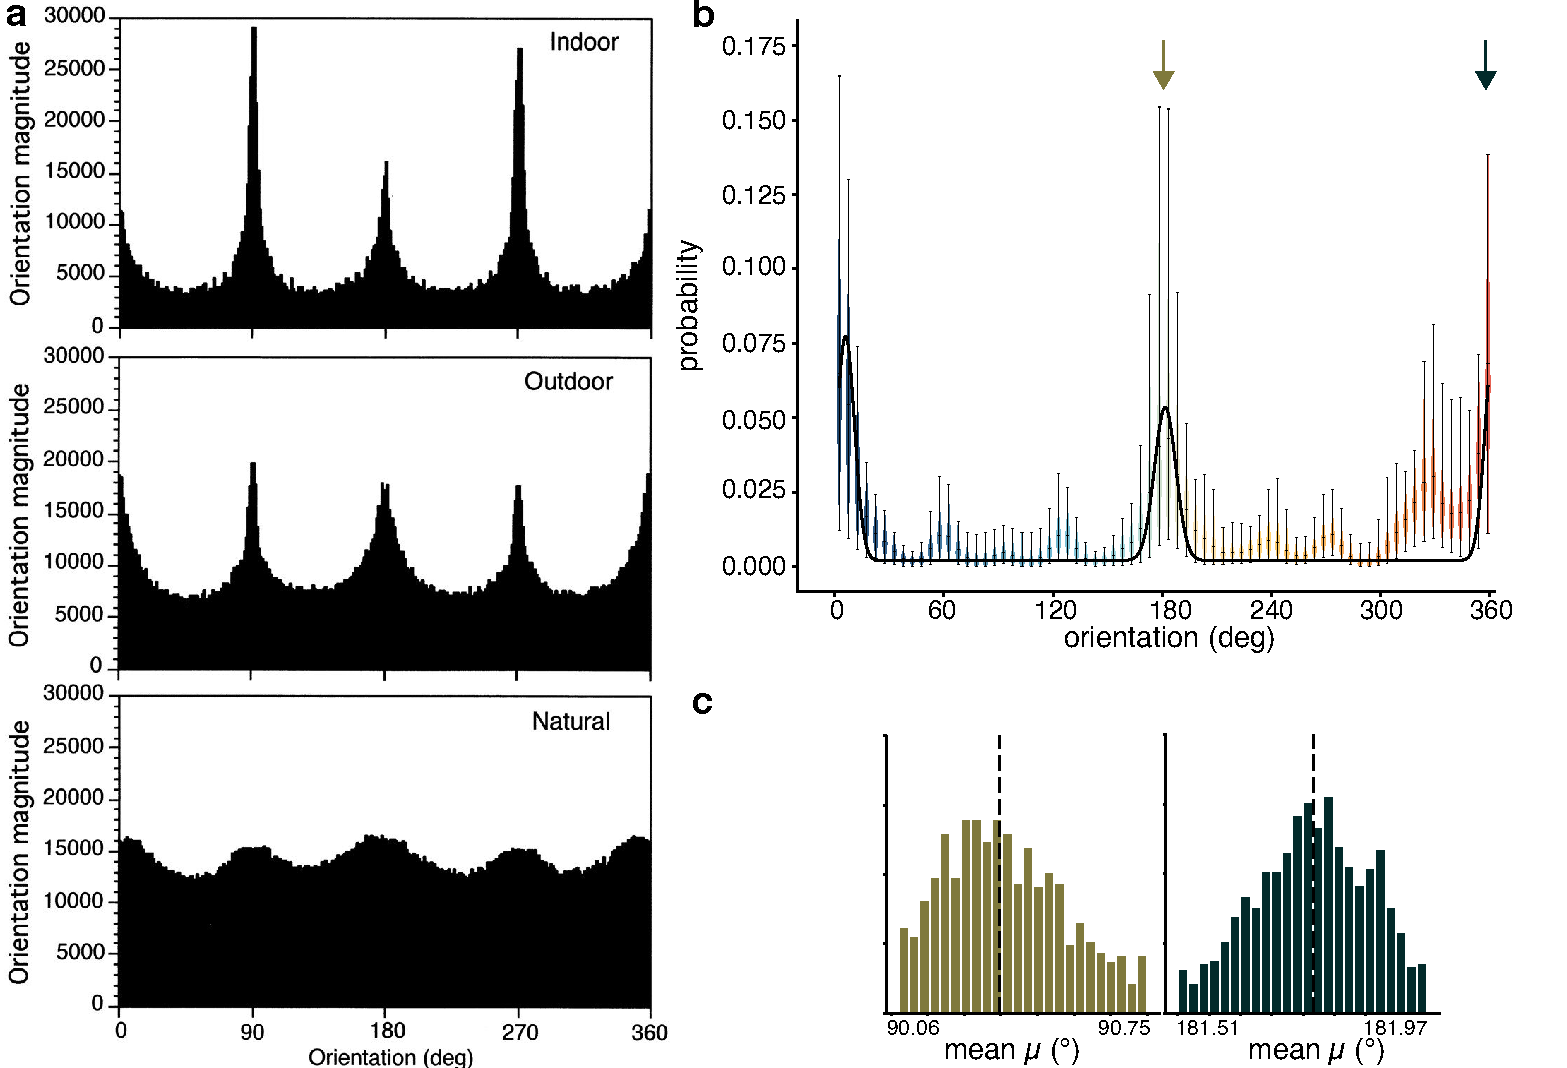
\includegraphics[width=1.\textwidth]{fig/chap3_ori_distrib.pdf}
\caption[Distribution of orientations in natural images.]{Distribution of orientations in natural images.
(a) Distribution of oriented contours, extracted by Sobel filters (see this chapter's article), as done in~\cite{coppola1998distribution}. 
(b) Distribution of oriented contours, extracted by Sparse Coding (as done in this chapter's article), with mean von Mises distribution in black. 
(c) Distribution of means of two peaks of the distributions, for each image.}
\label{fig_chap3_ori_distrib}
\end{figure}

If orientations in natural images follow such a prototypical distribution, then what is the optimal neural code to represent them ? This question is one of uncertainties. Uncertainty on how the image's orientation deviates from the typical distribution is a problem of uncertainty bound to the input, called aleatoric uncertainty. Uncertainty on how to best model these images is a problem of uncertainty bound to the model, referred to as epistemic uncertainty. Aleatoric uncertainty is linked to the variance of the distribution of orientation: the higher the variance, the more spread the input is (in orientation space), and thus the less certain the information is. As stated in the introduction, linking this aleatoric uncertainty/variance to the uncertainty of the model is crucial for Bayesian processing, which provides explicit rules to do so (see Equation~\ref{eq_proba_intro}). 

This chapter serves to characterize natural images as Gaussian (or here, von-Mises) distributions of oriented features, which allows us to keep working within the mathematical framework described in the introduction. This further serves as a justification of Gaussian distribution of orientation as stimuli for animal recordings in chapter 4. Second, it serves to understand how the variance of natural images can be processed by a model with no explicit learning rules for variance. This, again, is useful to describe variance interactions as an emergent property throughout this thesis. Third, as we'll delve into in this chapter's conclusion, this perspective enables us to examine the trade-off between two encoding strategies. One approach involves dense sampling using numerous neurons, providing high quality reconstruction but at a higher energy cost. The alternative employs sparse sampling, where fewer neurons co-encode features and their variance. Under the right conditions, this latter strategy can be equally performant, but much more energy-efficient.

\section{Methods: Sparse Coding}
\begin{figure}[h!tbp]
\vspace{0.1cm}
\centering
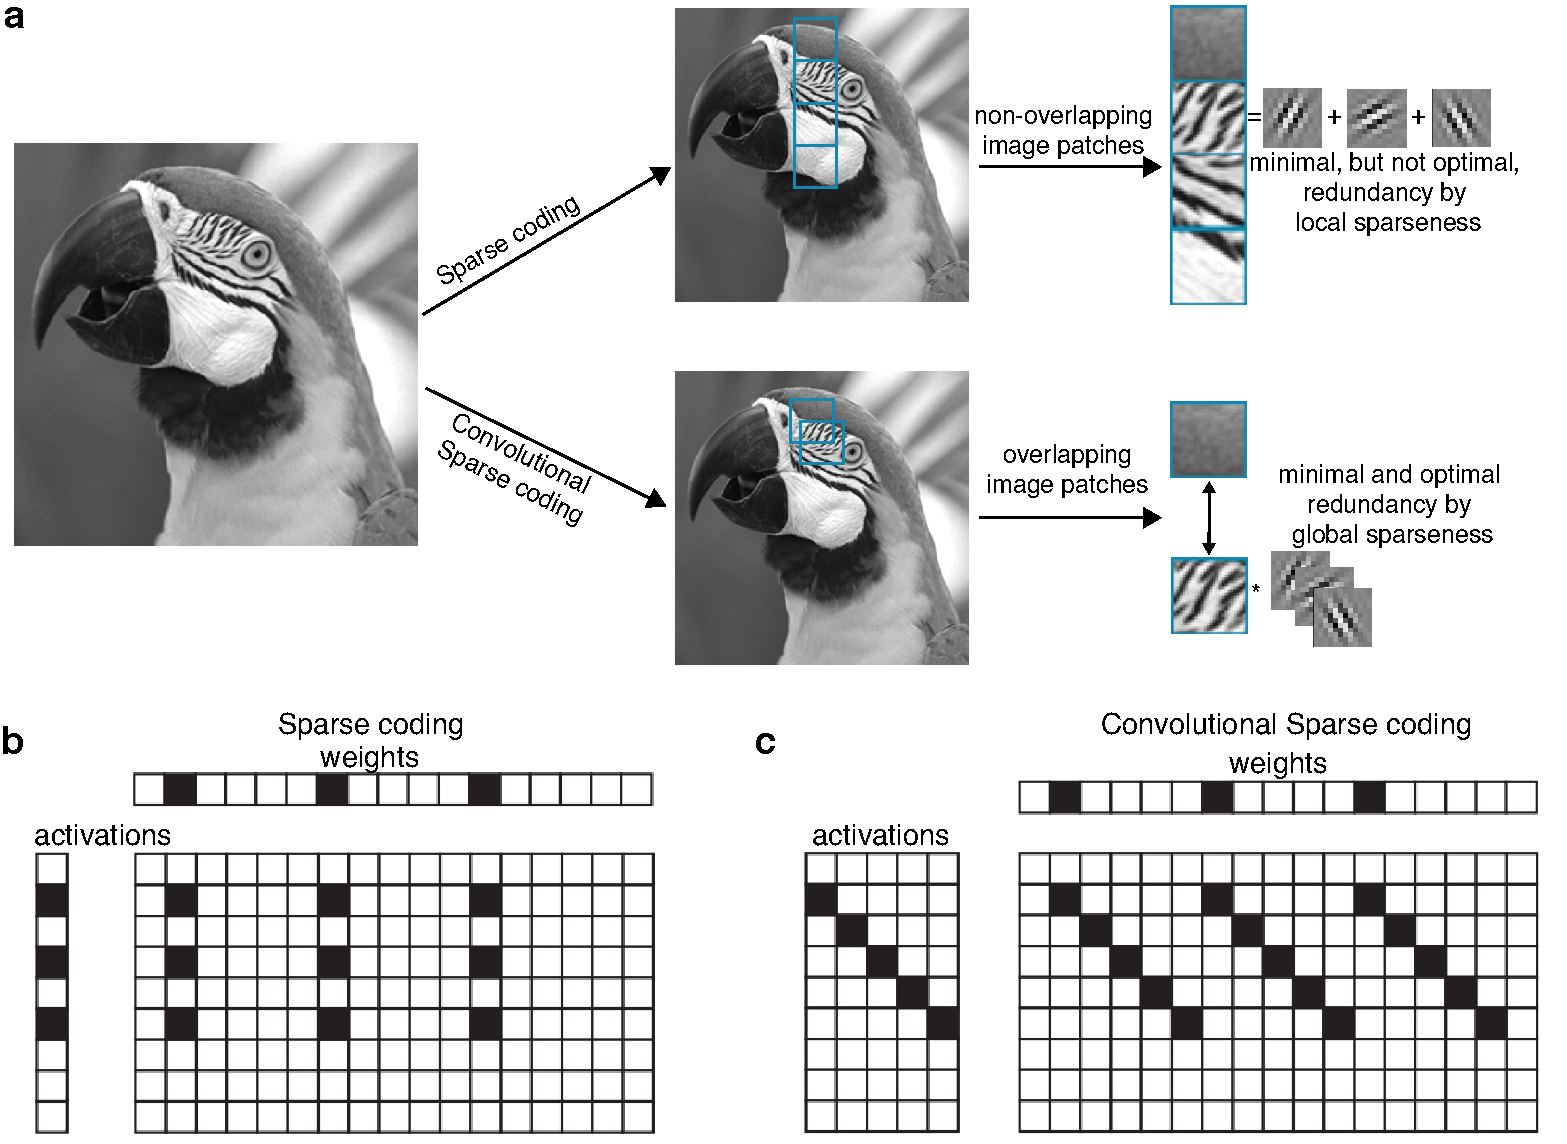
\includegraphics[width=1.\textwidth]{fig/chap3_csc.pdf}
\caption[Convolutional Sparse Coding.]{(a) Convolutional Sparse Coding (bottom) relies on convolution operations to achieve global sparseness and remove local redundancies (top), mimicking the operation of the visual system. (b) and (c), visualized as vector-vector or vector-matrix products.}
\label{fig_chap3_csc}
\end{figure}

The model used by Olshausen and Field~\cite{olshausen1996emergence} to show the emergence of orientation selectivity in sparsely-constrained algorithm is referred to as Sparse Coding (SC), and is a widely used model for learning the inverse representation of an input signal. Given the assumption that a signal can be represented as a linear mixture of basis functions (in neurobiological terms, receptive fields), the optimization problem solved by sparse coding is one that tries to minimize the number of basis functions that are used to represent the input signal (which would be spikes), yielding a compact and efficient representation of the original signal. Here, we framed sparse coding as the problem of reconstructing an image $s$ from sparse representations $x$ while minimizing a $\text{L}_1$ norm of the representation. This problem can be approached with a Basis Pursuit DeNoising (BPDN) algorithm:
\begin{equation} 
    \underset{x}{\operatorname{arg min}} \frac{1}{2} || s - D x ||^2_2 + \lambda ||x ||_1
\end{equation} 
where $D$ is a dictionary (i.e. a set of basis functions used to represent $s$) and $\lambda$ a regularization parameter that controls the trade-off between fidelity and sparsity. The present article uses a variation of sparse coding, Convolutional Sparse Coding (CSC), which, as the name implies, relies on the convolution operator: 
\begin{equation} \label{eq:csc}
    \underset{\{x_k\}}{\operatorname{arg min}} \frac{1}{2}
    || s - \sum_{k=1}^K \text{d}_k \ast x_k ||^2_2 + 
    \lambda \sum_{k=1}^K ||x_k||_1
\end{equation}
where $x_k$ is an $N^2$ dimensional coefficient map (given an $N^2$ sized image), $\text{d}_k$ is one kernel (among $K$ channels) and $\ast$ is the convolution operator (Figure~\ref{fig_chap3_csc}). One additional advantage of convolutional sparse coding over other reconstruction techniques is its ability to learn interpretable features from the data, which can be easily visualized and understood by human experimenters~\cite{boutin2020sparse}. 

\section{Methods: Deep Learning}
The final section of this article uses a Deep Neural Network, as a model to understand how the sparse code can be of use in further stage of visual hierarchical processing. While they are not used elsewhere in this thesis, a brief introduction can be useful. All modern artificial neural networks rely on the gradient descent algorithm, as introduced by Rumelhart~\cite{rumelhart1986learning}. The essence of this optimizer is to iteratively adjust the parameters of a neural network to minimize a loss function, defined as the difference between its predictions and the actual data.

Given this loss function \(L(\theta)\), where \(\theta\) represents the parameters of the network, the gradient descent update rule is expressed as:
\begin{equation}
\theta_{t+1} = \theta_t - \alpha \nabla L(\theta_t)
\end{equation}
where \(\theta_{t+1}\) is the updated parameter at iteration \(t+1\), \(\alpha\) is the learning rate, and \(\nabla L(\theta_t)\) is the gradient of the loss with respect to the parameters at iteration \(t\).

Here, we use a Convolutional Neural Network, as introduced by LeCun et al.~\cite{lecun1998gradient} to demonstrate the capability of learning hierarchical features is a central model in Deep Learning for processing grid-like topology data, such as images. This model is based on the idea that an input signal can be represented through a hierarchical set of layers, where each layer transforms the input data with the aim of gradually abstracting the features of the data to enable effective classification or regression at the output layer.

Given an input image \(I\), a Convolutional Neural Network seeks to learn a hierarchy of convolutional features \(F\) by applying a series of convolutional and pooling operations, typically defined as:
\begin{equation}
F_l = \operatorname{ReLU}(W_l \ast F_{l-1} + b_l)
\end{equation}
where \(F_l\) is the feature map at layer \(l\), \(W_l\) is the convolutional kernel, \(b_l\) is the bias term, and \(\ast\) is the convolution operator.

Deeper architectures, that is, with more layers, also contain a MaxPooling operation which groups representations into an intermediate, dense form: 
\begin{equation}
F_{\text{deep}} = \operatorname{MaxPooling}(\operatorname{ReLU}(W_{\text{deep}} \ast F_{\text{prev}} + b_{\text{deep}}))
\end{equation}
where \(F_{\text{deep}}\) represents the deeply learned features, and \(F_{\text{prev}}\) is the feature map from the previous layer. These Deep Convolutional Neural Networks, with their deep architectures, have an advantage over other models due to their capability to learn more abstract and generalized representations of input data, which are critical for solving complex problems in computer vision~\cite{krizhevsky2012imagenet}. In this study, we leverage this capability to understand how the representation power of deep layers influences the performance of the model. Each DCNNs has its particular architectural tweaks, for which we would refer the reader to the article in the next section.

\section{Article: "Sparse Representation of Natural Images with Heterogeneous Orientation Kernels"}
The following article is the initial contribution of this thesis, framing natural images as Gaussian-like distribution of oriented elements. This alleviates major non-linear integration difficulties that would otherwise be present in the predictive coding framework, and serves as a justification of the use of Motion Clouds~\cite{leon2012motion} in the next chapter. On its own, the article uses dictionaries of receptive fields that emphasize two coding strategies to reconstruct natural images: focusing either on median features (orientations) or their variance (bandwidths). We show that focusing on the former improves reconstruction, while the latter improves sparseness. Fine-tuning through learning on a dataset of natural images alleviates this compromise, allowing optimal encoding of natural images through a sparse co-encoding strategy, as will be also uncovered in \gls{V1} in chapter 4.  

Full citation is as follows: \fullcite{ladret2023kernel}
% avant d'intégrer un article dans votre thèse, consulter http://www.sherpa.ac.uk/romeo/ si vous souhaitez diffuser sur internet
\includepdfset{pagecommand=\thispagestyle{scrheadings}} % ajoute la numérotation continue des pages aux fichiers pdf importés
\includepdf[scale=1.0,pages=-]{papers/neuralcomp.pdf} % 'scale' ajuste la taille du pdf, vous pouvez affiner en fonction des marges

\section{Conclusion}
Designing an efficient strategy to represent our environment is challenging, especially in a world loaded with statistical variance. Modelling such modelling visual inputs with unpredictable variance is the focal point of this thesis. In the current article, we developed a computational model that learns an optimal representation of natural images, and explored the sparseness/reconstruction trade-off of its receptive fields. By using sparse coding as a way to extract the features necessary to build a representation of natural images, we showed that a neural representation of variance is advantageous, even at the level of Deep Learning research. This ties directly to Bayesian processing, which explicitly derive mathematical rules that integrate both epistemic and aleatoric variances are advantageous (see Equation~\ref{eq_proba_intro}). In contrast, our study concentrates on an implicit emergent encoding of the epistemic and aleatoric variances. This also relates to the idea that computation of variance can be seen as an emergent property, which will be further emphasized in the next chapter. 

A research offspring that will directly stem from this work is to train Deep Neural Networks directly on sparse coefficients that encode an optimal representation of images, rather than images themselves. The preliminary practical work on that end has already been made here, as our codebase in the article consisted of porting a sparse coding library (SPORCO~\cite{wohlberg2017sporco}) into a tensor format~\cite{paszke2017automatic}, allowing for milliseconds-fast computations. Sparse representations, whether here or in the brain, are essentially distributions of binary events weighted by synaptic connectivity. As these Deep Neural Networks relying on spiking activity are set to eventually surpass regular methods~\cite{eshraghian2022memristor, grimaldi2023learning}, there would be great advantage in integrating the work done here in a spiking framework. One final advantageous effect of these sparse representations is their natural property to remove noise in the input. Thus, an encoder that transforms natural images into sparse representations with variance could easily defend against noisy inputs (whether malicious or not), which would prove useful in critical applications such as medical imaging. 

Aside from these machine learning considerations, the key conclusion of this article is the obvious sparseness/reconstruction trade-off involved in encoding natural images, as shown in the first figure of this article, and reproduced in Figure~\ref{fig_chap3_tradeoff}. This emphasizes two possible strategies to encode the distributions of orientation that makes up natural images:
\begin{itemize}
    \item Either a neural system can use multiple orientation-tuned units to encode the full input distribution, at heavy computational and energy costs. This would be equivalent to dense sampling the likelihood $p(u|v)$ (as introduced in Equation~\ref{eq_denominator}).
    \item Or a neural system can use an estimate of orientation and variance, through a receptive field attuned to both of these moments of the distribution. This would then be similar to using a maximum likelihood approach (as introduced in Equation~\ref{eq_MLE}), which means finding the best surrogate function to approximate the distribution in the real input. 
\end{itemize} 
The fact that heterogeneous orientation-tuned functions represent the optimal trade-off for representing natural images will serve as a natural transition towards our next chapter, which will show that \gls{V1} likely implements the first strategy for a fast first estimate, then stabilizes onto the second through recurrent connectivity.

\begin{figure}[h!tbp]
\vspace{0.1cm}
\centering
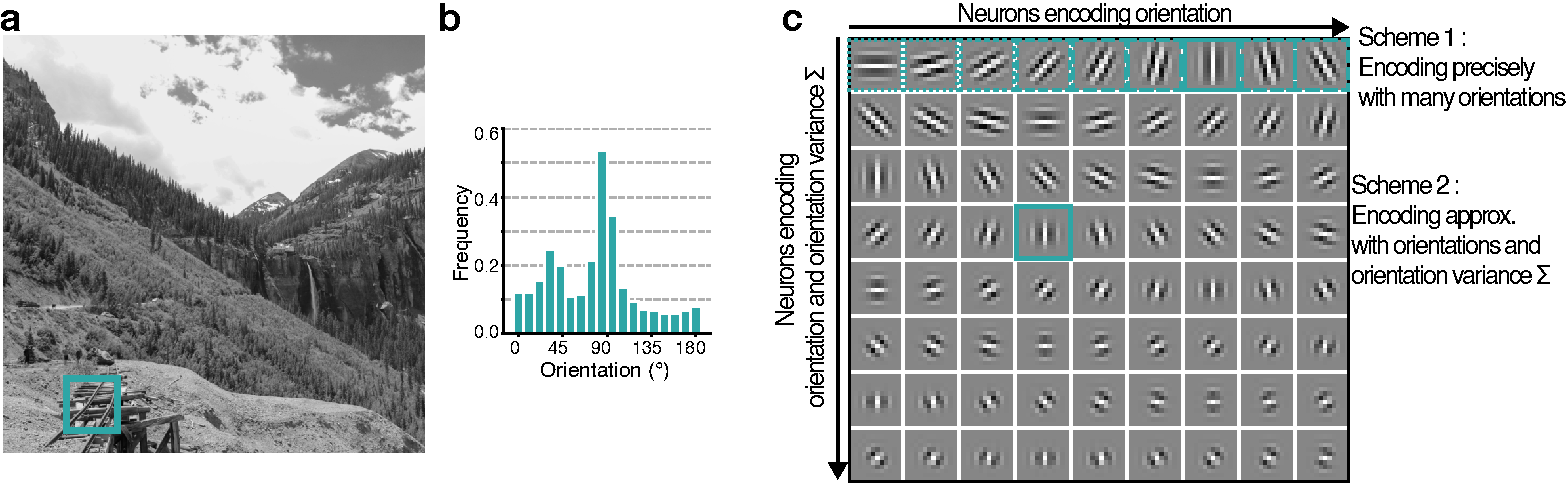
\includegraphics[width=1.\textwidth]{fig/chap3_tradeoff.pdf}
\caption[Sparseness/reconstruction trade-off.]{Sparseness/reconstruction trade-off. (a) A patch of natural image, from the database generated in this article~\cite{ladret2023imgs}. (b) Distribution of orientation from this image, extracted with Sobel filters. (c) Two possible strategies for a neural encoding of this distribution, either through costly but accurate code (Scheme 1) or sparse but less accurate code (Scheme 2).}
\label{fig_chap3_tradeoff}
\end{figure}

This has been preliminarily explored by the Locally Competitive Algorithm, a neuro-inspired algorithm~\cite{rozell2008sparse} which uses recurrent interactions between neurons to drive the sparse coding, as done in Equation~\ref{eq:csc}, but with winner-takes-all competition:
\begin{equation}
    \tau \frac{du_i}{dt} = -u_i + \phi_i - \lambda \sum_{j \neq i} \omega_{ij} \cdot S(u_j) 
\end{equation}
Where \( u_i \) is the internal state (or membrane potential) of neuron \( i \), \( \phi_i \) is the projection of the input onto the \( i^{th} \) basis function (or receptive field), \( \tau \) is a time constant, \( \lambda \) is a positive constant that scales the strength of the competition, \( \omega_{ij} \) represents the degree of overlap or similarity between the receptive fields of neurons \( i \) and \( j \), \( S(u_j) \) is a function that represents the output of neuron \( j \) given its internal state \( u_j \), typically, a threshold function. The design of this algorithm is that neurons compete with each other to represent the input, with neurons that have a dissimilar receptive field competing against one another. Using this Locally Competitive Algorithm as a model of recurrent versus feedforward interactions would also allow seeking which of these two types of connectivity creates the heterogeneous basis functions observed here. It then naturally follows that the next chapter transition from the present functional study, to pinpointing its origin in neurobiological networks.

	\chapter{Encoding of Orientation Variance through Recurrence in V1}

\begin{flushright}
    \textit{''Representations, at a minimum,\\
    must potentially be able to stand in for the things they represent.''}\\
    Chris Eliasmith, How to Build a Brain, 2013
\end{flushright}

\chaptertoc{}



\section{Introduction: Orientation Selectivity in V1}
\subsection{Orientation Selectivity and Representations in the (Visual) Cortex}
As we've largely emphasized so far, orientation selectivity is a hallmark feature of the primary visual cortex. As the first functional element of the visual hierarchy, oriented receptive field form the basis of our understanding of visual processing in the cortex. This is a stereotypical role for a primary sensory cortex, which often exhibit a well-defined invariant feature code (see chapter 3) based on the sensory space they represent~\cite{carandini2012normalization, keller2018predictive}, and acting as the foundation for the downstream computations. For example, the elementary units of voices is neural encoding of tonality and frequency-defined signals~\cite{belin2011understanding}, that of bodily parts is spatially defined segments~\cite{camon2019timing}, and that of vision is our edges of interest, in this manuscript. Examining such foundational elements of image descriptors is a longstanding tradition in the field of visual neuroscience, especially within the framework of hierarchical networks~\cite{van1992information}.

\begin{figure}[h!t]
\vspace{0.1cm}
\centering
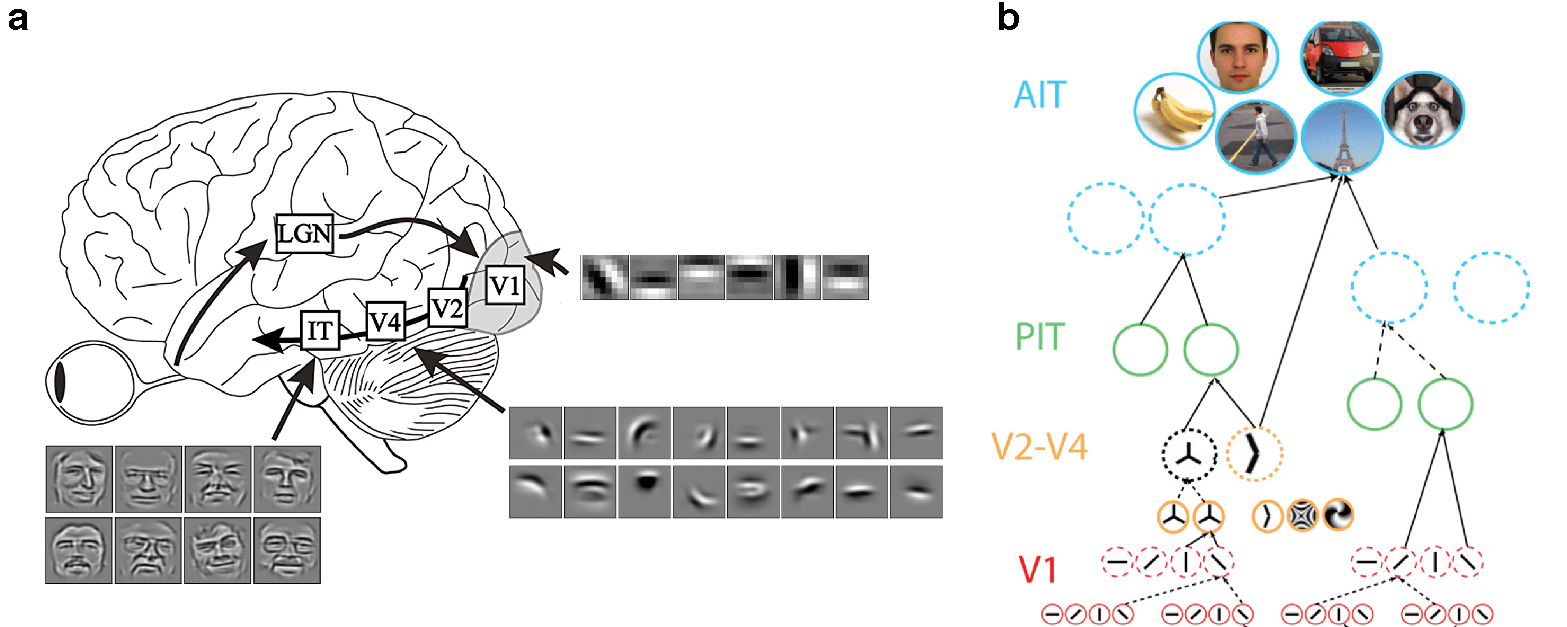
\includegraphics[width=1.\textwidth]{fig/chap4_hierarchical.pdf}
\caption[Hierarchical model of the visual cortex.]{Hierarchical model of the visual cortex (a), oftenmost reflected in the current view of computer vision models (b). Adapted from~\cite{serre2010neuromorphic}.}
\label{fig_chap4_hierarchical}
\end{figure}

In \gls{V1}, the basis of the neural code is a visual one, and has thus the advantage of being easily conceptualized and visualized. This ease-of-understanding of \gls{V1} receptive field, supported by six decades of rich literature, makes orientation selectivity a focal point in of numerous PhD theses, serving either as a principal subject of study or, as is the case here, as an angle of attack to explore theoretical frameworks with testable hypotheses. Most often, this serves to study visual processing as a feedforward model~\cite{kreiman2020beyond}, positing a sequential series of computations wherein basic visual components like edges are integrated to form progressively complex representations such as angles, textures, and eventually high-level objects, as observed in different visual cortical areas (V1, V2, V4, IT)~\cite{lamme1998feedforward}. The feedforward model proposes a structured pathway through which visual information is processed and refined at each subsequent level, contributing to a global, coherent perception of the visual world, as shown in Figure~\ref{fig_chap4_hierarchical}. For the sake of argumentation of this thesis, this view can be advantageous. Hierarchical modelling requires that separate features will be processed in separate areas, and as such, separate feature variances to be also localized and confined within each cortical area.

A notable limitation of the feedforward model lies in its inability to effectively distinguish between perceptions driven by bottom-up sensory input and the self-generated sensory feedback resulting from an organism's actions~\cite{von1950reafferenzprinzip,keller2018predictive}. In the case of vision, the visual flow stemming from eye movements could trigger an optokinetic reflex, akin to the reflexive response which stabilizes our view as we are reading this manuscript. Should an organism fail to discern between external and self-generated inputs, this reflex would inhibit any eye movement. As such, it follows logically that visual processes must also contain some form of feedback.
A simplistic strategy to mitigate this issue could be simply cancelling the predictable consequences of self-generated sensory feedback, by sending an efference copy of a motor command. 
Conceptually, such transformative processes require an internal model, can be viewed as equivalents to a simulation of the external world and its consequences for the organism. In a rather simple way (Figure~\ref{fig_chap4_representational_framework}), this extends the general feedforward representation framework into a predictive one, as used in this thesis~\cite{friston2016active}.

\begin{figure}[h!tbp]
\vspace{0.1cm}
\centering
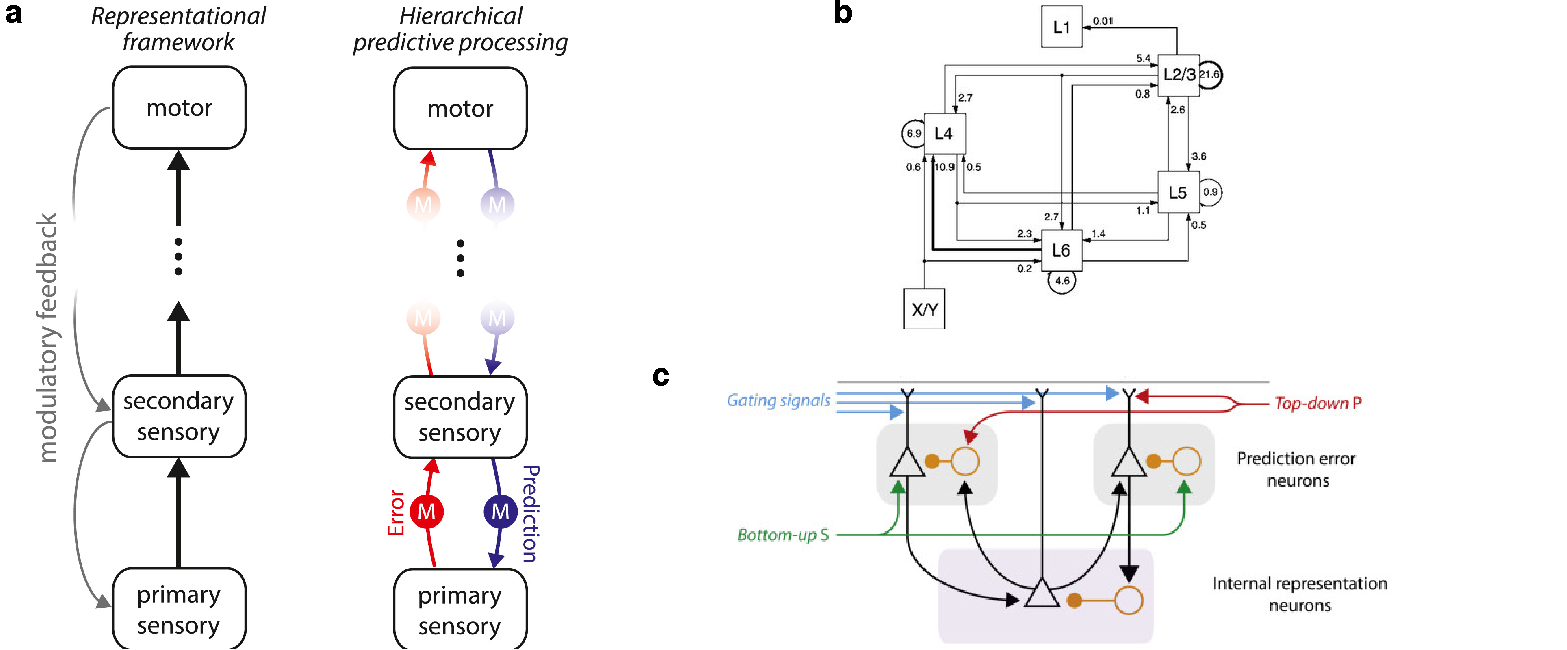
\includegraphics[width=1.\textwidth]{fig/chap4_representational_framework.pdf}
\caption[Representational and predictive frameworks.]{Representation and predictive frameworks in neuroscience. (a) Predictive coding extends the classical representational framework with the addition of prediction and related error neural elements. At the relevant level of scale here, this extends the canonical microcircuit~\cite{douglas1989canonical} (b) into a predictive neural circuit (c). Adapted from \cite{douglas1989canonical} and~\cite{keller2018predictive}.}
\label{fig_chap4_representational_framework}
\end{figure}

Although this doesn't challenge the notion that orientation selectivity is an optimal feature for a model of vision, it does offer an alternative perspective for the present chapter. Our aim here is to illustrate that, within a predictive modelling framework, \gls{V1} neurons don't just represent a singular feature, but also its variance, encoding a probabilistic distribution that form parts of a generative model.



\subsection{The Origin of Orientation Selectivity in the Cortex}
Pinpointing the origin of an invariant representation of images implemented within a biological neural network is a non-linear and non-trivial task. As such, there are as many theories related to "how" orientation selectivity emerges as there are theories as to "why" it exists. While it is impossible to make an exhaustive list of all phenomenological accounts and their myriad of variations, they can be grouped in three aspects:
\begin{itemize}
    \item Orientation selectivity emerges through converging, feedforward interactions.
    \item Orientation selectivity is refined by local (i.e. within a cortical area) recurrent, horizontal interactions.
    \item Orientation selectivity is modulated by extrastriate feedback interactions. 
\end{itemize}
As is the case with many complex biological questions framed as multiple choice, the answer is "all of the above, mixed non-linearly" (Figure~\ref{fig_chap4_vidyasagar}).

\begin{figure}[h!tbp]
\vspace{0.1cm}
\centering
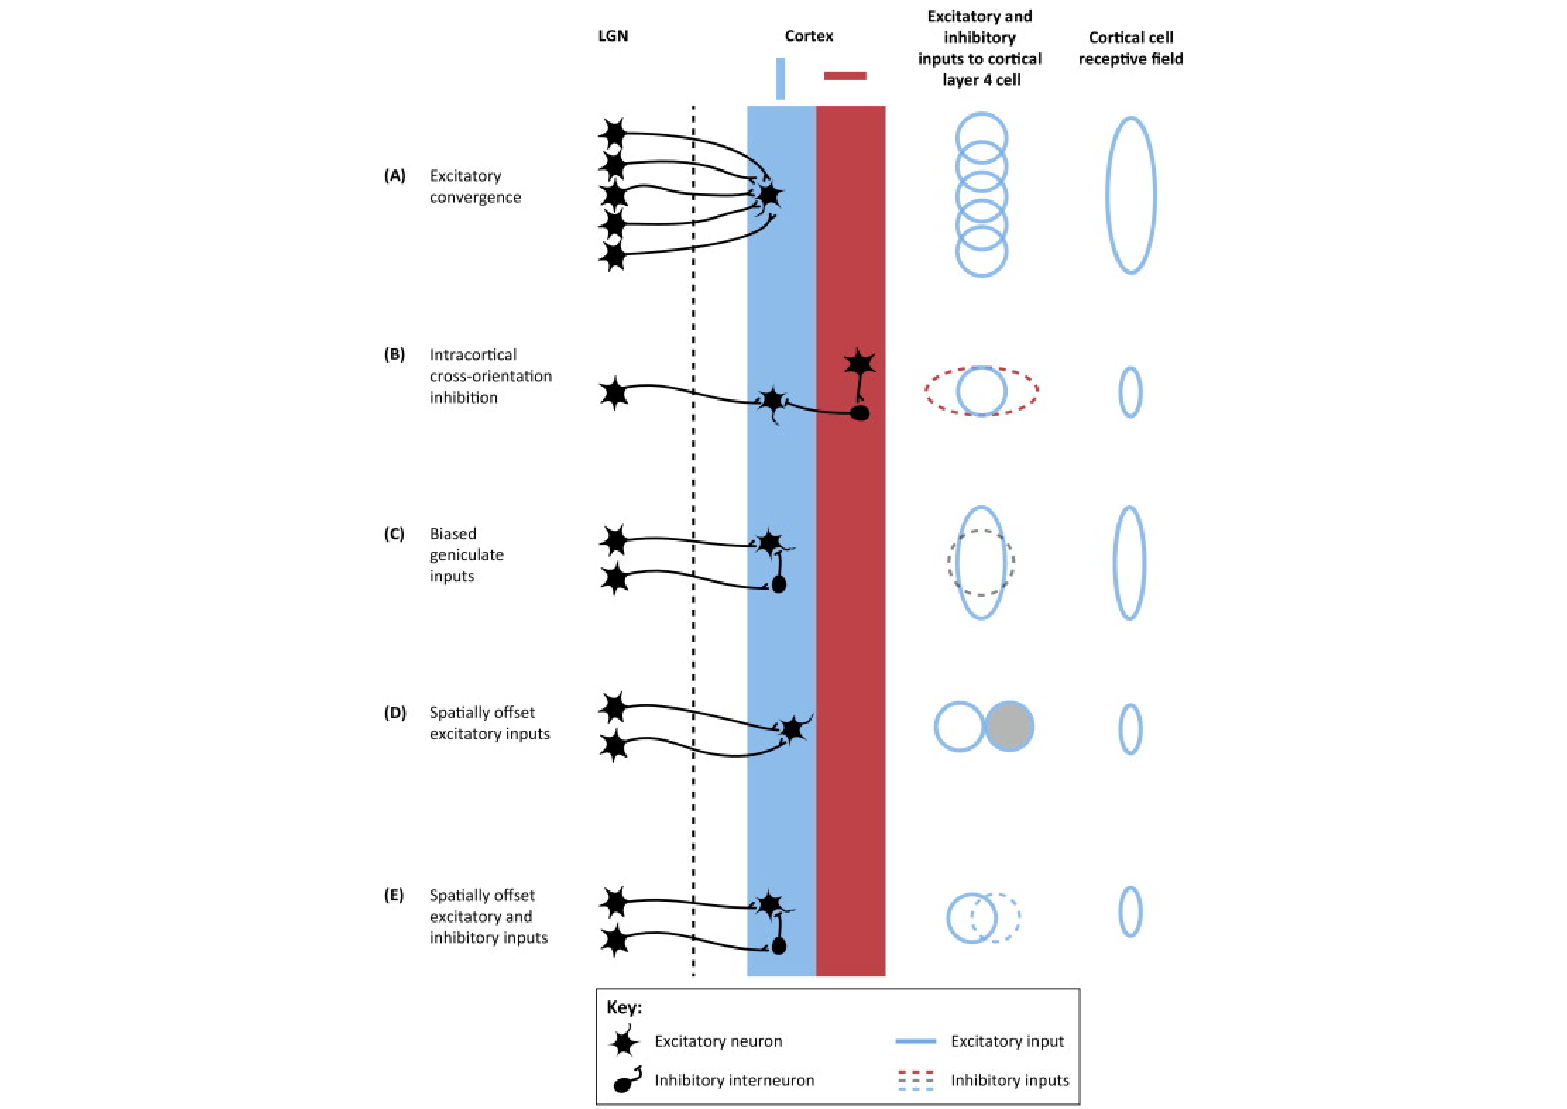
\includegraphics[width=.8\textwidth]{fig/chap4_vidyasagar.pdf}
\caption[Possible mechanisms for orientation selectivity.]{Possible mechanisms accounting for the existence of orientation selectivity, reproduced from~\cite{vidyasagar2015origins}.}
\label{fig_chap4_vidyasagar}
\end{figure}

The feedforward explanation for the emergence of orientation selectivity aligns intuitively with the feedforward representational framework discussed earlier. This "canonical" model, as introduced by Hubel and Wiesel in their seminal work~\cite{hubel1962receptive}, frames orientation selectivity as arising from the convergence of isotropic receptive fields from the \gls{LGN} to \gls{V1}. While this has been validated experimentally several times~\cite{ferster1986orientation, chapman1991relation}, such studies fail to explain the presence of (minor) orientation tuning before \gls{V1}. Specifically, when cortical networks are silenced to exclusively observe \gls{LGN} input to \gls{V1}, the resulting input is already sharply orientation-tuned~\cite{ferster1996orientation}. 
This could stem from the fact that some \gls{LGN} cells are already slightly tuned to orientation, perhaps through a certain degree of retino-\gls{LGN} convergence~\cite{xu2002primate,tan2011orientation,van2013transformation}. Indeed, even with a single thalamic oriented neuron, it is possible to obtain an excitatory orientation-tuned response in a connected \gls{V1} neuron~\cite{kara2002spatial}. 

\begin{figure}[h!tbp]
\vspace{0.1cm}
\centering
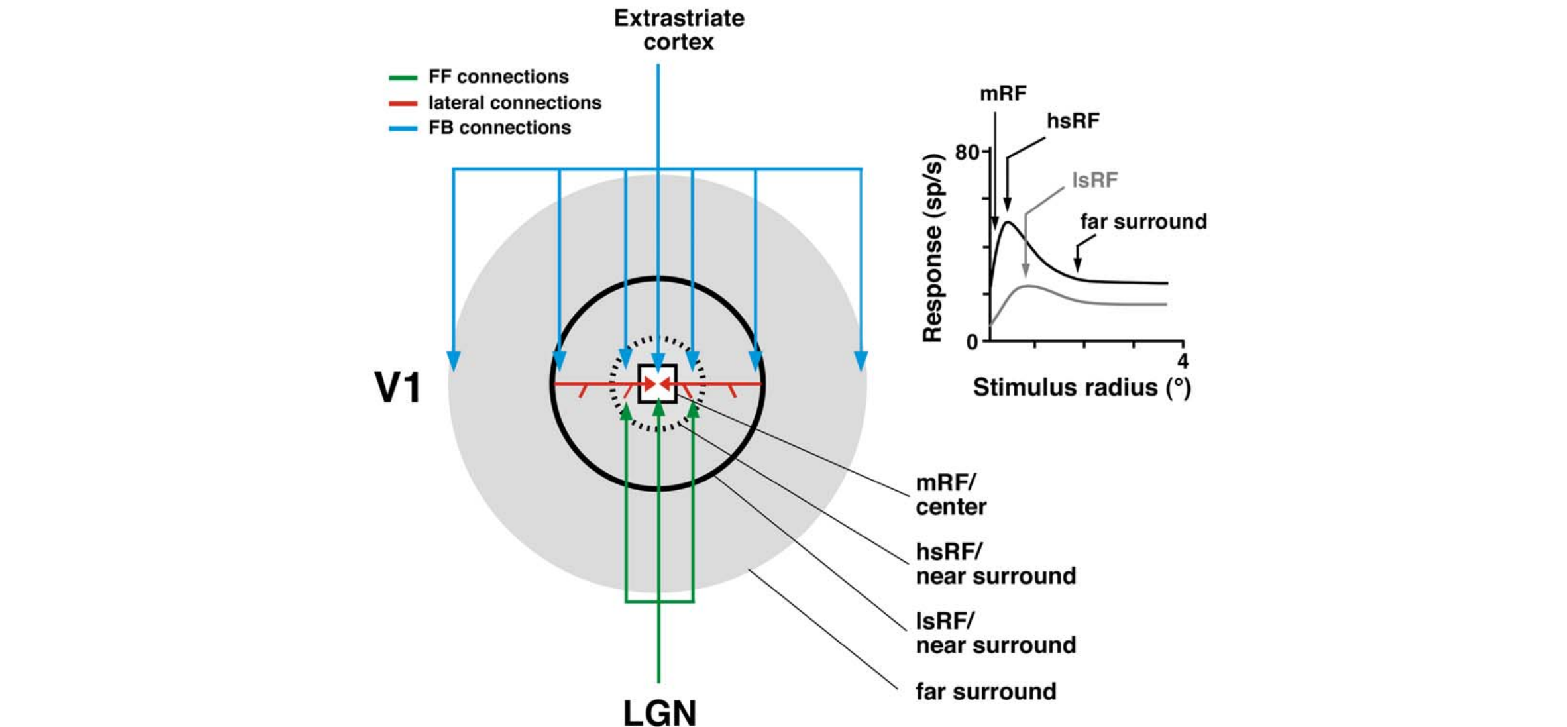
\includegraphics[width=1.\textwidth]{fig/chap4_angelucci.pdf}
\caption[Spatial extent of \gls{V1} connections.]{Spatial extent and response induced by feedforward (FF), lateral and feedback (FB) connections. Adapted from~\cite{angelucci2006contribution}.}
\label{fig_chap4_angelucci}
\end{figure}

This feedforward account of orientation selectivity is typically contrasted to the intracortical recurrent hypothesis. At the meso-scale of \gls{V1}, orientation selectivity is arranged in a "map", where neighboring neurons have heterogeneous preference~\cite{grinvald1986functional}. Long-range horizontal axons have been reported to preferentially bind to distant columns of similar orientation preferences in the cat \gls{V1}, with short-range recurrent connectivity being more heterogeneous~\cite{chavane2011lateral, chavane2022revisiting}. This would allow having interactions between neurons tuned to different orientation at short range, as we will put forward in the present article, whilst maintaining the possibility to prime contours made of similar orientation at long range. Cross-orientation inhibition within the cortex can theoretically perform orientation sharpening~\cite{priebe2012mechanisms}. This could either be responsible, on its own, for generating orientation selectivity~\cite{hansel2012mechanism}, or could serve to refine the feature emerging from the feedforward convergence. Additional mechanisms encompass voltage-sensitive mechanisms with precise location within the dendritic tree, but also intracortical excitation emanating from cells that are tuned to analogous orientations ~\cite{vidyasagar1996multiple, priebe2012mechanisms,vidyasagar2015origins}.

This also yields an interesting counter-observation, given that precisely organized orientation maps are solely present in \gls{V1} of carnivora and primates~\cite{jang2020retino}. Rodent, on the other end, have a "salt-and-pepper" (random) topology of orientation detectors, with no specific spatial mapping onto the cortex. However, through a delicate balance of excitation and inhibition, it is also possible that these networks recurrently create orientation selective neural activity~\cite{hansel2012mechanism}. This is corroborated by the notion that recurrent interactions among potentially isotropic cortical neurons can yield properties akin to those arising from feedforward interactions. In other terms, this implies that functional convergence, whether feedforward or recurrent, is an inherently viable mechanism for the emergence of orientation selectivity. Extending this idea, one can also think of the complex cells (see Introduction 2.1.1.2.) as either a convergence of simple cells, but also as recurrently "amplified" simple cells~\cite{chance1999complex}.



Given that these rodents also exhibit orientation tuning within the \gls{LGN}~\cite{tan2011orientation}, this raises additional questions. Do these phenomena reflect unique characteristics specific to certain species, or do they suggest a more comprehensive need to re-evaluate established beliefs about orientation selectivity? This question becomes especially pertinent when we consider the wide range of species exhibiting pronounced orientation tuning within the cortex. This possible difference in strategy for orientation selectivity might also speak of different strategies for processing associated variance, between primates, cats and mice. As we shall see at the end of this chapter, primates and cats seemingly exhibit similar behavior, but recordings on mice are currently underway in our laboratory, and will be discussed in the Conclusion of this thesis. 

\begin{figure}[htbp]
\vspace{0.1cm}
\centering
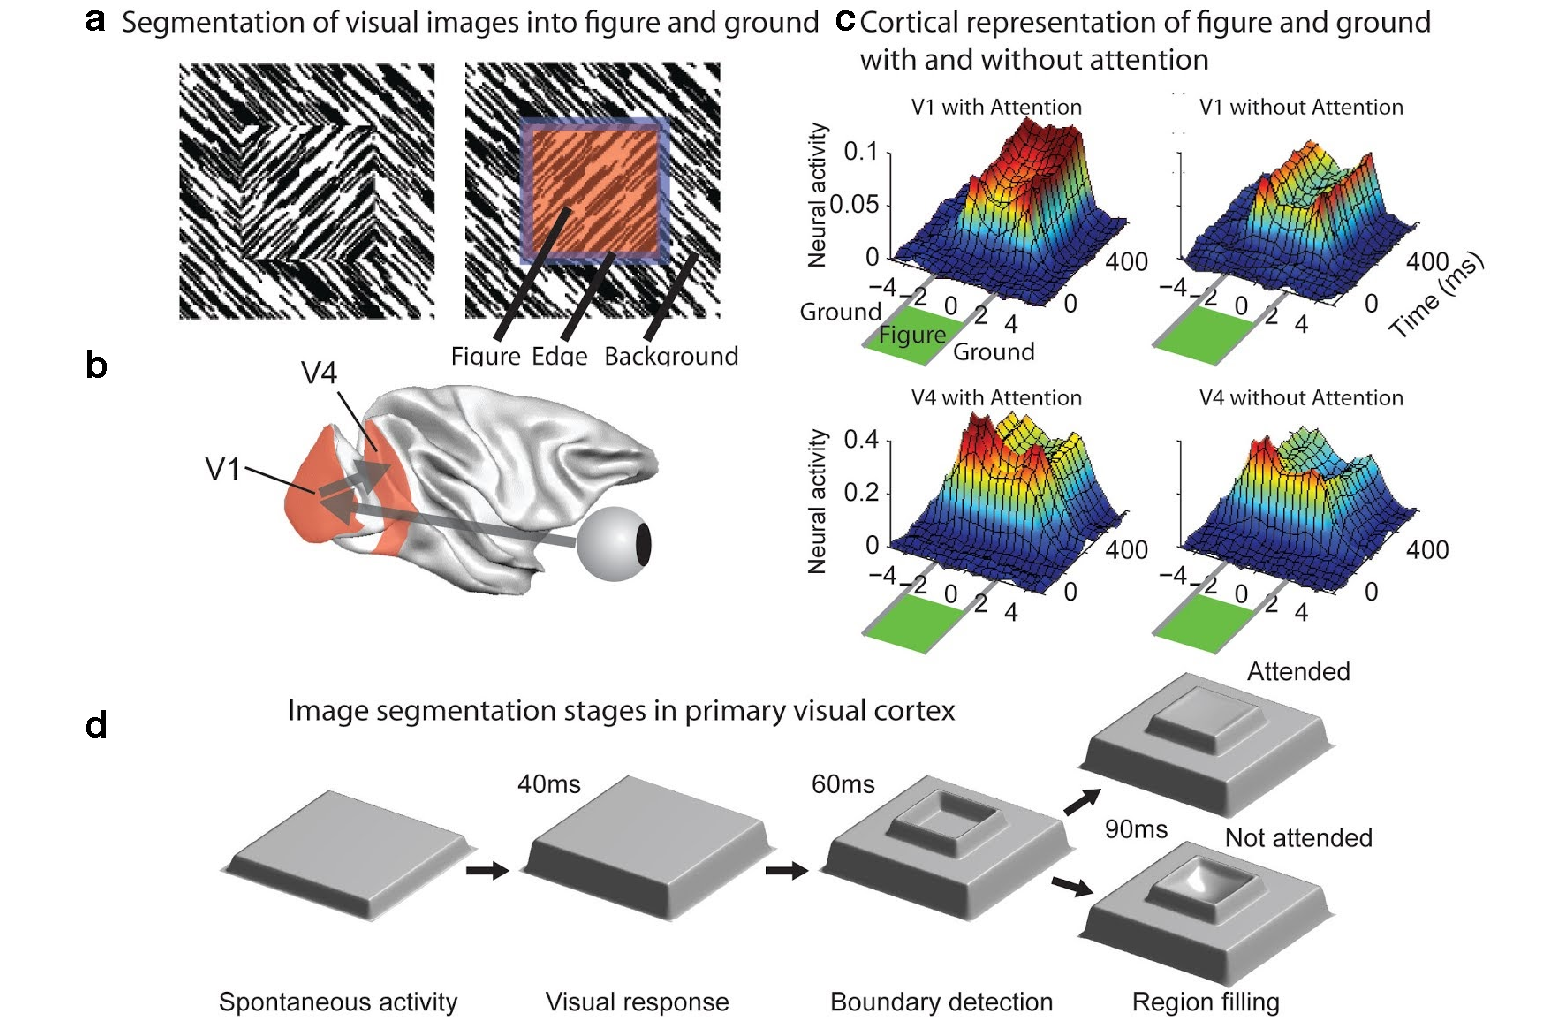
\includegraphics[width=1.\textwidth]{fig/chap4_roelfsema.pdf}
\caption[Feedback modulation of \gls{V1} activity.]{Feedback from extrastriate areas modulates \gls{V1} orientation selectivity. (a) In a task of segmenting various elements in a naturalistic context, (b) both orientation selectivity and texture selectivity, from \gls{V1} and V4 respectively, are involved. (c) The receptive field of \gls{V1} neurons changes with attention towards the figure, which is based on feedback from V4, as summarized in (d). Figures reproduced from~\cite{poort2012role}}
\label{fig_chap4_roelfsema}
\end{figure} 

Finally, \gls{V1} receives substantial and potent feedback from extrastriate cortical areas, which plays a pivotal role in shaping orientation selectivity. A salient illustration of this intricate relationship is observed in the task of figure-ground segmentation: the feedback from extrastriate areas (here, V4), allows \gls{V1} to not only to delineate the edges with precision, but also to a fully-fledged figure in meticulous details~\cite{poort2012role} (Figure~\ref{fig_chap4_roelfsema}). This feedback exhibits a broader spatial extent compared to the feedforward receptive field, adding a layer of complexity to our understanding~\cite{angelucci2006contribution}.

In predictive coding terms, such feedback mechanisms are modeled as carrying the predictions from higher-order regions to \gls{V1}. It is often implied by predictive coding these feedbacks should be modulatory only~\cite{bastos2012canonical}, in order to send prediction from higher- to lower-order areas that can suppress prediction errors produced by bottom-up input. This is however neither true~\cite{murphy1987corticofugal,wozny2011specificity, covic2011synaptic} nor required, as mixed excitatory/inhibitory influence can mediate the construction of prediction and prediction errors locally. The modular nature of this activity will be discussed further in the next chapter.

Overall, one can see how orientation selectivity in \gls{V1} is a well-defined invariant representation of low-level features of the world. As such, it serves as the perfect predictions of these features, and hence, is constrained to variance weighting, as developed in Equation~\ref{eq_pc_matrix}. While there is no clear consensus on the origin of orientation selectivity in \gls{V1}, there is no debate that the cortical circuitry is dedicated to maintain it, through a complex mix of many neural activities, that must be first recorded and then deciphered to the best of the experimenter's ability.



\section{Methods: Visual Electrophysiology and Neural Decoding}
\subsection{Recordings Tools of the Brain}

\begin{figure}[h!tbp]
\vspace{0.1cm}
\centering
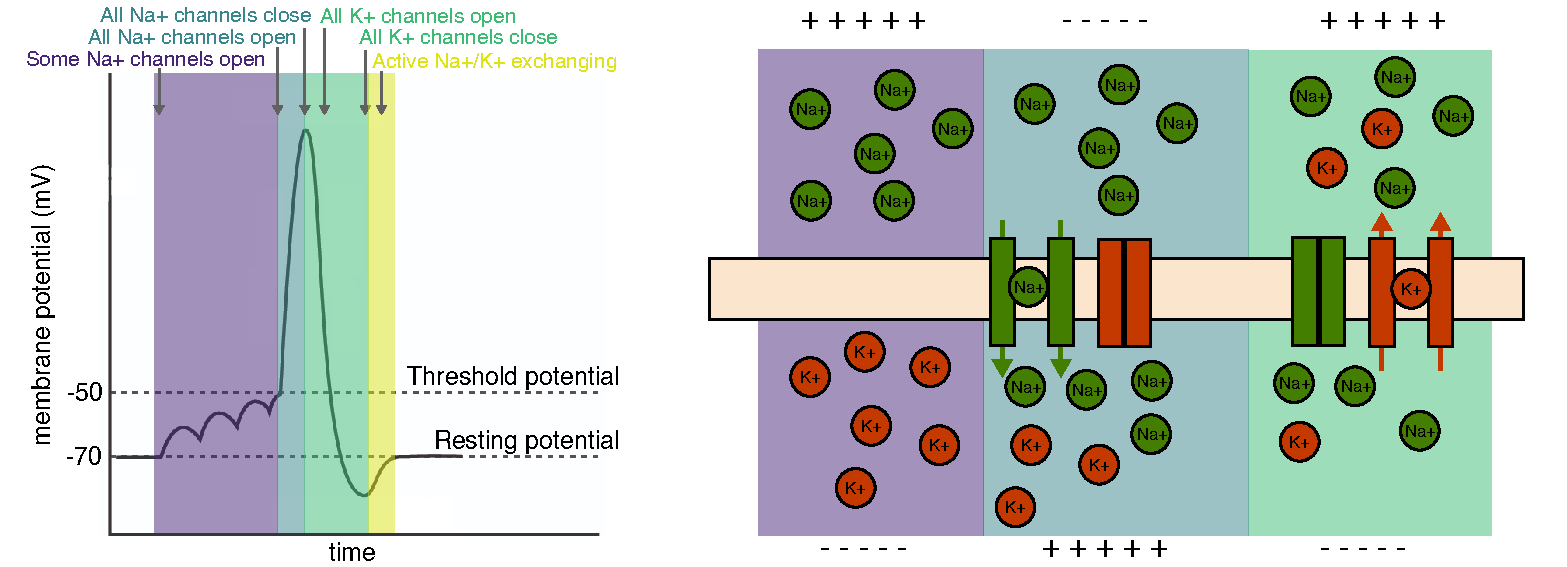
\includegraphics[width=1.\textwidth]{fig/chap4_actionpotential.pdf}
\caption[Illustration of the action potential.]{Schematic illustration of the action potential on the membrane potential (left) and its respective ionic currents (right). The final active Na+/K+ exchanging is not illustrated.}
\label{fig_chap4_actionpotential}
\end{figure} 

Neurons, as the functional units of the nervous system, communicate through sophisticated electrochemical activity, which involve using the flow of ions to generate electrical gradients~\cite{kandel2000principles}. To simplify this process, neurons effectively maintain an electrochemical gradient that puts them at an electric potential of $-70$mV with respect to their local environment. Upon binding of a neurotransmitter, channels specifically let Na$+$ ions flow through, depolarizing the neurons up to approximately $+40$mV. The neuron then activates energy-consuming K$+$ channels, re-establishing a polarized electrochemical gradient, with a slight overshooting. This change of activity propagates from the neuron's soma to its axon terminal, where it induces the fusion of synaptic vesicles through the entry of Ca$2+$ ions, resulting in the release of neurotransmitters into the synaptic cleft, which in turn can alter the conductance of the post-synaptic neuron (Figure~\ref{fig_chap4_actionpotential}). The modulation of conductance in the post-synaptic neuron is crucial as it may lead to the generation of a new action potential, thus perpetuating the chain of neural communication.

% figure recording techniques from isabelle's thesis https://www.spiedigitallibrary.org/journals/neurophotonics/volume-4/issue-03/031215/Improving-voltage-sensitive-dye-imaging--with-a-little-help/10.1117/1.NPh.4.3.031215.full?SSO=1
\begin{figure}[h!tbp]
\vspace{0.1cm}
\centering
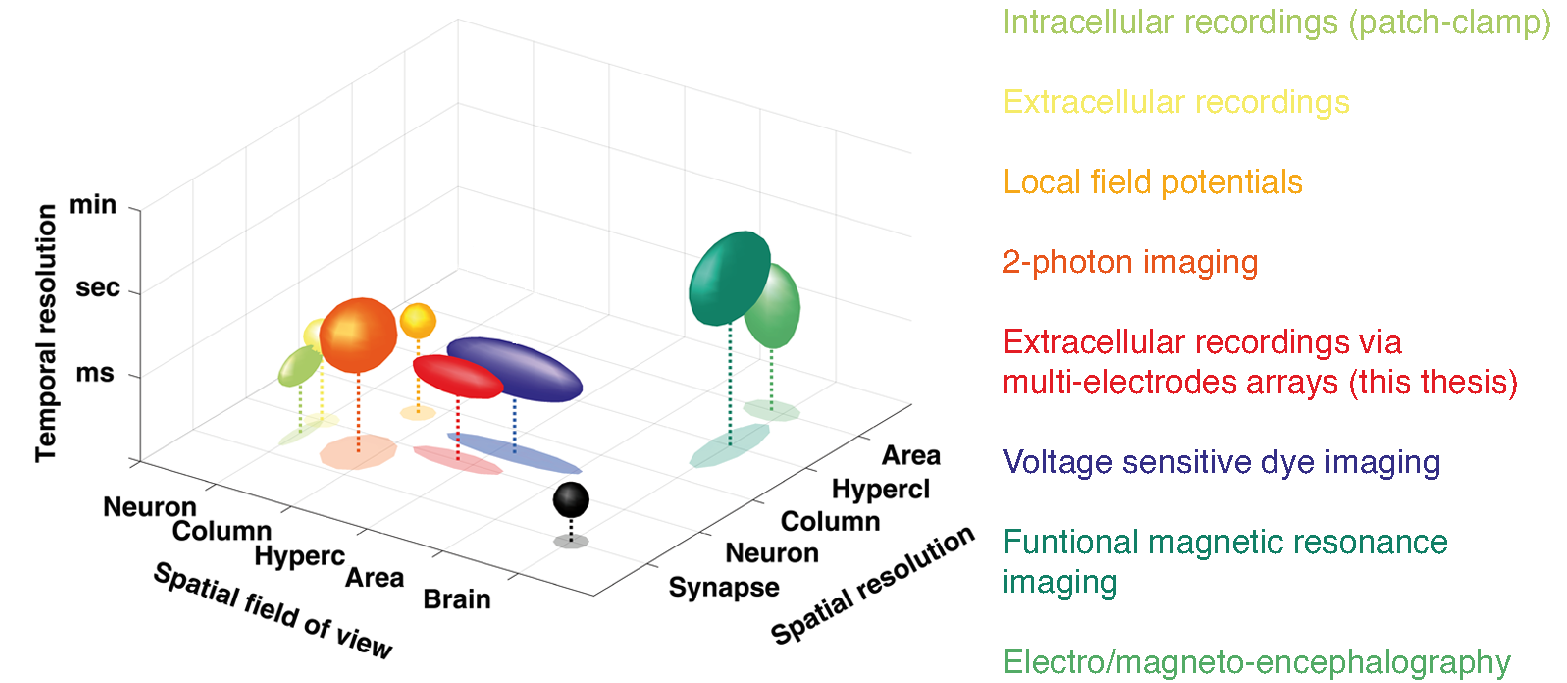
\includegraphics[width=1.\textwidth]{fig/chap4_chemla.pdf}
\caption[Methods of recording of the central nervous system.]{Spatial field of view, and spatio-temporal resolution of various methods of recordings of the nervous system, from~\cite{chemla2010voltage}.}
\label{fig_chap4_chemla}
\end{figure} 

This mechanism, (over)simplified here for clarity's sake, forms the basis of neural communication. Thus, all methods employed for recording brain activity are inherently also based on it. The lowest possible level (in terms of spatial and temporal resolution) of such recording methods consists in approaching a glass pipette with an electrode to the membrane of the neuron, then forming a seal to directly record that patch of membrane~\cite{sakmann1984patch}. This allows to record single ionic channels, which is highly effective for mapping conductance of ion to single molecules. By breaking this seal, it is possible to record the whole neuron, but also control its dynamics using current or voltage injection. Whether at the single channel or membrane level, such methods are known as "patch-clamp"~\cite{neher1992patch}, either in "current-clamp" or "voltage-clamp" mode. 

\begin{figure}[h!tbp]
\vspace{0.1cm}
\centering
\includegraphics[width=1.\textwidth]{fig/chap4_multielectrodes.pdf}
\caption[Extracellular electrodes.]{Various types of extracellular electrodes, with cortical slice of mouse visual cortex (acquired by Geneviève Cyr) for size reference. }
\label{fig_chap4_multielectrodes}
\end{figure} 

Patch-clamp techniques, while allowing to measure single neuron activity in exquisite details, cannot record from populations of neurons. Consequently, for questions related to the internal representations of certain features with an ensemble of neural activity, it is often best to measure electrical potential variations outside the neuron, which does not involve precisely putting an electrode on the neuronal membrane~\cite{buzsaki2012origin}. Rather, this method necessitates the insertion of electrodes into the brain, a procedure historically done using tungsten electrodes~\cite{hubel1959receptive, garrido2022understanding}, but nowadays predominantly achieved using multi-channel electrodes made from complex alloys~\cite{csicsvari2003massively}. This method of recording is the one used throughout this thesis (Figure~\ref{fig_chap4_multielectrodes}).

Multi-channel electrodes permit the recording of electrical activity from a multitude of neurons simultaneously, allowing extensive data collection and nuanced understanding of neural dynamics~\cite{steinmetz2018challenges,steinmetz2021neuropixels}. As of 2023, the advanced state of this technology allows for the recording of approximately one thousand neurons concurrently. Presently, we employed electrodes with lower channel counts, specifically $32$ to record neural activity. The spatial configuration of these electrodes is varied, but typically that of a linear probe, with contacts all along the vertical axis of the probe. In chapter 5, we will use a grid-like variation of that probe, which does not allow to probe for layer-specific computations, but for horizontally distributed ones instead.
Signals recorded by extracellular electrode are a mixture of activity from multiple currents and neurons near each electrode site. To assign each extracellular event to a given neuron, several algorithms exist, each performing a different (but related) version of a "spike-sorting" process. Here, Kilosort3~\cite{pachitariu2016kilosort, rossant2016spike} is used, which performs template-matching based on the extracellular events' waveforms, and has been shown to achieve state-of-the-art performance for multi-channel electrodes. Nonetheless, its output requires a (lengthy) post-processing step by the experimenter, to merge and dissociate entangled neuronal activity, which is here done with a graphical interface called "Phy"~\cite{rossant2016spike}. 

Depending on the frequency at which the signal is filtered, one can also record the local field potential from these electrodes. This constitutes a non-assigned, summed signal of all neuronal activity from neighboring units~\cite{kajikawa2011local,herreras2016local}. This technique is quite useful, because by recording the polarities of the events, one can observe the "sink" of neural activity arriving after a visual a stimulation in the layer IV of \gls{V1}, and the corresponding "source" in deeper and upper layers~\cite{schaefer2015quantification}. These sink/source terms refer to the influx of Na$2+$ ions (creating a "sink" outside the neurons) after a depolarization, and inversely for the "source". This technique is used in the present article to assign a cortical layer to the recorded neurons~\cite{ladret2023cortical}.

For the sake of a comprehensive overview, let us continue exploring the various recording tools of the brain. As far as neuron counts is concerned, increases in scale then require a change from electrodes to optical recording methods. A notable example that drives many experiments at the time of writing is calcium imaging, a technique driven by the principle that $Ca2+$ influx related to an action potential~\cite{stosiek2003vivo,friedrich2017fast}. This method enables the simultaneous recording of the activities of tens of thousands of neurons~\cite{stringer2019high}. However, its application is hampered by depth limitations, owing to the inherent constraints of optical tools in penetrating the depth of the cortex. To overcome this limitation, the exploitation of advanced physical phenomena such as two- or three-photon effects can be employed, allowing for increased depth of imaging~\cite{cheng2011simultaneous}. However, this entails a surge in the complexity of the acquisition system. The implementation of this technique also necessitates unobstructed optical access to the cortex, involving the removal of the skull for acute experiments and, in some cases, its substitution with viewing glass for chronic studies. The temporal resolution of the calcium imaging is on the scale of tens of milliseconds, which can hide single-neuron dynamics. To that end, there exists the possibility of loading the cortex with Voltage-Sensitive Dye (VSD), which loads the cortical areas with a molecule sensitive to changes in voltage~\cite{chemla2010voltage}. This technique grants superior temporal resolution~\cite{chemla2010biophysical}, allowing for detailed imaging across the entire cortical area, but most importantly, sub-action potential recordings, because it does not rely on the Ca$2+$ influx of the action potential.

At the culmination of the spectrum of recording methodologies are macroscale recordings, which encompass a range of diverse techniques, each providing unique and non-invasive insights into brain activity. Direct measurements of electrical activity can be obtained through the widely known Electroencephalography (EEG)~\cite{millett2001hans}, which measures the sink/source currents of the large cortical pyramidal neurons, offering insights into the global electrical activity of the brain~\cite{kirschstein2009source}. This is, in a way, the extra-cranial version of the recordings of Local Field Potentials described above. For finer resolution, one can rely on Magnetoencephalography, a sophisticated method that records the orthogonal magnetic field corresponding to the electrical signals generated by neural activity~\cite{hansen2010meg}. The acquisition setup is however significantly more complex, necessitating the integration of supra-conductive sensors to precisely capture the delicate magnetic fields associated with neural currents. Lastly, the mainstream method for large-brain analysis is functional Magnetic Resonance Imaging, a technique that detects the magnetic signatures of oxygen-binding molecules~\cite{worsley1995analysis,logothetis2008we}. These molecules flow into specific regions of the brain in response to neural activity to restore the local energy supply to neurons~\cite{phillips2016neurovascular}. By mapping these blood flow changes, this technique enables the indirect observation of neural activity, providing (rough) insights into the functional organization of the brain

Each of these techniques, despite their complexities and inherent limitations, contributes uniquely to our expansive view of neural activity, providing distinct insights into the dynamic interplay of neural circuits. These advanced methodologies, in conjunction with continuous advancements in neuroscientific research, are instrumental in unraveling the intricate tapestry of neuronal interactions and communications.

\subsection{Making Sense of the Recordings}
It may appear straightforward to correlate a single visual input with the quantity of spikes discharged by a single neuron and call it a code. However, this seemingly straightforward approach, formally called  "rate coding", involves the prior that the frequency of spike emissions by a neuron is presumed to signify its sensitivity to a particular stimulus. Under this paradigm, a higher spike rate is interpreted as indicative of greater neuronal responsiveness to the stimulus. As we have detailed in the introduction, this assumption stands in contrast to substantial evidence suggesting that neurons inherently strive to minimize their energy consumption as much as possible. The rate-based model, although used by Hubel and Wiesel in the original orientation-selectivity articles~\cite{hubel1959receptive, hubel1962receptive}, does not capture the full breadth of possible information strategies contained in neural recordings. 

Navigating through all the intricate mechanisms of neural coding could mandate an extra dedicated manuscript. However, the main alternative hypothesis to rate coding is temporal coding~\cite{engel1992temporal}, which posits that neurons encode information through intricate patterns in the timing of their spikes, implicating diverse aspects such as delays~\cite{grimaldi2022precise}, synchronicity, and first-spike times in the encoding process.
These multifaceted strategies all imply a different way to look at the data. This can be manageable for recordings with a low neuron count, such as an implanted electrode in a given area for an extended period of time~\cite{nougaret2023distinct}. With great sampling power comes little understandability, and with experiments with hundreds of neurons, it becomes harder to disentangle the meaning from the noise in the recordings. This is where machine learning-based approaches come in, allowing the experimenter to study its recordings with minimal prior assumptions.

\begin{figure}[h!tbp]
\vspace{0.1cm}
\centering
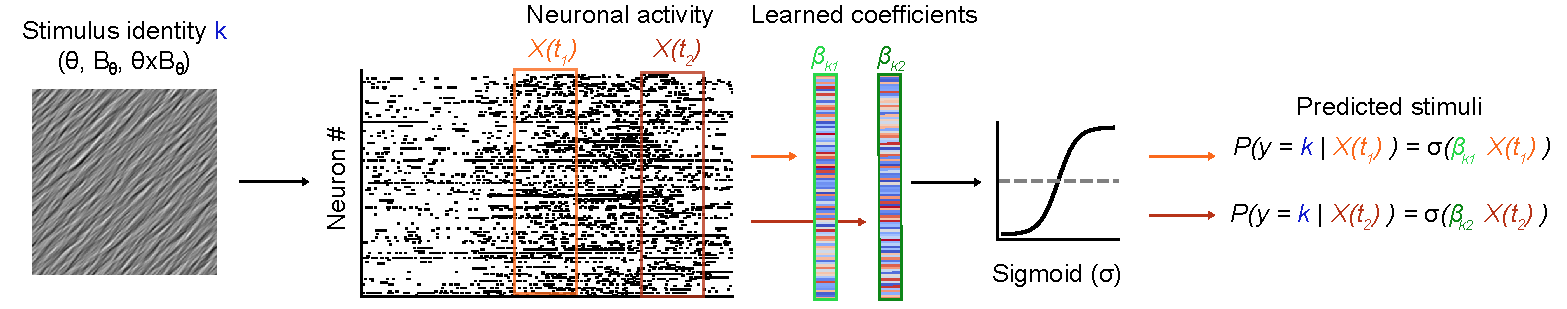
\includegraphics[width=1.\textwidth]{fig/chap4_logreg.pdf}
\caption[Illustration of logistic regression applied to neuronal decoding.]{Illustration of logistic regression applied to neuronal decoding. Additional details on the mathematical framework can be found in the chapter's article.}
\label{fig_chap4_logreg} % copy paste from previous article
\end{figure} 

As the sensory organs can essentially be seen as "encoding" the features of the world, using machine learning (or really, any non-computationally trivial) techniques to understand the neural activity is referred to as "neural decoding"~\cite{meyers2013neural,glaser2020machine}. Numerous approaches exist for neural decoding, mostly aiming to categorize neural activity into distinct types of stimuli through labelled, supervised training. The efficacy of a decoding algorithm is contingent upon its ability to discriminate between different types of neural activity; the more refined the discrimination, the more accurate the encoding of the feature to be classified within the neuron. Intuitively, this is akin to having a better separate of two conditional distributions in the neural substrate, which yields better classifier performance as the boundary between these distributions becomes better defined. For a given algorithm with optimal parametrization, improvement of the classification based on two different recordings means that features sought-after in the recordings have become more disentangled by the neurons in feature space~\cite{bishop2006pattern}. 

This forms the basis of the present article. In this research, we employ logistic regression as our neural decoder, a method praised for its simplicity, efficiency, and biological plausibility. While the implementation details are elaborated within the article, the foundational principle is depicted in the accompanying figure above. Logistic regression serves as a robust tool to unravel the complex patterns within neural datasets, allowing for the elucidation of the nuanced interactions and responses of neurons to varied stimuli.





\section{Article: "Cortical Recurrence supports Resilience to Sensory Variance in the Primary Visual Cortex"}
The following article represents a key contribution of this thesis, notably by introducing two novel neuronal responses that contribute to sensory variance encoding. Using a computational model, we validate these findings through a computational model of intracortical connectivity, which serves as the cornerstone for our argument as to how the brain processes distributions of naturalistic inputs in subsequent chapters.\\ 

Full citation is as follows: \fullcite{ladret2023cortical}
% avant d'intégrer un article dans votre thèse, consulter http://www.sherpa.ac.uk/romeo/ si vous souhaitez diffuser sur internet
\includepdfset{pagecommand=\thispagestyle{scrheadings}} % ajoute la numérotation continue des pages aux fichiers pdf importés
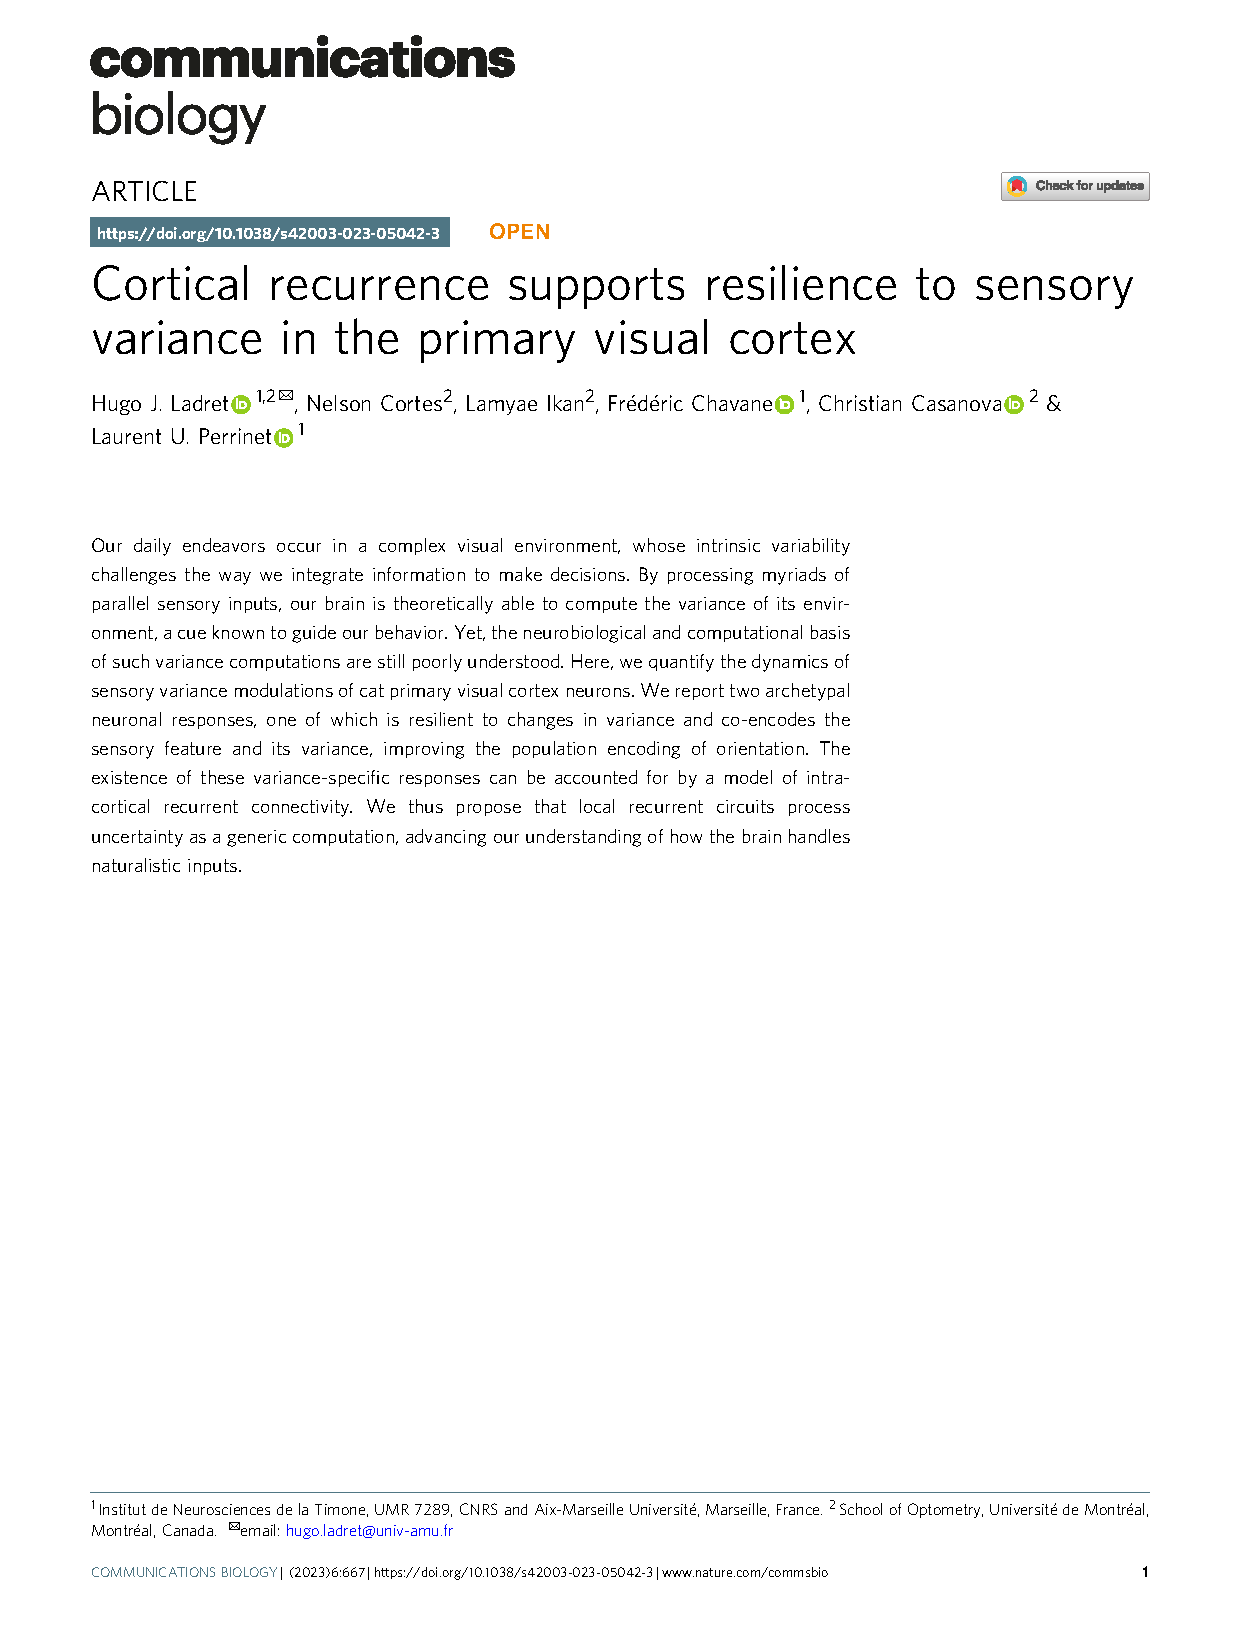
\includepdf[scale=0.82,pages=-]{papers/natcomsbio.pdf} % 'scale' ajuste la taille du pdf, vous pouvez affiner en fonction des marges




\section{Conclusion}
In this article, we have studied how the (inverse) variance of oriented inputs affects \gls{V1}. We have replicated some neural responses known in macaques\gls{V1}~\cite{goris2015origin}, extending them to complex modulations of the dynamics of single neurons and populations. Using a prior-free machine-learning approach, we have probed for neural code in the population activity, uncovering two functional types of neurons that can encode either solely the sensory feature, or jointly the sensory feature and its variance. Based on cortical layer position and on a computational approach, we propose that the processing input variance in \gls{V1} is supported by recurrent connectivity between local cortical populations.

This directly ties the present article into the predictive processing framework introduced earlier in the manuscript (Equation~\ref{eq_proba_intro}), as the experiments here essentially mean consists in manipulating the variance $\Sigma_u$ of a light pattern, in combination with its mean $g(v)$, respectively $B_\theta$ and $\theta$ in the article. While this means total access over the distribution of the input, two limitations on the predictive aspect of these recordings are missing. First, the distribution of internal priors were not controlled, for tractability's sake. This could have been done with an adaptation protocol, for example, by biasing the input over a given set of variables~\cite{damasse2018reinforcement}. Second, we did not control whether the recorded neurons were encoding prediction errors or predictions. The former is rather simple to do, by inducing a mismatch between an unexpected sequence of patterns~\cite{keller2012sensorimotor} (for example, an abrupt change of repeated orientations). The latter is more complex, as a major challenge in identifying them stems from their propensity to response like bottom-up activated neurons in various conditions~\cite{keller2018predictive}. 

Nonetheless, the present results provide an experimental validation of probabilistic processing in the brain, if not directly predictive (due to the anesthetized setup). This proves that there exists a mechanism by which the variance can weigh the activity of the \gls{V1}, essentially linking back to Equation~\ref{eq_df_derror_final}, in which the neurobiological implementation of $\Sigma_p$ and $\Sigma_u$ would be through recurrent connectivity in the brain, as predicted by the matrix form of predictive processing problems~\cite{bogacz2017tutorial} (Figure~\ref{fig_chap2_pc_matrix_graphs}). Further, the heterogeneity of recurrent connectivity, and the cross-orientation process between neurons as advanced in the final section of the article matches very well the notion that these specific interactions are competitive, inhibitory ones (Figure~\ref{fig_chap2_pc_matrix_graphs_inhibitory}).

These discoveries also have very interesting ties to canonical models of orientation selectivity, namely to complex cells. As we have mentioned in the introduction of this chapter, these cells exhibit properties that stem from a pooling of simple cells~\cite{hubel1962receptive}, but that can also stem from recurrent heavy-computations~\cite{chance1999complex}. Could it be that complex-cells are resilient cells ? A theoretical answer can be easily produced, as one could measure the phase invariance of the modelled resilient neurons in the article. An experimental answer would have required stimulating the neurons with a periodic pattern, and measuring their modulation rate~\cite{skottun1991classifying,ringach2002orientation}, which was alas not done here.

\begin{figure}[h!tbp]
\vspace{0.1cm}
\centering
\includegraphics[width=1.\textwidth]{fig/chap4_temporal_generalization.pdf}
\caption[Temporal generalization of the decoding.]{Temporal generalization of the decoding. (a) Temporal generalization matrices for decoding $\theta$ at multiple $B_\theta$. Filled white line represent onset of stimulation, and white dashed line elements where time of training and testing are identical. (b) Asymmetry of upper and lower matrices (around the diagonal). (c) Possible results from the temporal generalization process, adapted from~\cite{king2014characterizing}.}
\label{fig_chap4_temporal_generalization}
\end{figure} 

On the decoding side, our approach was based on a simplistic model of neural code, in the form of logistic regression. This was chosen for the biological plausibility of this read-out, as logistic regression essentially acting as a non-linear (sigmoidal) neuron, receiving information from the recorded spikes~\cite{berens2012fast}. Although not shown here, we also probed for a number of additional algorithms, including support vector machines, deep feedforward networks, K-nearest neighbors and random decision trees, with no accuracy benefit for these increased interpretability and complexity cost~\cite{glaser2020machine}.  
Neural decoding strategies indeed span a wide spectrum of complexity, often incorporating highly intricate methodologies that leverage non-interpretable, multifaceted aspects of neural activity. A notable advanced example is the decoding of neural activity manifolds and their correlation to behavior~\cite{chung2021neural}, a subject garnering considerable attention in modern neuroscience research. A manifold, in the realm of neural decoding, refers to a high-dimensional space (but of lower dimension than raw data) constituted by the collective activity of a group of neurons. It represents a geometric framework where each point within this space corresponds to a unique state of neural activity. Decoding the manifold implies analyzing and interpreting the intricate structures and patterns within this high-dimensional space and correlating them to specific behaviors or cognitive states. This approach to deciphering neural activity seeks to uncover the underlying structures and relationships within the neural data, potentially revealing unprecedented insights into the dynamics of neural networks and their correlations to behavioral outcomes~\cite{schneider2023learnable}. Manifold-based approach are enveloped in complexities and abstraction, but hold significant promise in advancing our understanding of the intricate interplay between neural activity and behavior.

In an earlier version of this manuscript, we placed more emphasis on the temporality of the neural code. For this, we turned to the method of temporal generalization, which consists in training the classifier on activity at a given time period, then testing it onto another one. For example, if a neural code is stable, one can train a classifier on early (post-stimulation) data, and observe good classification performance on late (post-stimulation) data. This allows to investigate whether the information carried by neuronal activity is consistent across different temporal phases following a stimulus. Further, specific shapes of the temporal generalization matrix can be (theoretically) tied to specific patterns of propagation of activity between neurons (Figure~\ref{fig_chap4_temporal_generalization}). In the present case, this was used to find a series of non-reversible neural codes, i.e. computations that do not generalize in both time directions which is a hallmark of a sequential, iterative computation~\cite{king2014characterizing}. More specifically, low variance stimulation contained maximally informative neural code early in the onset of the post-stimulation activity, which disappeared afterward. For high variance stimulation, the information was contained in later timestamps, which ultimately informs us on a time-dependent neural code (unsurprising, given single neurons dynamics shown in the article).

\begin{figure}[h!tbp]
\vspace{0.1cm}
\centering
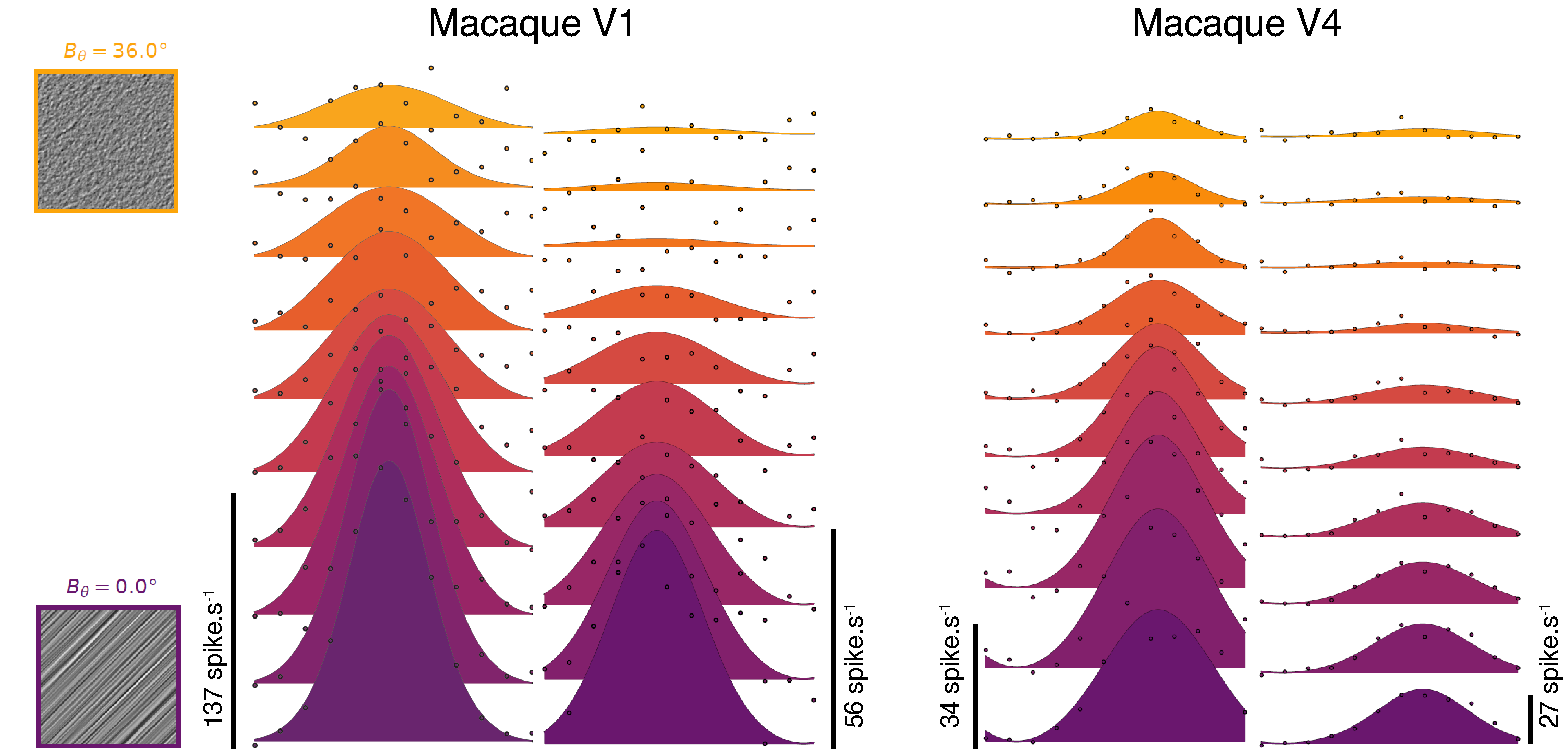
\includegraphics[width=1.\textwidth]{fig/chap4_utah_array.pdf}
\caption[Orientation variance modulations in macaques.]{Orientation variance modulations in macaque \gls{V1} and V4. Stimulation protocol is similar to the one presented in this chapter's article. These results will be further elaborated upon in chapter 5.}
\label{fig_chap4_utah_array} 
\end{figure} 

After having shown in this article a laminar (i.e., vertical) organization of variance computations, we turned to a new type of extracellular electrodes to extend those results. As interactions between neurons with different preferred orientation requires sampling of the orientation map, a horizontal probe is better suited to this task. As such, our results we replicated in awake macaque in Pieter Roelfsema's laboratory, using Utah arrays (Figure~\ref{fig_chap4_utah_array}), which are matrices of electrodes, consisting of $128$ recording sites in a 8x8 grid. Using the exact same type of stimulations (MotionClouds, rigit drift orthogonal to median orientation), we replicated similar neuronal behavior from anesthetized cats to awake primates, but also to extend our results into extrastriate areas, namely in V4. Interestingly, this not only holds for the single isolated neurons as shown in Figure~\ref{fig_chap4_utah_array}, but also for the response of neurons that are anatomically grouped. The specific advantages of this method of sampling are showcased in chapter 5, in which we infer functional connectivity directly into this data.




        %\input{tex_body/chap_pc}

        \chapter{Mapping Neural Interactions in V1: A Graph-Based Perspective}

\begin{flushright}
    \textit{''I won't be round this old town,  \\
            anymore for a long, long time, \\
            gonna hit the road and start looking for the end of that long white line''}\\
        Sturgill Simpson, Long White Line, 2014
\end{flushright}

\chaptertoc{}
\section{Introduction: Towards Mesoscale Recordings in V1}
Unlike the previous chapters in this manuscript, chapter 5 does not feature an already published or submitted article. This difference is due to the chapter focusing on a new set of experimental data, collected in Dr. Pieter Roelfsema's lab by Dr. Paolo Papale. These unique results stem from recordings in a single awake vigil macaque, which was initially implanted with Utah arrays for a different study. We were fortunate to have Drs. Roelfsema and Papale's support, allowing us to perform recordings linked to Motion Clouds in this primate model, building upon the discoveries highlighted in chapter 4.
However, it's important to note that standard practices for publishing require data from at least two primates. The decision to further collaborate and include a second primate in this study was contingent on the preliminary results obtained from the first primate. While this process is underway, it is expected that the resulting data will be available after the completion of this manuscript.

Therefore, chapter 5 will be structured similarly to an article, but will not include one. It will also be (very) short, compared to other chapters, as it mainly aims to reinforce significant concepts introduced earlier, although the current stage of the data is still too preliminary for a more extensive discussion.

Indeed, we will here build on an implicit concept of the manuscript's introduction: the notion that processing variance in low-level sensory cortices (i.e., \gls{V1}) relates to learning the structure of the variance in the environment. This proves advantageous for adaptive coding properties, and for redundancy elimination~\cite{barlow1961possible}. On a methodological point of view, extension from anesthetized cats to awake primates is not trivial (see also the conclusion of this manuscript). It eliminates the possible confounding factor of anesthesia, and enables comprehensive neurobiological sampling of recurrent activity with Utah arrays (Figure~\ref{fig_chap4_multielectrodes}).

This is a significant step forward from the approach in chapter 4, where we relied on interpolating through data from different sources and computational approximations to understand neural dynamics. In that sense, Utah arrays are advantageous by allowing for the sampling of multiple, distinct sites across the orientation map. However, Utah arrays present another challenge  due to their higher impedance (inverse of the resistance), meaning they effectively record from a larger area around their implantation site. This larger recording area makes it impractical to perform the precise spike sorting and manual curation, as done in chapter 4.

Instead, our approach will focus on \gls{MUA}. Recording \gls{MUA} is akin to recording the aggregated activity of nearby neurons, and has been shown to be a good proxy for single unit recordings in structured topological maps~\cite{bondy2018feedback, ni2018learning,lange2023weak} like \gls{V1}. Certain limitations apply: the temporal nature of the signal is less accurate, and if a given recording site happens to fall in the "pinwheel" of an orientation map (Figure~\ref{fig_chap2_vision_V1_ori_selec}), it is likely that competing interactions are going to be part of the signal recorded. Despite the different methodological constraints imposed by the use of Utah arrays, this chapter will extend on the notion that that computations of variance in neural signals are influenced by interactions among neurons, which are distributed, rather than concentrated, when variance increases. 



\section{Methods: Graphs of Neural Activity}
As described above, recordings were carried in a single awake, vigil macaque, with Utah arrays implanted in \gls{V1} and V4. Extrastriate data will not be part of the present manuscript, but do show similar modulation of orientation selectivity by orientation variance as \gls{V1} (as shown in Figure~\ref{fig_chap4_roelfsema}). This consistency across areas does suggest potential avenues for future research, discussed in the conclusion of the manuscript. 

To briefly detail the experimental setup, the framework was similar to that of chapter 4, modified with adaptation for primate recordings. Here, the macaque was engaged in a passive fixation task, which involved the presentation of Motion Clouds, shown for $300$ ms and interleaved with mean luminance screen for $150$ms. Median orientation $\theta$ was varied between $0;\pi$ in $12$ even steps, and orientation variance $B_\theta$ in $10$ steps between $\pi/30;\pi/3$. Other parameters were adapted from chapter 4 to match macaque \gls{V1} preference, namely a spatial frequency of $1.2$ cycles per degree, and a drifting speed of $3$ cycles per second~\cite{priebe2006tuning}. Stimuli were drifting in either direction, orthogonally to median orientation, and were averaged across direction. The macaque was headfixed, and observed a $1024$ by $768$ pixels screen from a distance of $47.5$cm. All stimuli were shown at least $40$ times. 

\begin{figure}[h!tbp]
\vspace{0.1cm}
\centering
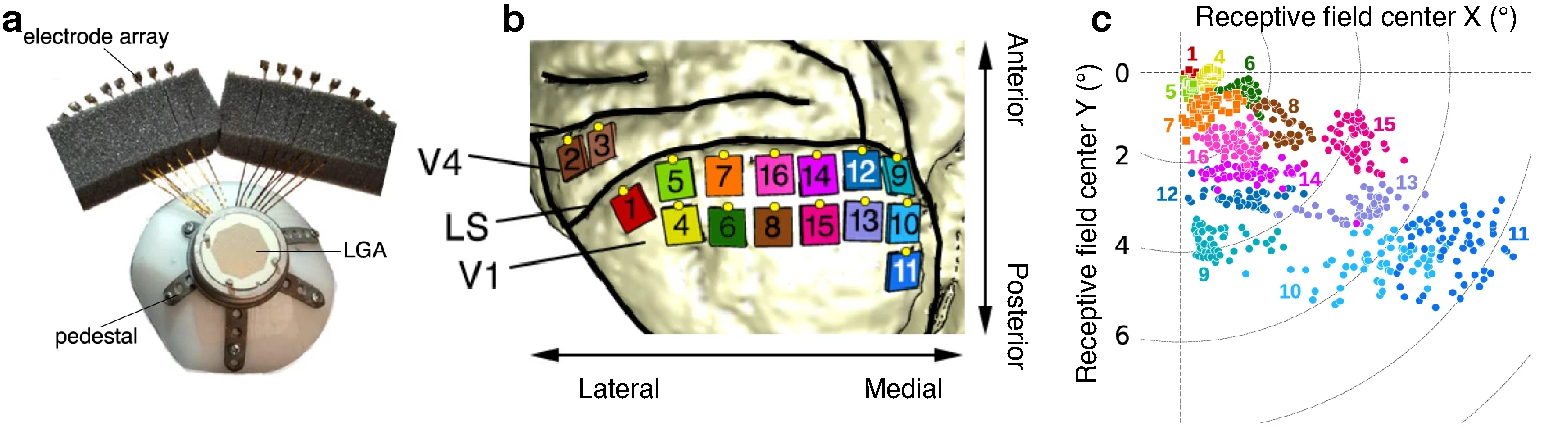
\includegraphics[width=1.\textwidth]{fig/chap5_1024chans.pdf}
\caption[Utah array recording in macaques.]{Typical setup of Utah array recording in macaque visual cortex, similar but not identical to the one used in the present chapter. (a) Example of a macaque implant, consisting of 1024 channels encased in a titanium cranial pedestal. (b) Typical layout of the arrays. Here, "only" 8 arrays, i.e. 512 channels, are implanted in \gls{V1}. (c) Typical eccentricity of the receptive field, as recorded here. Reproduced from~\cite{chen20221024}.}
\label{fig_chap5_1024chans} 
\end{figure} 

\gls{MUA} was recorded in $8$ Utah arrays, consisting of $8x8$ electrodes, hence totaling a number of $512$ electrode sites (Figure~\ref{fig_chap5_1024chans}). Given that the implantation of the chamber was done for another set of experiments, it was necessary to remove certain recording sites that were no longer yielding good signal~\cite{super2005chronic}. A signal-to-noise ratio was measured, based on evoked activity over resting ($300$ ms before evoked) baseline. This ratio was measured as the peak activity subtracted by mean resting activity, and normalized by the standard deviation of that resting activity~\cite{chen20221024}. Channels with a signal-to-noise ratio below $1$ were removed from further analysis, leaving $384$ electrodes. As in chapter 4, the circular variance served as a criterion for exclusion of untuned neurons. A threshold was set at $0.85$, removing untuned electrodes and leaving a final $188$ electrodes for analysis.

We thus aimed to analyze how information transfer between each of the remaining $188$ electrodes is affected by input variance. There are numerous ways ($237$, to be exact~\cite{cliff2023unifying}) to measure pairwise interactions between sets of time-based data, and each method comes with its unique benefits and limitations. Here, we decided to measure covariance, which is one of the simplest and most intuitive methods available, and represents how much two electrodes evolve together. This covariance matrix is similar to the matrix form of variance, but extended to multiple variables, as used in the matrix formulation of predictive processing (Equation~\ref{eq_pc_matrix}). Given a pair of electrodes $X$ and $Y$, the covariance at a single timepoint is: 
\begin{equation}
    \text{Cov}(X, Y) = \frac{\sum_{i=1}^{n} (X_i - \bar{X})(Y_i - \bar{Y})}{n-1}
\end{equation}
where  \( X_i \) and \( Y_i \) are the individual values of the signal in electrodes \( X \) and \( Y \) for a given trial $i$, \( \bar{X} \) and \( \bar{Y} \) are the mean values accross trials, and $n$ is the number of trials (here, $40$).

Not only is covariance straightforward to compute and interpret, but its matrix inverse is also useful, as it is the inverse variance matrix, which is the central focus of this thesis. When dealing with large datasets, like ours with $188$ variables (electrodes) but only $40$ observations (trials), directly inverting the covariance matrix can lead to instability due to the disproportionate ratio of variables to observations. To address this, we employ a technique known as a "shrinkage estimator". This method provides a more reliable estimation of the inverse covariance matrix, making it feasible for inversion. Here, we used the common Ledoit-Wolf estimator, which given a matrix $M$: 
\begin{equation}
    \hat{\Sigma}_{LW} = \alpha \cdot \text{F} + (1 - \alpha) \cdot \text{M}
\end{equation}
where \( \hat{\Sigma}_{LW} \) is the Ledoit-Wolf shrinked matrix, \( \alpha \) controls a shrinkage intensity, \( \text{F} \) is the target matrix (the identity matrix scaled by the average variance) and \( \text{M} \) is our sample covariance matrix. Here, $\alpha$ is automatically chosen to minimize the mean squared error of the reconstruction~\cite{ledoit2004well}~\footnote{A year before the publication of this article, these authors released a related article entitled "Honey, I Shrunk the Sample Covariance Matrix"~\cite{ledoit2003honey}. For some reason, the author of the present manuscript found this amusing enough to be note-worthy, and even considered at one point that it would make an excellent title for this chapter. This was eventually decided against, and regarded as a sign that it might be time to stop working on inverse variance-weighting and graduate.}.
The inverse variance matrix (or precision matrix), is thus $\hat{\Sigma}_{LW}^{-1}$.

A property of covariance matrices, and thus of inverse variance matrices, is their symmetry: the interaction between the electrode $X$ and $Y$ is the same as the interaction between electrode $Y$ and $X$. As a result, the interactions we observe between electrodes in this context are not directional; they only have varying degrees of intensity, or weight. While directional metrics might be useful for uncovering how information is transferred between neurons, potentially exposing interactions that are unique to specific orientations, this is being the scope of the current research.

We visualized these matrices as graphs, which are composed of nodes (representing electrodes) and edges (indicating covariance or inverse variance). This graphical representation makes it easier to comprehend the data, as the matrices in their raw form are not readily interpretable. Additionally, this approach offers a range of mathematical tools to analyze network variations. Here, the graphs are non-directional (because of the covariance or precision symmetry), cyclic (because they form closed interactions loop) and weighted (by the co-variance/inverse variance). 
To manage complexity and minimize noise, we binarized these graphs. This means we disregarded edges below a certain threshold, as a $188^2=35344$ edges-wide graph would be too unstable for analysis. We retained only those edges that ranked above the 75th percentile in weight distribution, a common practice in graph theory analyses~\cite{farahani2019application}, This narrowed the focus on the most significant interactions within the network, at the cost of full network representation.

The specific nature of the graphs we've created here limits the range of questions we can explore regarding their topology. To navigate this, we've selected six key metrics to analyze: clustering, centrality, assortativity, neighboring connectivity, small-worldness, and the Wiener Index~\cite{meunier2010modular,bullmore2012economy}. Mathematical details are provided hereafter, but are not necessary for the comprehension of the results. Rather, an intuitive description is provided with each equation, and a graphical representation is shown in Figure~\ref{fig_chap5_graph_metrics}.

\begin{figure}[h!tbp]
\vspace{0.1cm}
\centering
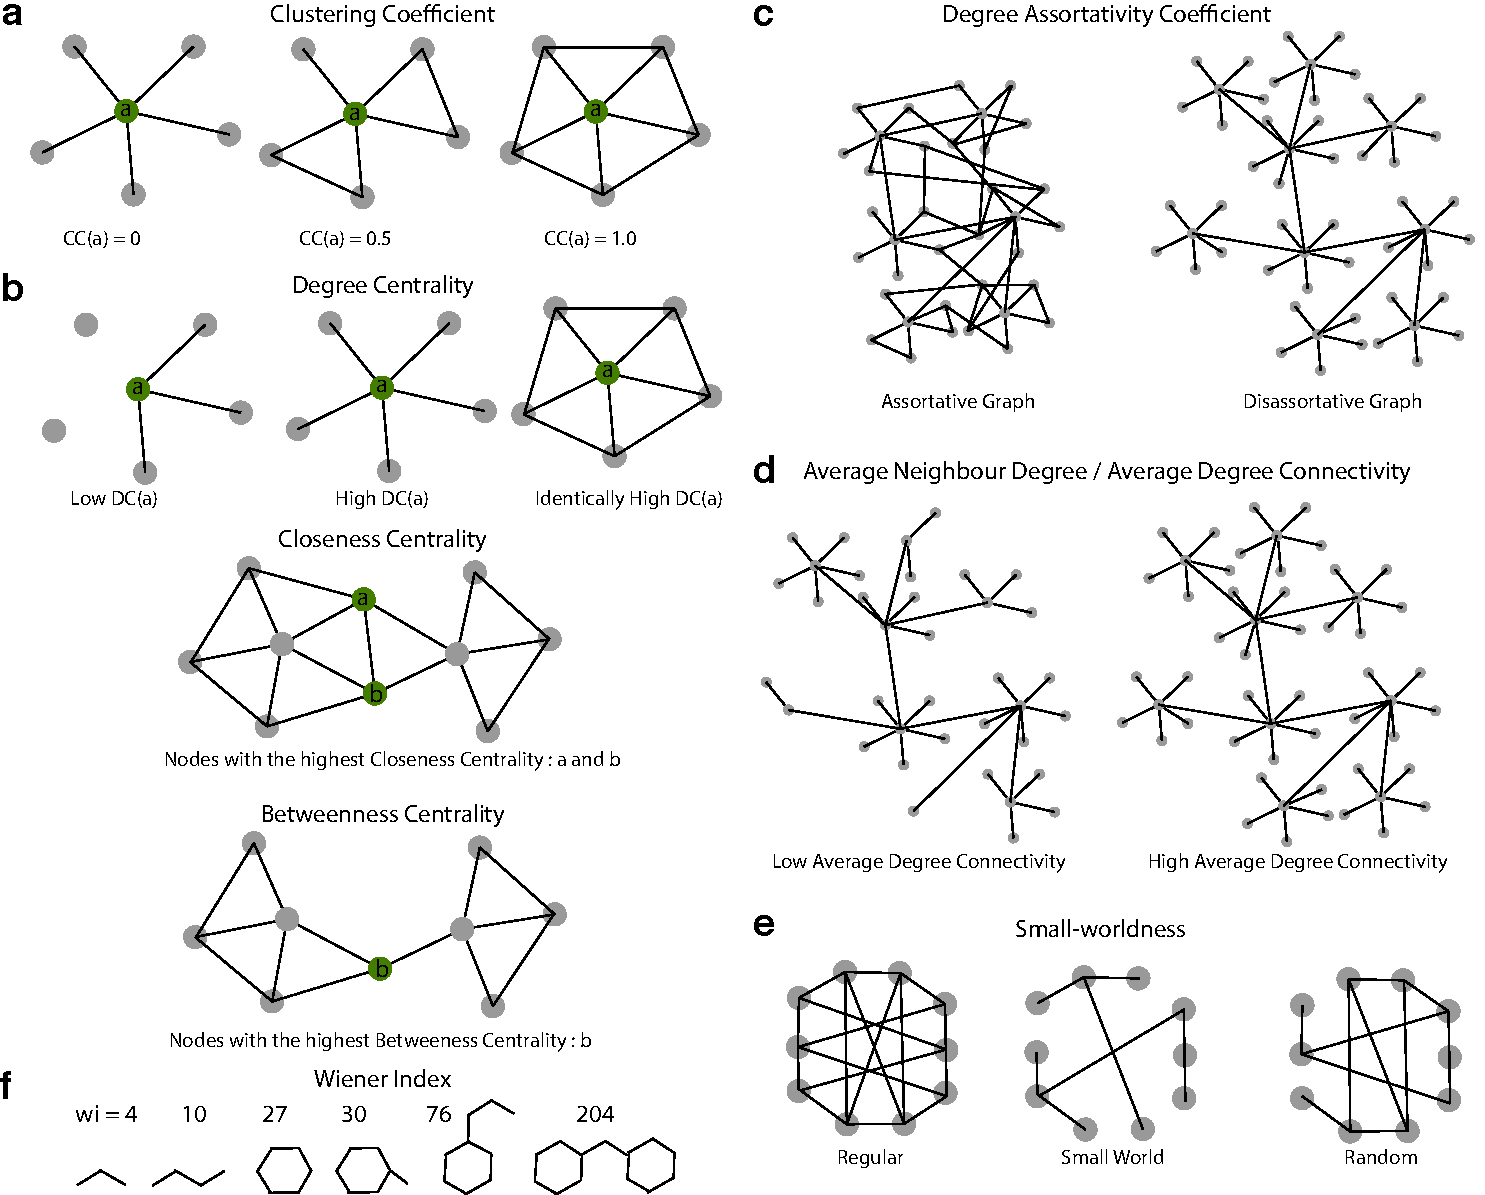
\includegraphics[width=1.\textwidth]{fig/chap5_graph_metrics.pdf}
\caption[Graph metrics.]{Graph metrics, presented in identical order as in the text below. (a) Clustering Coefficient, (b) Centrality metrics, (c) Degree Assortativity Coefficient, (d) Average Connectivity Metrics, (e) Small-worldness index, (f) wiener Index, represented onto common chemical compounds (delocalized electron cycles not shown).}
\label{fig_chap5_graph_metrics} 
\end{figure} 

The first metric used is the clustering coefficient, a measure of the degree to which nodes in a graph tend to cluster together. For example, in the context of a social graph, it helps understand the extent to which friends of a given person are also friends between each other. Here, it can be seen as a direct measure of the global interconnectedness of the neural network being recorded.
The equation for the clustering coefficient \( C_i \) of a node (electrode) \( i \) in a graph is:
\begin{equation}
    C_i = \frac{2T(i)}{k_i(k_i - 1)}
\end{equation}
where \( T(i) \) is the number of triangles through the node \( i \) (i.e., the number of connections that exist among the immediate neighbors of the node \( i \)) and \( k_i \) is the degree of node \( i \) (i.e., the number of edges connected to node \( i \)). \( C_i \) ranges from 0 to 1, with higher values meaning a greater degree of clustering. Here, all node-wise metrics were reported as a distribution of values across multiple input $\theta$, for each $B_\theta$.

A second metric, or rather, class of metric, is the measure of centrality. Multiple sub-metrics are available here, each with their own importance. We measured three, which are:
\begin{itemize}
    \item Degree Centrality: The simplest form of centrality. For a node in a graph, degree centrality is simply the count of how many connections (edges) it has. Nodes with higher degree of centrality are typically more influential or important in a network because they have more connections. Thus, the higher the overall Degree Centrality of a graph is, the more connected the graph is. Following the equation above, it is thus simply measured as $k_i$.
    
    \item Closeness Centrality: This centrality metric focuses on how close a node is to all other nodes in the network. It is defined as the reciprocal of the sum of the shortest path distances from a node to all other nodes in the network. A higher closeness centrality indicates that a node can spread information to all other nodes in the network through less synapses. It is often correlated with the metric above, but not necessarily (see Figure~\ref{fig_chap5_graph_metrics} for example). For a given node \( v \), the closeness centrality \( C_C(v) \) is:
    \begin{equation}
        C_C(v) = \frac{1}{\sum_{u \neq v} d(v, u)}
    \end{equation}
    where \( d(v, u) \) is the shortest-path distance between nodes \( v \) and \( u \), and the sum is taken over all nodes \( u \) in the graph except \( v \) itself.
    
    \item Betweenness Centrality: This centrality metric quantifies the number of times a node acts as a bridge along the shortest path between two other nodes. It captures the degree to which a node lies on paths between others, indicating its potential for control over information flow in the network. Nodes with higher betweenness centrality can have significant influence within a network, by virtue of their ability to gate message passing between other nodes. For a given node \( v \), the betweenness centrality \( C_B(v) \) is calculated as:
    \begin{equation}
        C_B(v) = \sum_{s \neq v \neq t} \frac{\sigma_{st}(v)}{\sigma_{st}}
    \end{equation}
    where \( \sigma_{st} \) is the total number of shortest paths from node \( s \) to node \( t \), \( \sigma_{st}(v) \) is the number of those paths that pass through \( v \). The sum is computed over all pairs of nodes \( s \) and \( t \) in the graph, where \( s \neq t \neq v \).
\end{itemize}

A third metric is the Degree Assortativity Coefficient. It measures the tendency of nodes to connect to other nodes which have similar degrees. In other terms, it reflects whether high-degree nodes (nodes with many connections) tend to be connected to other high-degree nodes, and similarly for low-degree nodes. The Degree Assortativity Coefficient \( r \) can be calculated using the Pearson correlation coefficient for degree-degree pairs across all edges in the network. The formula is as follows:
\begin{equation}
    r = \frac{\sum_{jk} jk (e_{jk} - q_j q_k)}{\sigma_q^2}
\end{equation}
where \( e_{jk} \) is the proportion of edges in the network that connect a node of degree \( j \) to a node of degree \( k \), \( q_j \) is the proportion of ends of edges that are attached to nodes of degree \( j \) (also known as the "normalized degree distribution") and \( \sigma_q^2 \) is the variance of the distribution \( q \). The assortativity coefficient \( r \) ranges from -1 to 1. A value of 1 indicates perfect assortative mixing patterns, 0 indicates non-assortative mixing, and -1 indicates perfect disassortative mixing. Understanding the degree assortativity of a network is essential in analyzing the robustness and the dynamics of information or disease spread within the network. Thus, if high-degree nodes tend to connect with low-degree nodes, the network exhibits negative degree assortativity, as shown here. 

Fourth are degree metrics, namely, the Average Neighbor Degree and the Average Degree Connectivity. 
The Average Neighbor Degree is a measure for each node in a network, that is the average degree of its neighboring nodes. This measure is useful for understanding the tendency of nodes to connect to others that are similarly well-connected or not; much like the Degree Assortativity Coefficient. For instance, in a network with high degree correlation (assortativity), high-degree nodes tend to be connected to other high-degree nodes. For a node \( v \) with degree \( k \), the Average Neighbor Degree \( \text{AND}(v) \) is given by:
\begin{equation}
    \text{AND}(v) = \frac{1}{k} \sum_{u \in N(v)} \deg(u) 
\end{equation}
where \( N(v) \) denotes the set of neighbors of \( v \), and \( \deg(u) \) is the degree of a neighbor \( u \). 
The Average Degree Connectivity, on the other hand, is a network wide metric that measures the average degree of the neighbors of nodes with a given degree. As such, it is often correlated with the $\text{AND}$. The Average Degree Connectivity for nodes of degree \( k \) in a network, denoted as \( \text{ADC}(k) \), is defined as:
\begin{equation}
    \text{ADC}(k) = \frac{1}{N_k} \sum_{v: \deg(v) = k} \text{AND}(v)
\end{equation}
where \( N_k \) is the number of nodes with degree \( k \) in the network. Their interpretation, similar to the Assortativity Coefficient, gives insight into whether the network is assortative or disassortative (Figure~\ref{fig_chap5_graph_metrics}).

A fifth metric is the degree of small-worldness, which quantifies a network in which clustering coefficient is high, while maintaining short average path length. In neural networks, this results from the balance between minimizing the resource cost and maximizing the flow of information among the network components. In brain-wide networks, the metabolic cost between neighboring neurons is much lower than that of distant neurons, and thus the brain behaves a small-world network~\cite{liao2017small} to increase efficiency, as described in the introduction of this manuscript~\cite{barlow1961possible}.
A direct measure of small-worldness compares the current graph with a random network~\cite{watts1998collective}. This measure of small-worldness quantifies the balance between local clustering and global reach in a network. Specifically, small-world networks have significantly higher clustering than random graphs but similar average path lengths. Thus, the small-worldness \( S \) of a network can be quantified as follows:
\begin{equation}
    S = \frac{C / C_{random}}{L / L_{random}}
\end{equation}
where \( C \) is the average clustering coefficient of the network, \( L \) is the average shortest path length of the network, \( C_{random} \) and \( L_{random} \) are the average clustering coefficient and average shortest path length, respectively, of an equivalent random graph. Typically, a network is considered to exhibit small-world properties if \( S > 1 \), indicating that it has higher clustering than a random graph while maintaining a comparable average shortest path length. 

Finally, a sixth metric is the Wiener Index, one of the oldest topological indices~\cite{diudea1998wiener} that is used primarily in chemical graph theory (see Figure~\ref{fig_chap5_graph_metrics}). It is a measure of the compactness of a network and is closely related to the small-worldness and efficiency of the network.
 The Wiener Index \( W \) of a network is defined as:
 \begin{equation}
     W = \sum_{\{i,j\} \subseteq G} d(i, j)
 \end{equation}
which is the sum of the shortest path lengths between all pairs of nodes in the graph. In this context, \( G \) is the set of nodes in the network, and \( d(i, j) \) represents the shortest path between nodes \( i \) and \( j \).



\section{Results: Modulations of Connectivity Patterns by Orientation Variance}
Before diving into graph metrics, let us first assess direct \gls{V1}-based metrics. Namely, we will first observe whether the variance-tuning curves shown in chapter 4 are also present in primate \gls{V1}. In this part of our study, the reliance on \gls{MUA}, rather than single-neuron activity,  means we lose the granularity of precise spike timing. There are however notable parallels in how both \gls{MUA} and single neuron activities in terms of orientation tuning~\cite{lange2023weak}. 

This holds true here, as the variance-tuning functions reveal similar patterns of activity modulation across neurons as shown in chapter 4. Despite the shift in scale from single neurons to \gls{V1}, we observe a comparable distribution of heterogeneous modulations in neuronal activity, as shown in Figure~\ref{fig_chap5_nkr}. This validates the consistency of our findings across different levels of neural activity and species. This, in turns, allows us to extrapolate (with caution) some similarities between the precise single-neuron mechanism of chapter 4 and the graph metrics of this chapter.

\begin{figure}[h!tbp]
\vspace{0.1cm}
\centering
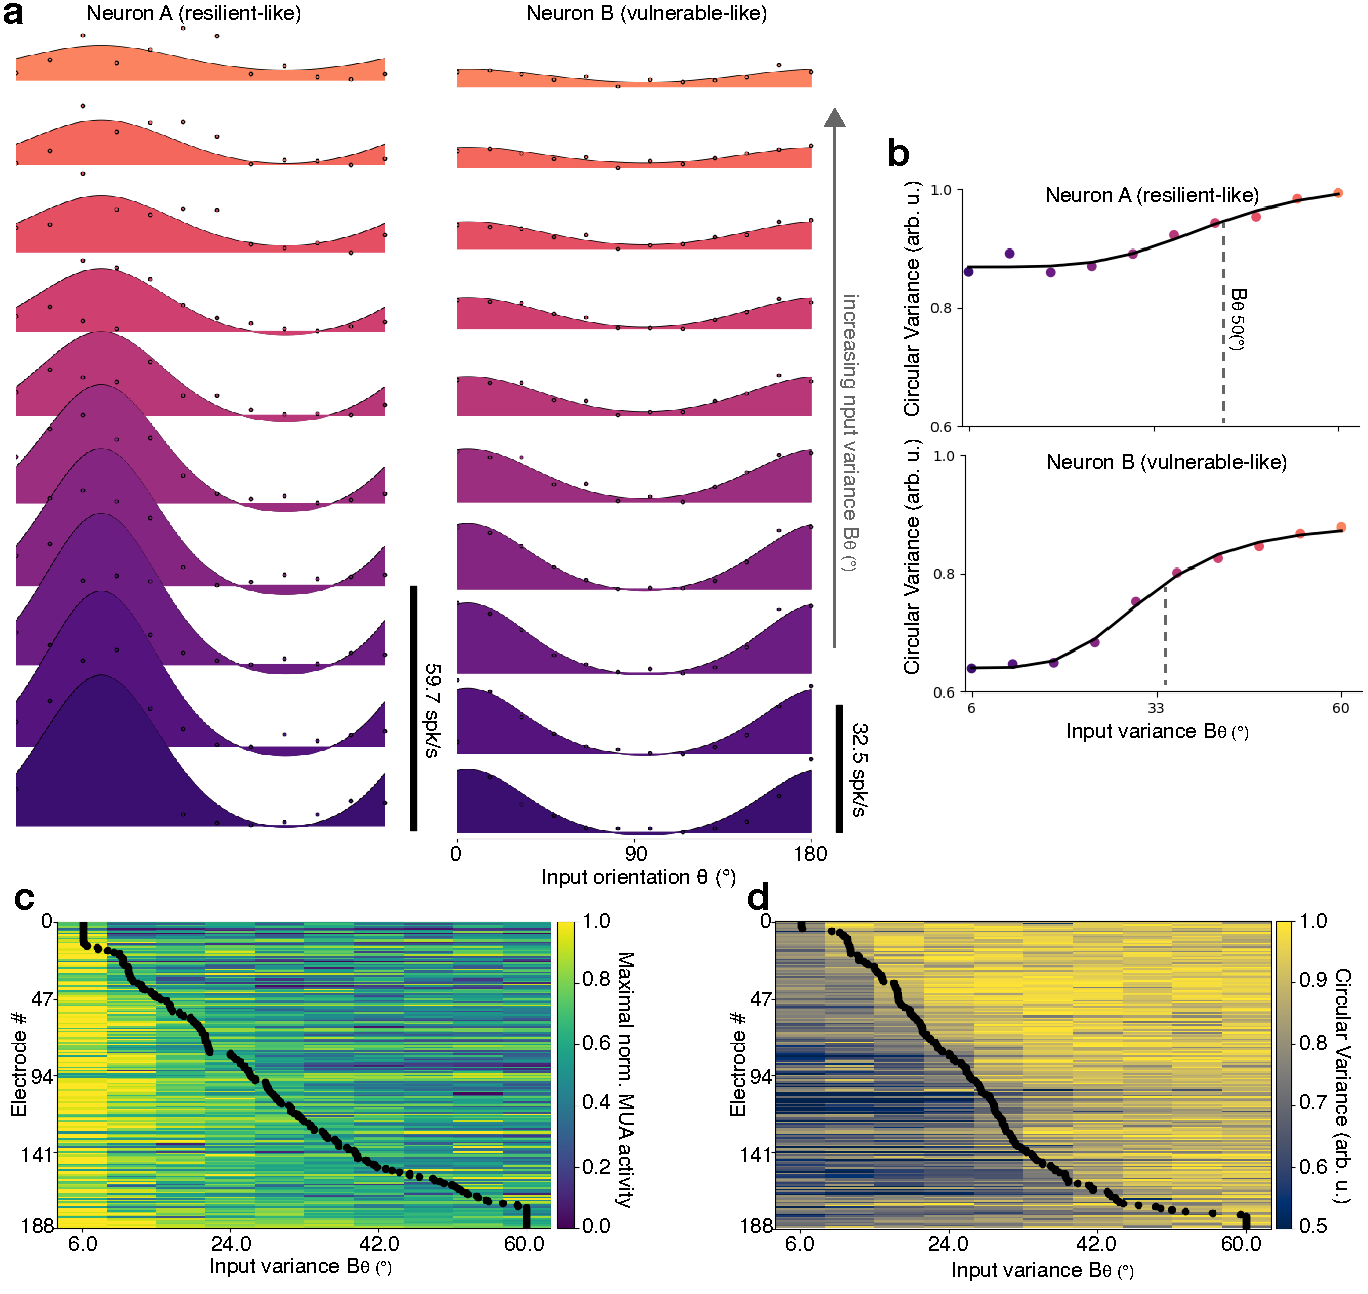
\includegraphics[width=1.\textwidth]{fig/chap5_nkr.pdf}
\caption[Variance tuning functions in primate V1.]{Variance tuning functions in primate \gls{V1}. (a) Modulation of tuning curve for two example \gls{MUA}, reminiscent of resilient/vulnerable neurons described in chapter 4. (b) Variance-tuning functions of these two examples \gls{MUA}, fitted with a Naka-Rushton function (black line). (c) Population map of variance-tuning functions, with dots representing $B_{\theta50}$, the changepoint of the function (see chapter 4). (d) Population map of variance-tuning functions, as with (c).}
\label{fig_chap5_nkr} 
\end{figure} 

While timing modulations are present (data not shown), in practice, these were on the order of tens of milliseconds in single neurons (i.e., about one $\tau$), and thus, it would be hard to extrapolate these in \gls{MUA} due to smoothing across multiple neurons. Given these constraints, our analysis at the single-electrode level is largely limited to tuning metrics. Hence, we turn our focus to mesoscale measurements, which offer a broader view of neural activity while still providing valuable insights. 
An example of such a mesoscale measurement is neural decoding, as we explored in chapter 4. Decoding would have been a particularly interesting approach in this context, especially since the activity is recorded in physical simultaneity, as opposed to virtually concatenated in chapter 4. Given similiarities in tuning, we might hypothesize that the decoding results in primate \gls{V1} would mirror those found in cat. This assumption is based on the consistent tuning characteristics observed across different animal models, suggesting a fundamental similarity in how \gls{V1} processes visual information.

However, here, we tried to branch away from simply reproducing chapter 4 results, and opted to investigate the interactions between neurons, as opposed to decoding an emergent neural code. As detailed in the methods section, to explore this, we utilized covariance matrices and their inverses, the inverse variance matrices, as our primary analytical tools.
For the $188$ electrodes, such matrices are shown in Figure~\ref{fig_chap5_matrices}. These represent the interactions between neurons, and characterize the variation of recurrent message passing between neurons. Here, there are measured for a single input $\theta$, which was chosen as the one with most \gls{MUA} tuned onto. We reasoned that this would be the orientation for which the representation would be the most accurate, but we will then average metrics across orientations in later sections.

\begin{figure}[h!tbp]
\vspace{0.1cm}
\centering
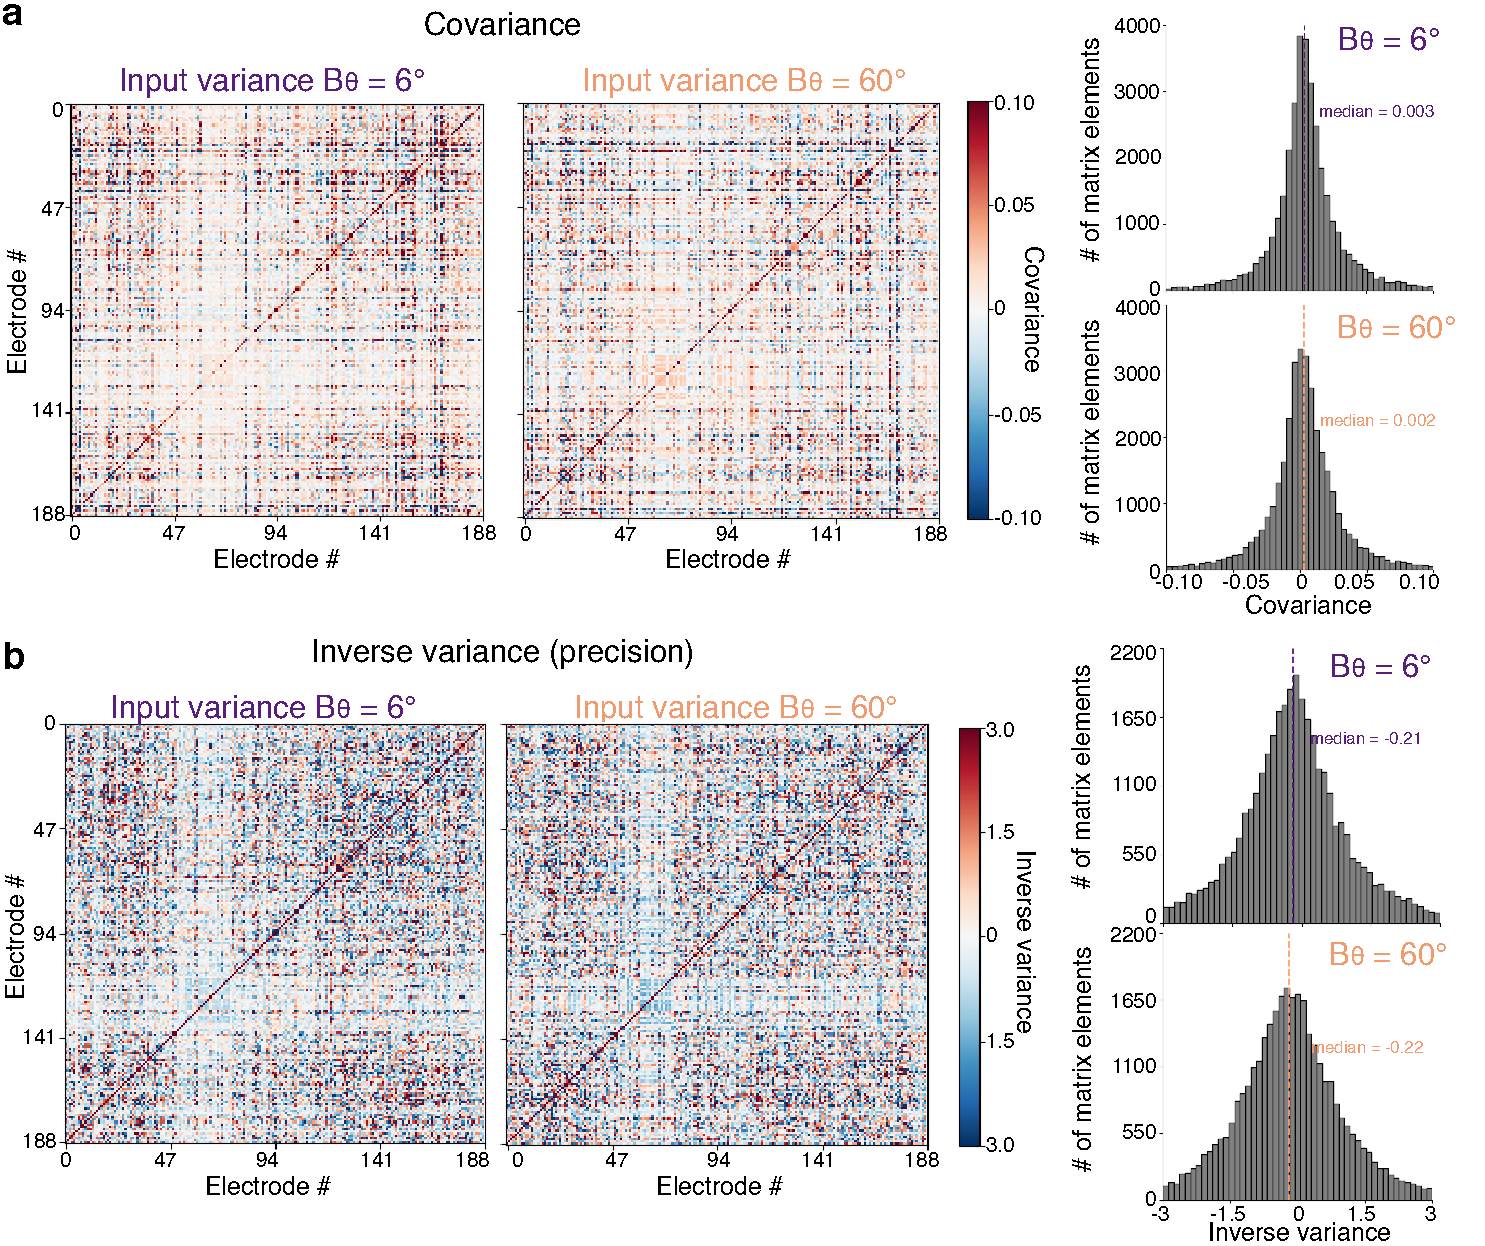
\includegraphics[width=1.\textwidth]{fig/chap5_matrices.pdf}
\caption[Covariance matrices in primate V1.]{Inverse variance-weighting in primate \gls{V1}. (a) Covariance matrices for lowest and highest variances, for a single orientation. The order of the elements, from $0$ to $188$, follows the preferred orientation at each electrode. Distribution of the covariances values with median value is shown in the right. (b) Same as (a), but for inverse variance (precision) matrices. }
\label{fig_chap5_matrices} 
\end{figure} 

Interpreting connectivity differences solely from the matrices can be challenging, and one often sees what they wish to be true. Even employing ratios or advanced metrics like the Laplacian or matrix-norm doesn't significantly enhance our understanding of these interactions. To mitigate this, we later broaden our approach to average across different orientations, aiming to capture a more comprehensive view of neuronal interactions across the visual spectrum. This expanded analysis is part of our ongoing effort to better understand the intricate web of connections and influences within neural networks.

Thus, it is better to embed these matrices into graphs, which offers better representations and better metrics. These graphs can be plotted onto a tuning ring, where each node's preferred orientation corresponds to a specific position on the circle. This is a neurobiological realization of the computational "ring" model we presented in chapter 4. By positioning neurons according to their orientation preferences, we create a visual map that reflects the inherent structure of neural preferences and interactions in the visual cortex. This is shown in Figure~\ref{fig_chap5_circ_graphs}, which shows a clear variation on the condition of interactions.

\begin{figure}[h!tbp]
\vspace{0.1cm}
\centering
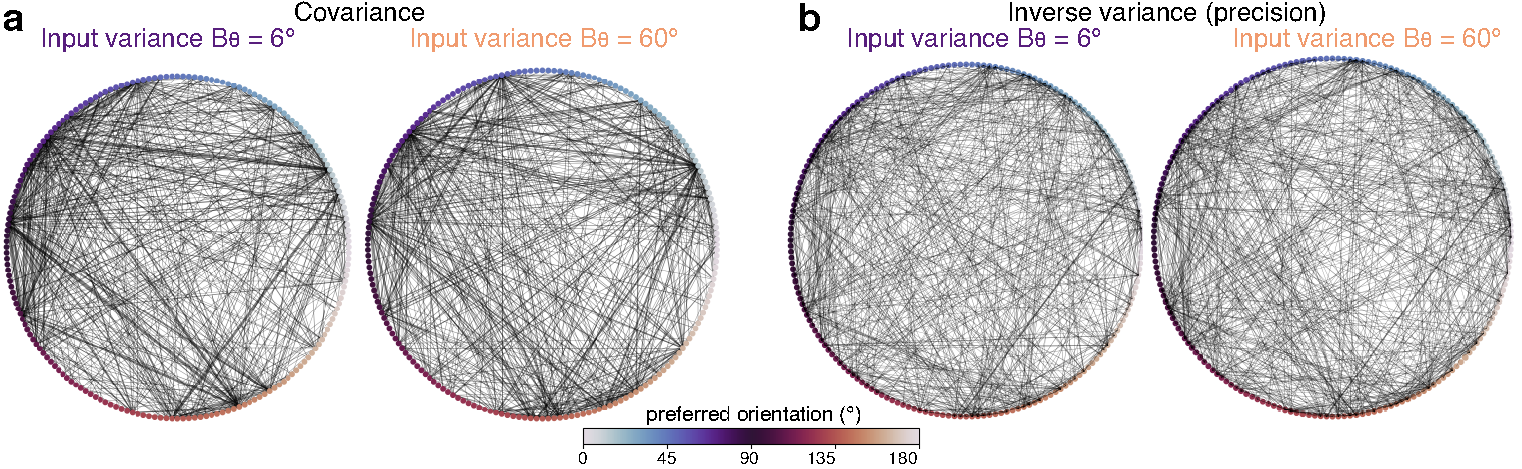
\includegraphics[width=1.\textwidth]{fig/chap5_circ_graphs.pdf}
\caption[Circular graphs of inverse variance.]{Circular graphs of inverse variance-weighting in primate \gls{V1}. (a) Graphs of covariance, with units sorted by their preferred orientations, for lowest and highest variances. (b) Same as (a), but for inverse variance.}
\label{fig_chap5_circ_graphs} 
\end{figure} 

This translates into an immediate, non-scientific conclusion: increasing the variability of input tends to complexify the graph's appearance. There is little to interpret with these representations, as the graph used here are fully connected (due to being based on covariance matrices).
How does this translate into pratical interactions? A more effective method for visualizing these graphs is through a force-directed algorithm, specifically the Fruchterman-Reingold force-directed algorithm, often referred to as a spring layout~\cite{fruchterman1991graph}. This attempts to maintain a certain distance between each node, essentially pushing them apart, but holding them together through their interactions. For instance, positive inverse variance-weighting draws the nodes closer, whereas negative weighting drives them even further apart. This represents the graph in a manner where all the connections (edges) are relatively equal in length and overlap as little as possible, creating a graph that is more straightforward to comprehend. This is shown in Figure~\ref{fig_chap5_force_graphs}.

\begin{figure}[h!tbp]
\vspace{0.1cm}
\centering
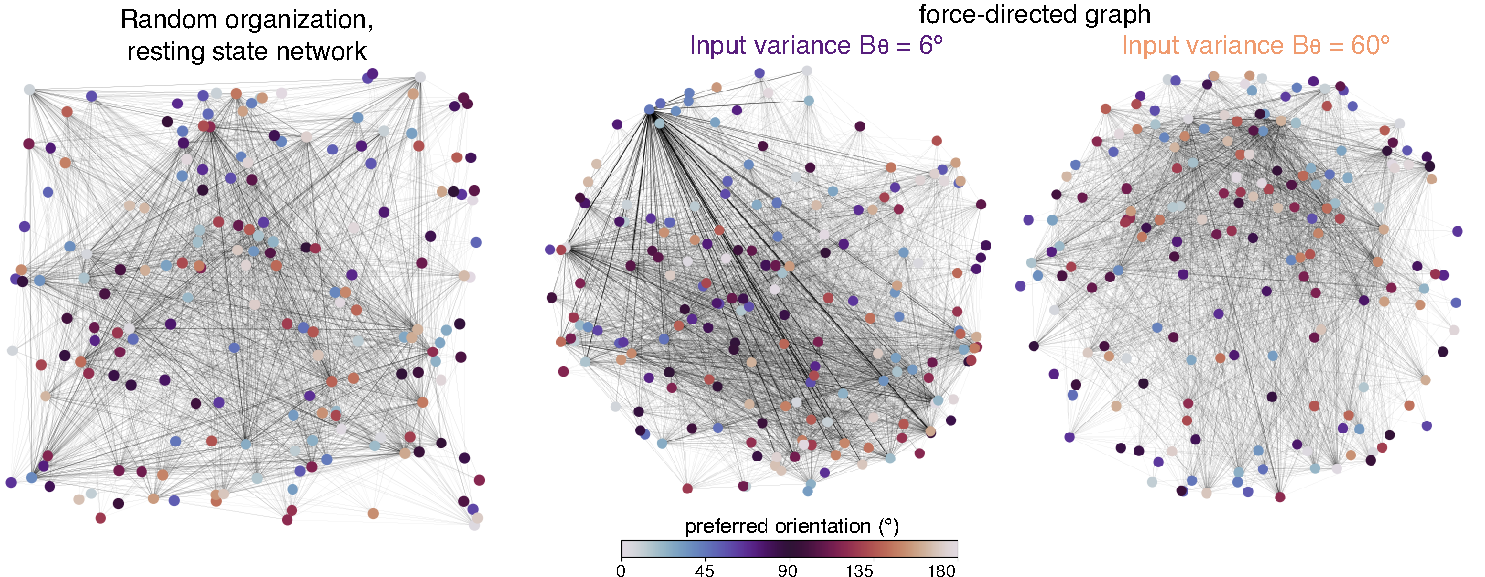
\includegraphics[width=1.\textwidth]{fig/chap5_force_graphs.pdf}
\caption[Force-directed graphs of inverse variance.]{Force-directed graphs of inverse variance-weighting in primate \gls{V1}, initialized from random positions (left), for lowest (middle) and highest variance (right).}
\label{fig_chap5_force_graphs} 
\end{figure} 

This is now steering us towards a clearer interpretation of the graph's dynamics. Through these representations, it becomes evident that with maximum input variance, the network's structure transitions from a dense, small-world configuration (concept introduced in Figure~\ref{fig_chap5_graph_metrics}) to a more dispersed, globally distributed network. This observation aligns with the concepts introduced in chapter 4, namely the idea that computations within the network become more iterative and distributed when dealing with high variance, in contrast to being more concentrated and feedforward-based for inputs with low variance. 

To properly quantify this phenomenon, we will now turn to the metrics that have been described in the methods section above (Figure~\ref{fig_chap5_quantification_graphs}). In the order in which they have shown in Figure~\ref{fig_chap5_graph_metrics}, these metrics paint a converging picture:
\begin{itemize}
    \item Clustering Coefficient increases as a function of input variance (Mann-Whitney U test between $B_\theta = 0$° and $60$° : $U=0.0, p<0.0001$. Linear regression : $y = 0.004x+0.68$, $p = 0.01$).
    Intuitively, this means that the neural activity in \gls{V1} is becoming more interconnected, as opposed to separated into uncorrelated sub-networks. This implies a shift from isolated processing to more integrated, recurrent neural activity, where neurons are not just operating independently, but are increasingly interlinked.
    
    \item Degree Centrality ($U=1968.5, p<0.0001$. lin. reg. : $y = 0.006x+0.65$, $p = 0.005$) and Closeness Centrality ($U=1994.0, p<0.0001$. lin. reg. : $y = 0.003x+0.74$, $p = 0.006$) increase as a function of input variance.
    This gives a similar interpretation as with the Clustering Coefficient, that of a network whose units are processing information in a more distributed fashion. Betweenness Centrality, however, is decreasing with input variance, ($U=19555.0, p<0.0001$. lin. reg. : $y = -0.00003x+0.001$, $p = 0.005$), suggesting that fewer nodes are acting as critical bridges within the network. This could mean that the network is becoming less reliant on given neural pathways, and distributes its processing load more evenly across the network.
    
    \item Degree Assortativity Coefficient is negative for all input variance, but still increases with input variance (lin. reg. : $y = -0.005x-0.05$, $p = 0.0002$).
    This means that a dissasortative neural network is progressively reorganizing into a less-tightly organized assortative neural network. However, as this coefficient absolute value's does increase with variance, it indicates a shift towards a network where nodes are more likely to connect with similar nodes. This transition suggests a move from a more hierarchical or specialized network to a more homogenized one.
    
    \item Average Neighbour Degree is increasing with input variance ($U=0.0, p<0.0001$. lin. reg. : $y = 1.05x+124$, $p = 0.006$). This implies that that neurons are not only increasing their connections but are also tending to connect with other neurons that are similarly highly connected, hinting at a more uniformly interconnected network, where all neurons are part of equally significant ensembles of interactions.
    
    \item Small-worldness is decreasing with variance (lin. reg. : $y = -0.004x+1.06$, $p = 0.001$). This marks a departure from the dominant default-mode of connectivity in neural networks~\cite{meunier2010modular}, and as with Average Neighbour and Average Degree Connectivity, \gls{V1} is becoming less tightly organized and distributed.
    
    \item Wiener Index is decreasing with variance (lin. reg. : $y = -119x+23820.5$, $p = 0.004$). A decrease in this index is intriguing, as it suggests that the overall path lengths within the network are reducing. This could mean that despite the increase in distributed processing, the network is somehow becoming more efficient in terms of signal transmission distances, which could be due to the reorganization of connections in the network. One implication of this is that the seeming disorganization of the network is not so much a disorganization as it is a planned reorganization, into an equally efficient but topologically different neural network.
\end{itemize}
Overall, these findings are very exciting, as they all converge towards a similar observation: with increased input variance, \gls{V1} is actively being reorganized from a tightly segregated topology into a delocalized, recurrent processing neural network. How these metrics evolve through time could also align with the idea of dynamical processing of orientation variance, as exposed in chapter 4, and form a promising avenue of research.

\begin{figure}[h!tbp]
\vspace{0.1cm}
\centering
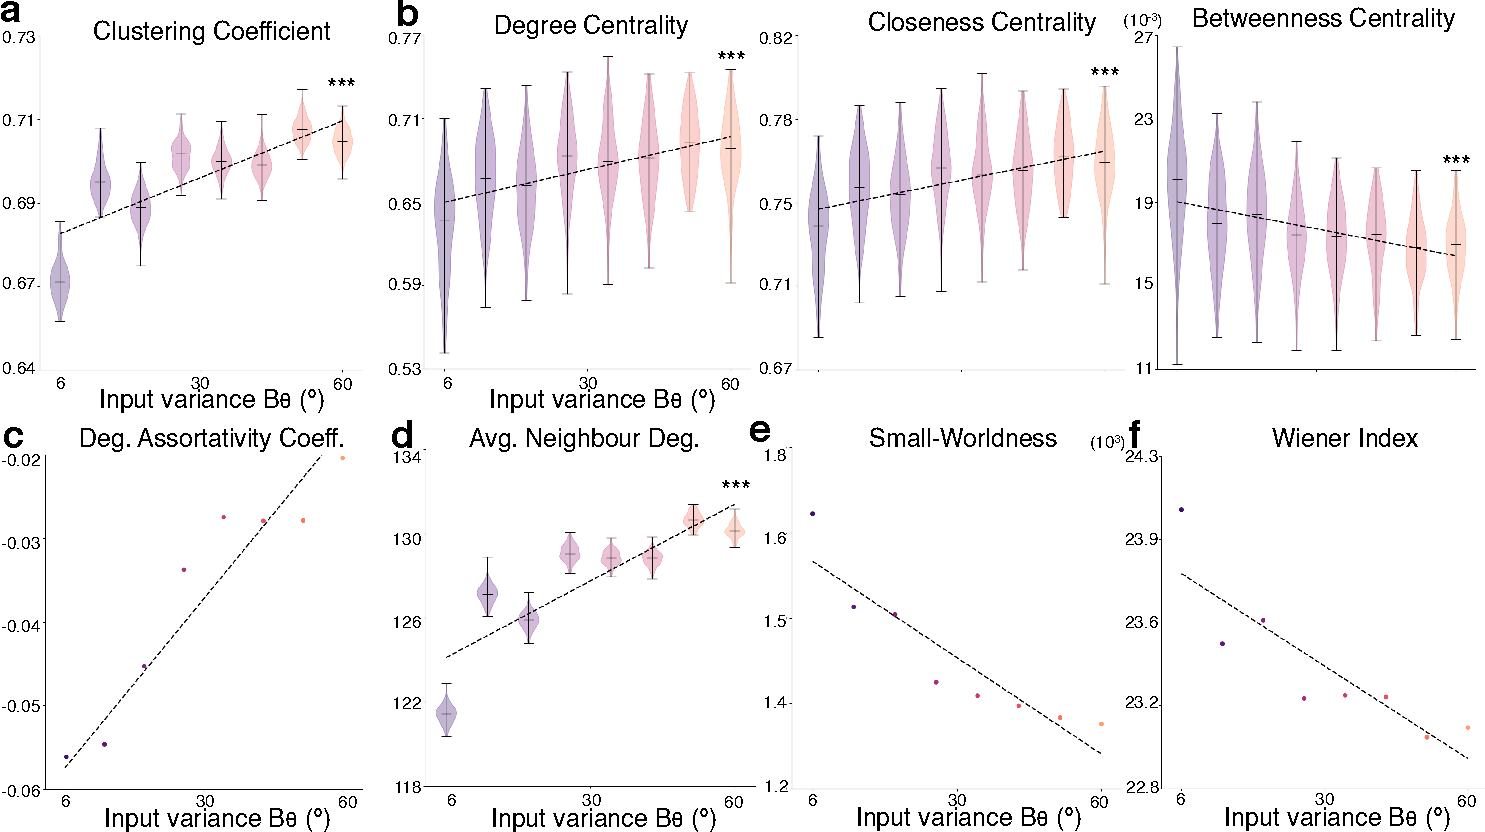
\includegraphics[width=1.\textwidth]{fig/chap5_quantification_graphs.pdf}
\caption[Quantification of graphs.]{Quantification of graphs. (a) Clustering Coefficient, showed as a violinplot with 5th, 95th quartiles and median values. Linear regression is shown as a dashed black line. Significance of the difference between $B_\theta=0$° and $60$° is indicated above the last boxplot (Mann-Whitney U test, $***;p<0.001$, $**;p<0.01$). (b) Centrality metrics. (c) Degree Assortativity Coefficent. (d) Average Neighbour Degree. (e) Small-Worldness. (f) Wiener Index.}
\label{fig_chap5_quantification_graphs} 
\end{figure} 

%These findings also extend the narrative established in chapter 4, aligning with an idea of dynamical processing of orientation variance observed in \gls{V1}.  Just as chapter 4 demonstrated that increased input variance necessitated extended processing time in \gls{V1}, the metrics here observed also show a temporal component. This suggests that the shift towards a decentralized network configuration is not a static alteration, but a dynamic property of the neural network, which could have been observed through the decoding process in chapter 4. TODO MORE HERE

%\begin{figure}[h!tbp]
%\vspace{0.1cm}
%\centering
%\includegraphics[width=1.\textwidth]{fig/chap5_dynamic_graphs.pdf}
%\caption[Dynamic modulation of graph through time.]{Dynamic modulation of graph through time. (a) }
%\label{fig_chap5_dynamic_graphs} 
%\end{figure} 



\section{Conclusion: A Predictive Coding Perspective}
Graph-based approaches to neuroscience often describes the brain as a small-world network~\cite{liao2017small}, which is a general principle of any system that balances efficiency and minimization of operating cost~\cite{sterling2015principles}. In the context of our manuscript, this means a series of networks that function in tandem, and are coordinated by broader neural interactions. Although the leap is theoretical, these can also be likened to a 'canonical microcircuit' model, where the brain processes sensory information (like orientation) and puts collaboration between adjacent circuits into play to form a comprehensive and integrated model of the environment.

Our research, particularly in Chapter 4, delved into the functional organization within a single cortical area, highlighting how single neurons and populations adapts to different variance in sensory input. We theorized an increase in recurrent neural activity in response to higher input variances.  Here, in awake vigil macaques, we show that is experimentally the case, using a graph theory approach that shows decentralization of the neural network as a function of the sensory input's variance. This aligns with our initial theory that the brain's segregated and linear processes evolve into more interconnected, decentralized operations involving multiple neurons, when faced with complex stimulus. This also implies that experiments based on stimulating \gls{V1} with drifting gratings are missing a crucial key component of the brain, that is, its network capacity to re-organize in face of sensory variance to adjust to an uncertain environment. 

The implications of these findings for predictive coding are significant. Let us now focus on the notion of variance, rather than inverse variance, as this will make more intuitive sense based on a Motion Clouds definition. If input variance increases in the visual input, patterns of activity across multiple orientation-tuned units in \gls{V1} also increase in variance (as also shown in chapter 4). This decentralization of the message passing between neuron implies that the distribution of neural activity, in orientation space, is a function of the distribution of input orientation.
As posited by predictive coding, lower-level (inverse) variance distributions in sensory areas are essential for learning the statistical variance in the environment. Essentially, the brain uses these lower-level distributions to fine-tune its predictions about the inherent variance in both the environment, but also in the sensors used to sample said environment. 

To validate this notion, one could imagine showing repeated high variance input to a macaque, and see how these response changes from a \gls{V1} that is used to process heterogeneous variance. One could then expect systematically broader patterns of activity in \gls{V1}.  Another way to explore these limits is to implement them into a predictive coding model, and see how this model behaves in the face of changing input variance. With the theoretical and mathematical framework already in place in the thesis' introduction, it would be rather straightforward to develop a neural network that implements predictive processing. This network could then be tasked with a simple machine learning classification task, for instance, solving the Modified National Institute of Standards and Technology database, a list of handwritten digits between 0 and 9. This task is trivial, and often the first one to be done on a newly developed neural network. Following this tradition, one could embed these digits into Motion Clouds, thereby manipulating the orientation distributions of these inputs and see whether similarities in the learned inverse variance matrix follow those observed in macaque \gls{V1}.

%As a reminder from $100$ pages ago, the general matrix form equation (i.e., Equation~\ref{eq_pc_matrix}) of predictive coding is:
%\begin{equation}
%    \begin{aligned}
%        \dot{\bar{\varepsilon}}_p &= \bar{\phi} - \bar{v}_p - \mathbf{\Sigma_p}\bar{\varepsilon}_p \\
%        \dot{\bar{\varepsilon}}_u &= \bar{u} - g(\bar{\phi}) - \mathbf{\Sigma_u}\bar{\varepsilon}_u \\
%        \frac{\delta F}{\delta \bar{v_p}} &= \bar{\epsilon}_p \\
%        \frac{\delta F}{\delta \boldsymbol{\Sigma_p}} &= \frac{1}{2}(\bar{\epsilon}_p\bar{\epsilon}_p^T - \boldsymbol{\Sigma_p^{-1}}) \\
%        \frac{\delta F}{\delta \boldsymbol{\Sigma_u}} &= \frac{1}{2}(\bar{\epsilon}_u\bar{\epsilon}_u^T - \boldsymbol{\Sigma_u^{-1}})
%    \end{aligned}
%\end{equation}
%Using Python and PyTorch, a code implementation of these equations is rather straightforward, and can be easily turned into a classification neural network (for details, see also~\cite{millidge2020relaxing}). This network can then be tasked with a simple machine learning classification task, for instance, solving the Modified National Institute of Standards and Technology database, a list of handwritten digits between 0 and 9. This task is trivial, and often the first one to be done on a newly developed neural network. Following this tradition, we will here embed these digits into Motion Clouds, thereby manipulating the orientation distributions of these inputs (Figure~\ref{fig_chap5_mnist}).

%\begin{figure}[h!tbp]
%\vspace{0.1cm}
%\centering
%\includegraphics[width=1.\textwidth]{fig/chap5_mnist.pdf}
%\caption[Classification of images with a predictive neural network.]{Classification of images with a predictive neural network. (a) %MNIST with hog below (b) Structure of the neural network. }
%\label{fig_chap5_mnist} 
%\end{figure} 

%Unsurprisingly, the network is able to achieve high accuracy on this classification task. One interesting result, however, is that increased input variance also increases the time to maximum accuracy, and even more so if the learning of inverse variance is disabled (i.e., set to identity matrices). This implies that learning the variance actually helps the neural network perform the classification task. As such, it is interesting to compare these inverse variance matrices, as we did in macaque \gls{V1}, and observe whether differences are taking place.

%\begin{figure}[h!tbp]
%\vspace{0.1cm}
%\centering
%\includegraphics[width=1.\textwidth]{fig/chap5_mnist_matrices.pdf}
%\caption[Inverse variance matrices of a predictive neural network.]{Inverse variance matrices of a predictive neural network. (a) }
%\label{fig_chap5_mnist_matrices} 
%\end{figure} 

% Indeed, as shown in Figure~\ref{fig_chap5_mnist_matrices}, there are striking similarity between these computational matrices and the data extracted from \gls{V1} recordings. Given that the neural network had to explicitely learn the variance of the input, this could indeed suggest that the dynamical restructuring of \gls{V1} are indeed related to learning the sensory variance of the world.

        \chapter{Beyond V1: Variance and Thalamo-Cortical Loops}

\begin{flushright}
    \textit{''Welcome back my friends \\
    to the show that never ends. \\
    We’re so glad you could attend, \\
    Come inside! Come inside!''}\\
    Emerson, Lake and Palmer, Karn Evil 9, 1973
\end{flushright}

\chaptertoc{}

\section{Introduction: The Functional Anatomy of the Pulvinar}
After having had the pleasure of immersing ourselves in more than a hundred of pages of \gls{V1}-centric research, it now seems only natural to take a break away from the striate cortex. As alluded to in the thesis's introduction, \gls{V1} takes part in parallel computations distributed both in extrastriate regions and in subcortical nuclei. These interactions are crucial for inverse variance processing, and now call for our attention for a proper description of a "multiscale" computational system. One particularly intriguing facet of these interactions is the role that the pulvinar nucleus plays. This thalamic nucleus operates as a sophisticated "routing" system, modulating the information flow between \gls{V1} and extrastriate regions~\cite{casanova2004functions}. Given the interest we took in the modulation of integration between multiple cortical regions by the inverse variance, the presence of a thalamic nucleus interconnected with this entire network is undeniably a brain region worthy of deeper exploration. 

Before detailing more the involvement of pulvinar in predictive coding, we shall briefly introduce its anatomy and functions. The first article of this chapter consists of a review of the role of pulvinar in this domain, aiming to introduce similar notions, and hence it would be redundant to go into too many details here. It should be noted that, in the context of this thesis, some theories suggest that the pulvinar might be the primary locus of inverse variance weighting in the brain~\cite{kanai2015cerebral}, while others suggest it only plays a part in this role~\cite{millidge2021predictive}.

Anatomically, the pulvinar lies over the dorsolateral posterior thalamus, running alongside the edge of the \gls{LGN}. In primates and in cats, the pulvinar is the largest thalamic nucleus, having increased in size throughout mammalian evolution with the visual cortex~\cite{hutchins1989retinotopic}. Given its size, the pulvinar can be further subdivided in six sub-regions in primates (human included) or three main regions in the cat~\cite{arcaro2015anatomical}, which, out of scope, will be here simplified as a single conceptual entity in this introduction (but see the first article for further details). The pulvinar establishes extensive reciprocal connections with all visual cortical areas~\cite{jones2012thalamus}, often being conceptualized as the "seventh cortical layer"~\cite{shipp2003functional}. In a striking difference with the \gls{LGN}, which receives its main visual inputs from the retina, the pulvinar receives its visual inputs principally from the layers 5 and 6 of the visual cortex. This is reflected in the response characteristics of its neurons, which remarkably resemble those found in the visual cortex in terms of feature selectivity~\cite{merabet1998motion}, but also in their implementation of selective attention~\cite{werner2004visual,villeneuve2012pattern}. This allows pulvinar neurons to effectively suppress responses to visual distractors~\cite{robinson1992pulvinar} by integrating the visual signals from multiple cortical areas and outputting modulatory signals to layers IV and I of the visual cortex. Overall, the pulvinar’s connectivity gives it an integrate-and-modulate role within the visual hierarchy. This description is especially relevant when considering the visual system as a hierarchical generative Bayesian model within the predictive coding framework (Equation~\ref{eq_pc_matrix}).

As put forward by Kanai et al.~\cite{kanai2015cerebral}, the pulvinar’s engagement in attentional regulation and its output connectivity to superficial cortical layers is an ideal match for a role in inverse variance modulation of the visual hierarchy, which also fits the long timescales of multi-areas integrations. Experimental results have shown that inactivation of the pulvinar drastically suppresses responses of superficial \gls{V1} neurons to sensory inputs, while excitation increases the responsiveness of neighbouring superficial units with overlapping receptive fields~\cite{purushothaman2012gating}, which is similar to a gain-control mechanism that implements inverse variance-weighted modulation of the cortex by the pulvinar. Whilst it is the biggest thalamic nucleus in primates, the pulvinar is nonetheless an order of magnitude smaller than the entire visual cortex. As estimating inverse variance requires computting the co-variance between the all $N$ prediction or prediction errors units, this is an $N^2$ computation~\cite{millidge2021predictive}. Given the cost of such computation, it seems more likely that the pulvinar computes an approximation of the inverse variance matrix, and then modulates parts of the superficial layers independently. In parallel, these units will then use their local horizontal connectivity to further integrate and refine the computation of the local variance~\cite{kanai2015cerebral, bastos2012canonical}, as proposed in chapter 4~\cite{ladret2023cortical}. Evolutionarily, this hypothesis is very interesting, as some species, such as birds, have much lower homologous "cortical" (i.e. pallium) neuron count, and seem to lack a functional equivalent of the pulvinar. In a thesis committee discussion with Dr. Paul Cisek, we hypothesized that as the number of neurons grow exponentially throughout evolution, computing variance through recurrence alone (as proposed in chapter 4), becomes either prohibitively slow or computationally expensive. This thus requires a dedicated central part of the neural network to perform a dynamical approximation of the inverse variance matrix, which would hence be the role assigned to the pulvinar.

\begin{figure}[h!tbp]
\vspace{0.1cm}
\centering
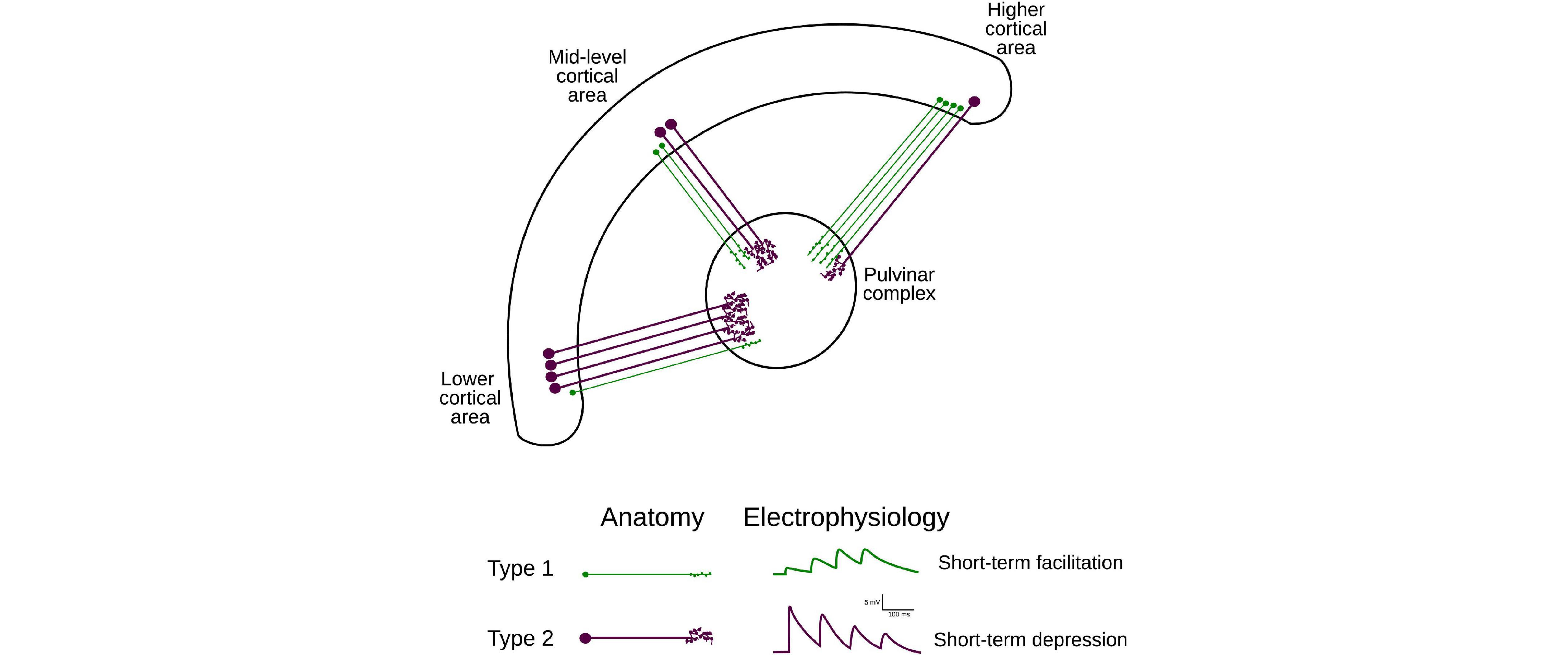
\includegraphics[width=1.\textwidth]{fig/chap7_gain_control.pdf}
\caption[Anatomical substrates of pulvinar gain control.]{Anatomical substrates of pulvinar gain control, from~\cite{cortes2021corticothalamic}. Note that the ratio of Type 1 over Type 2 synapses changes as a function of the visual hierarchy.}
\label{fig_chap7_gain_control}
\end{figure}

Overall, this depicts a dynamical gain control role for the pulvinar, much like the gain control role we proposed in chapter 4. How is such dynamical gain control in the visual cortical areas implemented ? Guillery and Sherman~\cite{guillery2002thalamus} characterized synapses associated to thalamic first-order relays, which transfer information about the world to primary cortical areas (in vision, the \gls{LGN}). Two types of inputs, modulators and drivers (type 1 and type 2 projections, respectively), have been identified on the basis of their axon terminals’ morphology and their electrophysiological characteristics~\cite{sherman1998actions}. Drivers and modulators can also be defined by other attributes, such as the input-output transfer of the neuronal response profile. Modulators effects are distinguished as either multiplicative or divisive effects (nonlinear gain control), while drivers act by either additive or subtractive changes (linear gain control)~\cite{abbott2005drivers, silver2010neuronal}. In \gls{V1}, it is generally accepted that pulvinar receives type II projections (confirmed driver signals) from layer 5 neurons and sends back anatomically defined type I projections (modulatory) to layer 1. In the case of higher-order cortical areas, the assumption is that pulvinar receives type I projections from layer 6 neurons (suspected modulators) and projects to layer 4 (suspected drivers) (Figure~\ref{fig_chap7_gain_control}. In the context of predictive coding, this functional distinction between drivers and modulators is crucial, as drivers are associated with predictions and modulators with precision. Precision may coordinate and broadcast more globally visual information and its regulation may be equivalent to selective attention~\cite{creutzfeldt1988extrageniculo}, which can be implemented by modulator connectivity from the pulvinar. This notion of driver and modulators will be discussed further in the first article of this chapter, which reviews additional functional evidences, but also in the second article, which models the heterogeneity of these two types cortico-thalamic pulvinar connections and their role on the propagation of prediction-related alpha oscillations. 

\section{Review: "The Pulvinar as a Hub of Visual Processing and Cortical Integration"}
This review for \textit{Trends in Neuroscience} aims to provide an overview of the hypothesized roles of the pulvinar. Given the extensive connectivity, one can find what they would like to find in this nucleus, and thus we aim to review the recent evidences for pulvinar in terms of attention, feature binding, predictive coding, and global workspace theory. 

Full citation is as follows: \fullcite{cortes2023pulvinar}

As this is a review rather than a research article, we direct the reader to Appendix B. There, they will find a comprehensive overview of the response properties of the pulvinar and their interpretation under predictive processing.



\section{Methods: Oscillations and Predictions}
As we discussed in the introduction and in the review, the pulvinar is involved in performing a gain control modulation onto \gls{V1}~\cite{purushothaman2012gating}. This can be conceptualized as a (predictive) gating mechanism, that can control the propagation of message passing from \gls{V1}. In the case of an overly high variance input, the pulvinar can thus "explain away" the activity of \gls{V1}, preventing an erroneous update of the internal brain models. But, in the opposite case, what is the influence of \gls{V1} on the pulvinar ? If, according to our article in chapter 4, \gls{V1} can compute the inverse variance of visual inputs, then it should be able to send that information in some form to the global regulator of the message passing to other cortical areas. Furthermore, if there is such a thing as this global regulator of inverse variance-weighting implemented the pulvinar~\cite{kanai2015cerebral}, then it is crucial to look at how \gls{V1} it interacts with the pulvinar, in that directed fashion. 

To understand the nature of this communication, we must first understand the nature of the message being sent. Disentangling sensory predictions from prediction errors is already arduous enough in \gls{V1} and we must turn our attention to another method to study inter-area communications. For that, it is better to study the propagation of activity from the cortex to the pulvinar in terms of frequency. This relies on the idea that, in predictive coding, one posits the existence of a single prediction error unit (not necessarily a neuron) for every prediction unit. As these units must be connected only to one another, and in the form of a negative feedback loop (see Equation~\ref{eq_pc_matrix}, predictive coding essentially implies a neural network that works as coupled oscillatory pairs of prediction errors and prediction units~\cite{friston2019waves}. The lowest characteristic frequency of this response, as determined empirically, lies in the alpha range ($8-12 \text{Hz}$), which is the dominant brain rhythm at rest, when prior models require no novel error updating. This also translates into many psychophysical-relevant peaks in response to a stimulus, as recorded in EEG (N1, P2, for example~\cite{bruyns2017neurogenesis}). 

\begin{figure}[h!tbp]
\centering
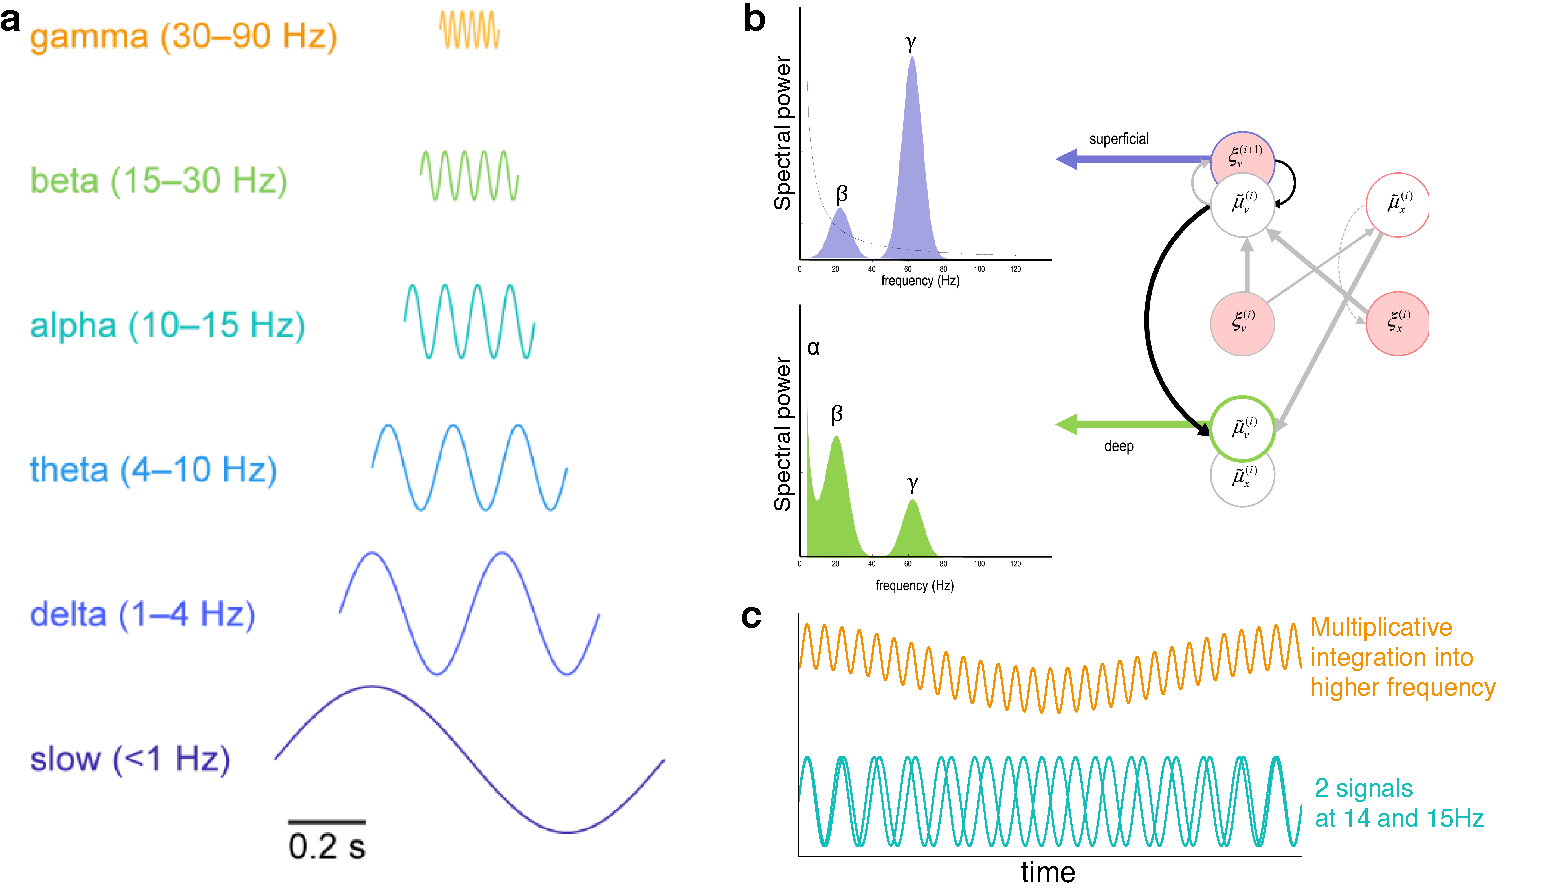
\includegraphics[width=1.\textwidth]{fig/fig_chap7_oscillations.pdf}
\caption[Neurobiological oscillations.]{Neurobiological oscillations and predictive coding. (a) Frequencies of oscillations found in neurobiological recordings. (b) Types of oscillations posited by a predictive coding neural network, from~\cite{bastos2012canonical}. (c) Illustration of the multiplication of two alpha-band predictive signals into a gamma-band prediction error.}
\label{fig_chap7_oscillations}
\end{figure}% oscillation figure + bastos frequencies + nonlinear mixtures (with the sine mixing)

The picture becomes more complex when one needs to understand that resolution of erroneous predictions through propagation of errors are not instantaneous. Predictions, fundamentally, should be based on the multimodal interactions of cortical areas, but also of multi-features interactions within a single modality. Practically, a prediction about a high-variance Motion Clouds is the interaction between multiple prediction error units, each signaling a single edge.

This means that the message passing in predictive coding occurs through a series of nonlinear transformation, implying that many alpha range signals will be transformed into higher frequency through this exchange. This summed interaction is often assigned to the second most prominent range of communication in the brain, gamma-band ($40 Hz$). Prediction errors, as they are based on this non-linear mixtures of expectations, must be present in those higher frequencies. Predictions, as they are more stable and need not be updated constantly (which forms the defining principle of predictive coding), should be only found in lower frequency. This "spectral asymmetry" of cortical communication~\cite{bastos2012canonical, bastos2015visual} explains many attentional mechanisms~\cite{kok2012attention}. This is also replicated with minimal assumption in silico, by showing that coupled neuronal oscillators with biological time constants, i.e. conduction delays of $12$ ms and synaptic time constant of $20$ ms naturally create an emergent alpha/gamma prediction/error oscillation.

It follows that spectral asymmetry also implies (functional) anatomical asymmetry, namely in the canonical model that predictions can be found in deep layers~\cite{bastos2012canonical}. Thus, given the anatomy of the corticothalamic projections, it would seem that predictions only are sent to the pulvinar. This effectively allows it to regulate which prediction of a given level of the visual hierarchy is best suited to provide the best explanation for an external sensory cause, based on its precision. This is specifically the theoretical principle we discuss in this article, by showing how alpha (predictive) rhythms in the pulvinar are gated by cortical activity.



\section{Article: "Corticothalamic Projections Gate Alpha Rhythms in the Pulvinar"}
This theoretical article discusses the role of synaptic asymmetry from the cortex to the pulvinar, so called corticothalamic terminals, and their role in communication between cortical areas. Two types of these terminals, originating from different hierarchical levels of the visual hierarchy, exhibit unique anatomical and functional patterns, causing distinct oscillatory rhythms in the pulvinar. Through a modeled cortical feedforward network including areas 17 (\gls{V1}) and 21a (V4), we found that these terminal types play antagonistic roles in regulating oscillatory activities in the pulvinar. We suggested that the varying activation of these terminals can gate the pulvinar responses, influencing the oscillatory transfer between lower and higher-order areas, ultimately impacting the neuronal communication throughout the cortical hierarchy. While not emphasized in the article to keep a coherent narrative, this can be interpreted as having a centralized nucleus of the visual network, the pulvinar, ascribing inverse variance weighting to cortical activity in order to modulate the message-passing between alpha (predictions) and gamma (predictions errors) activities. 

Full citation is as follows: \fullcite{cortes2021corticothalamic}
% avant d'intégrer un article dans votre thèse, consulter http://www.sherpa.ac.uk/romeo/ si vous souhaitez diffuser sur internet
\includepdfset{pagecommand=\thispagestyle{scrheadings}} % ajoute la numérotation continue des pages aux fichiers pdf importés
\includepdf[scale=0.82,pages=-]{papers/frontiers.pdf} % 'scale' ajuste la taille du pdf, vous pouvez affiner en fonction des marges



\section{Conclusion}
In this section, we explored the complex functional relationship between the pulvinar and \gls{V1}, with an emphasis on the regulatory processes associated with inverse variance computations. 

The anatomy of the pulvinar seems to be uniquely well-posed for inverse variance modulations in the visual hierarchy. Indeed, the functional connectivity is strictly modulatory from pulvinar to \gls{V1}, meaning that transthalamic connections could regulate prediction errors based on inverse variance right at the lowest level of the hierarchy. This modulatory activity likely has the role of preventing imprecise sensory inputs from propagating in the hierarchy, thus preventing them from updating (wrongly) an internal predictive model due to unreliable sensory input, which is very fitting with the gating role commonly assigned to the pulvinar~\cite{purushothaman2012gating}. Further, the asymmetrical nature of this connectivity between facilitating (type 1) and depressing (type 2) synapses, established as a function of the cortical hierarchy, fits very nicely with hierarchical Bayesian inference. In practice, this means that the pulvinar can compute a global associative signal linked to multiple level of inverse variance through the visual areas, and explain away irrelevant visual features. Deficit in this role, intuitively, can be conceptualized as propagation of irrelevant prior predictions, which is often reported in pulvinar lesion studies~\cite{robinson1992pulvinar}. 

The propagation of precision-weighted prediction and errors is also likely supported by neuromodulatory mechanisms that control synaptic gain, namely cholinergic signals~\cite{moran2013free}. As with the pulvinar, this mechanism provides a way to encode information related to environment through the excitability of circuits signalling prediction errors~\cite{keller2012sensorimotor}. In line with our results, this further aligns very well with the idea that superficial pyramidal cells are equipped with numerous synaptic gain control systems neuromodulatory receptors. Further, the clear effect of neuromodulatory mechanisms on synchronous activity in the cortex, and on alpha oscillations, hints at an interconnected mechanism throughout multiple neuronal levels~\cite{brown2007abnormal}.

Including such transthalamic and neuromodulatory connectivity in our view of the cortex is an important consideration, and this section offered a brief divergence to add some much needed mesoscale context to our results. We will now revisit, in the concluding section of this manuscript, cortical-centric computations enriched by an understanding of the hierarchical interplay afforded by the pulvinar. We posit that the pulvinar's interaction with cortical regions represents a second-order mechanism for implementing inverse variance computations in the brain, a theme we will expand upon when synthesizing the multiscale findings in the next chapter.



	\chapter{Conclusion}
\begin{flushright}
    \textit{''Well, I'm all for leaving \\
            and that being done,\\
            I've put in a request to take up my turn.''}\\
    Jethro Tull, A Passion Play, 1973
\end{flushright}



\section{Concluding Overview}
\subsection{Final Summary}
As the author of this manuscript easily recognized during proofreading, sifting through more than two hundred pages of early-career neuroscience is not exactly a straightforward ordeal. Although an attempt has been made to lower the attentional overhead involved in this reading by humoring the reader and by limiting the number of abbreviations, it is likely that days have elapsed between the beginning and the end of one's reading. As such, we would like to summarize, once last time, this manuscript

We first introduced the problem of inverse variance computations in vision by adopting a Marr-like approach in chapter 2. This introduced a study of the nature of natural images in chapter 3, exploring the trade-off between fidelity and sparsity, and their respective advantage when computing variance-bound probability distributions. 
This concept was pursued in chapter 4 in an electrophysiological study, leading to major contributions in terms of the functional role of cortical recurrence in computations of variance. 
%chapter 5 presents a novel model that integrates variance within the predictive coding framework, showcasing its prowess in image classification and generation tasks. This chapter also postulates a canonical intracortical variance computation that is repeated across different cortical areas. 
We then built further on these concepts in chapter 5, introducing cyclic computational graphs and reinforcing the idea of a multiscale model of orientation selectivity.
This was then extended in chapter 6, focusing beyond \gls{V1} and delves into the subcortical pathways, particularly highlighting the role of the pulvinar in managing variance in visual processing. Preliminary results from extrastriate cortical areas also hint at their potential involvement in variance computations.
Now, in chapter 7, we propose a (short) reflective summary, pondering the broad implications of these results for neuroscience and related fields. If the reader has any courage left, they are also provided with optional appendices that provide a deeper dive into the mathematical underpinnings of the free energy principle, as introduced at the beginning of this manuscript. The last appendix also includes supplementary material related to public communications surrounding this thesis.



\subsection{Towards a Coherent Model of inverse variance-weighting}
By nature, this manuscript encompasses a broad number of topics, including sparse coding, extracellular electrophysiology, artificial deep neural networks, graph theory, and thalamocortical communication. Rather than subject of studies in themselves, these were more designed as means towards an end - or rather, as hammers for one single nail (maybe spike, in our context). By giving coherent and convergent observation of the computations of inverse variance as based on recurrence, these contributions must now be framed in a single coherent framework.

Based on our results, we propose the following. The computation of inverse variance starts with the notion that the goal of primary sensory areas is to extract invariant representations of the world~\cite{keller2018predictive, barlow1961possible}. This might seem semantically contradictory, but if representations are to be invariant, then they must be encoded alongside an associated variance in the brain's internal models. Both under predictive coding or sparse coding, the goal of these internal models system is to build a representation of the world whilst enforcing the cost/efficiency tradeoff. In chapter 3, we show that the low-level invariant representations of natural images are oriented edges with factorized variance. A model of the visual world can rely on two strategies: encoding a distribution of edges using multiple single units (accurate, but not sparse) or encoding a distribution of edges using one unit, that encodes both median and variance (not necessarily accurate, but sparse). This latter scheme seems to be used, and can be likened to a Maximum Likelihood Estimation in the context of the Bayesian Brain (see Equation~\ref{eq_MLE}). In chapter 4, we show that both strategies are likely implemented in the neural substrate: many neurons that encode single edges, through a fast first pass in vulnerable neurons, a representation which then becomes a sparse but approximate estimate of variance in resilient neurons. In chapter 5, we also view this as a dynamically modulated (by variance) message passing through many neurons carrying different orientation information, creating a local, recurrence-based, strategy for encoding orientation variance.

Given that this computation can be created solely by local intra-area recurrence, it's likely running locally in parallel in every single cortical area. Quite probably, it is also running in every cortical area, visual or not. Thus, there must be a system of communication between these local processes that allows to regulate the flow of information based on these multiple inverse variance computations. Having a central modulator of these computations, in the form of the pulvinar, which controls propagation of (alpha-oscillating) predictions as shown in chapter 6, proves to be computationally advantageous and conceptually elegant. The longer time constants of this large-scale thalamocortical networks can also implement the computation of inverse variance through time, as discussed in chapter 6, which is also supported by empirical evidences of attention-deficit due to pulvinar lesions. It is likely that neuromodulator mechanisms are also involved~\cite{moran2013free}, which could be the brain-wide equivalent of the role the pulvinar is fulfilling for the visual cortex.
This constitutes our main scientific contribution, which, to quote the title of this thesis, is \textit{"A multiscale model to account for orientation selectivity in natural images"}.%, schematized in Figure~\ref{fig_chap8_megamodel}. 

%\begin{figure}[h!tbp]
%\vspace{0.1cm}
%\centering
%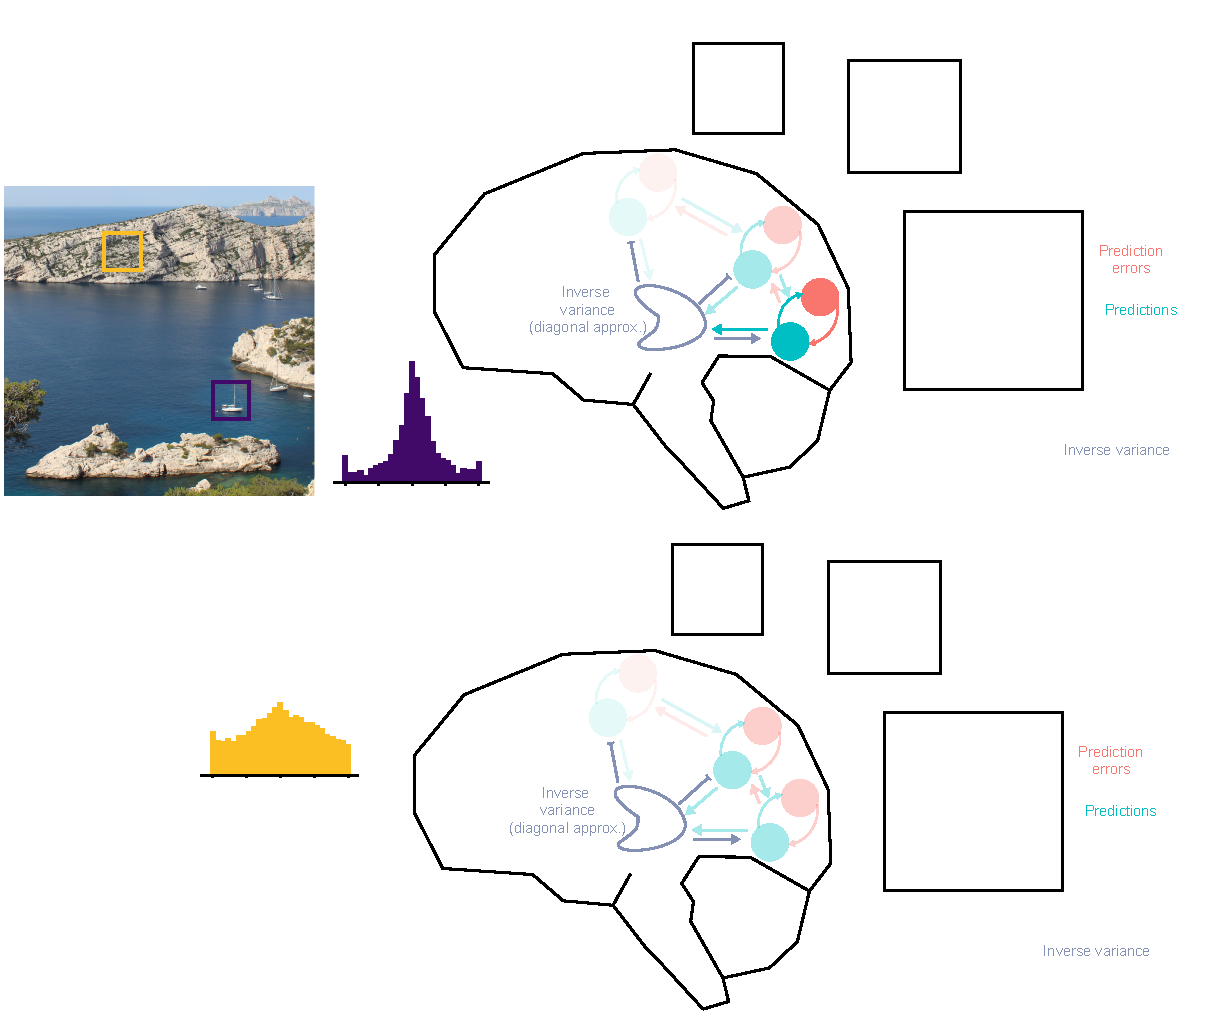
\includegraphics[width=1.\textwidth]{fig/fig_chap8_megamodel.pdf}
%\caption[Active modulation of neurons by orientation variance.]{Modulation of tuning curves by orientation variance. TODO.}
%\label{fig_chap8_megamodel}
%\end{figure} % figure that encompasses everything

This conceptual model also speaks to a number of testable hypotheses that can pave the way for exciting future research perspectives. But first, let us review the possible interpretations of this work, under both at the neurobiological and the computational front.



\section{Interpretation}
Although neuroscience has been historically based on studies related to how neurons encode only scalar approximate representations of their environment~\cite{sherrington1906observations, hubel1959receptive, o1971hippocampus}, theoretical~\cite{barlow1961possible} and experimental~\cite{leon2012motion} convergences have made it possible to start considering the full statistical nature of the environment we live in. The current research on inverse variance-weighting in the brain has exciting fundamental and clinical perspectives, which relates to two major avenues of interpretations. 



\subsection{Neurobiological Relevance}
At its core, inverse variance-weighting addresses the essential balance between internal priors and external perceptions. In the context of predictive processing, this mechanism guides the brain in discerning which of its predictions are reliable, and which it should discard in favor of prediction errors which warrant new attention. Interestingly, this dynamic can be seen as a foundational descriptor for several psychiatric disorders~\cite{friston2023computational}, including autism and schizophrenia.

\begin{figure}[h!tbp]
\vspace{0.1cm}
\centering
\includegraphics[width=1.\textwidth]{fig/fig_chap8_autism_schizo.pdf}
\caption[Message passing and computational psychiatry.]{Computational psychiatry under predictive processing.
(a) Message passing in the hierarchical Bayesian visual cortex. Under abnormally high inverse variance of the prior (second row), posterior is driven towards the internal models. Oppositely, high inverse variance of prediction errors (third row), drives posterior towards the sensory input. These respectively account for positive symptoms in schizophrenia and autism. 
(b) Same as (a), but in terms of bottom-up and top-down message passing, reproduced from~\cite{alamia2023oscillatory}.}
\label{fig_chap8_autism_schizo}
\end{figure} % figure for the inverse variance modulation + almia figure 1 from schizo paper

First, on a clinical level, recall that in the introduction (Figure~\ref{fig_chap2_equi_proba_var}), we discussed the notion that the variance of either prediction or prediction errors could drive the posterior likelihood towards one or the other. Under that generic description, hypersensitivity to external inputs, as is present in autistic spectrum disorders, can be conceptualized as a condition that drives overly precise prediction errors, overriding any possible internal models of the world. Typically, overlooking prediction error with no consequence for our inner model is something that we all do on a daily basis. In complex but non-threatening scenarios like social interactions, some errors are acceptable for broader understanding, and are part of the human social basis for learning. Inflexible processing of prediction errors in autism, due to impossibility of lowering their inverse variance-weighting in the decision process, leads to inability in ensuring "predictive success in an unpredictable world"~\cite{van2014precise}.

On the other end of the possible symptoms captured by inverse variance models lies schizophrenia. Hallucinatory experiences and feeling of disconnection with the external world~\cite{insel2010rethinking} are the hallmark of high weighting given to internal models over external likelihoods~\cite{sterzer2018predictive}. This is further supported by evidences that many of these symptoms align closely with the lesions of the neural substrate we described here, notably, visual perception and visual cognition being affected by pulvinar lesions~\cite{dorph2017postmortem}. Functional connectivity in schizophrenic patients have revealed reduced connectivity between the medial pulvinar and the frontal cortex~\cite{penner2018higher,yamamoto2018aberrant}. In the general model proposed earlier in this thesis, this would mean a compromised ability to regulate the flow of neuronal information between cortical areas by means of inverse variance weighting. Conversely, it could provide an evolutionary basis for the need for a central structure involved in the regulation of this mechanism, with a size proportional to that of the cortical areas being regulated~\cite{casanova2004functions}.

Second, on a cognitive level, another contribution of this thesis is to also offer a shift of our understanding of attention mechanisms, envisioning them as inverse variance mechanisms. Instead of conceptualizing recurrence and lateral inhibition as neural basis for sensory sharpening, one could consider that these are instead sampling mechanisms to drive (local) emphasis on the optimal percepts. 
Under this view, an interesting link is also to be made with the neuromodulatory activity, classically related to attention. Dopamine, for instance, is suggested to be crucial for the precision-adjustment of prediction errors, which in turn signals the significance of sensory inputs~\cite{fiorillo2008temporal, schultz1997neural}. Other neuromodulatory mechanism, such as cholinergic systems, can increase the gain of cortical neurons in response to sensory inputs~\cite{vaucher1997cholinergic, brown2011active}, and are thus tied to attentional mechanisms~\cite{kang2014boosting}. In that sense, these systems could be thought of as a third-order implementation of modulation by inverse variance, right after the first-order local recurrent interactions, second-order vision-centric pulvinar pathways, and serving to implement diffuse cortex-wise computations of inverse variance. 

Third, on a fundamental level, the dynamics of the activities that have been examined so far, as well as their propagation methods, their intracortical nature, all point towards an exciting research perspective for travelling waves. As introduced in chapter 4, traveling waves represent the dominant way of propagation of activity within the cortex. These waves facilitate processes like priming and suppression, but their exact role remains somewhat ambiguous and polymodal~\cite{muller2018cortical}. Similarly to the idea of a cholinergic mechanism, travelling waves also modulate the excitation/inhibition balance of the cortical activity rhythmically, which gates perceptual inference~\cite{dugue2011phase}. At the cortical area level, one contribution of this thesis is to consider that these waves might also implement a local inverse variance-weighting phenomenon, which offers a fresh perspective on their function in the cortex. At the macroscale, waves travelling between cortical areas, could also reveal mechanisms of propagation of inverse variance-weighted message, controlled by a series of locally weighted predictive oscillators~\cite{alamia2019alpha}. Specific changes in inverse variance could lower the excitability of prediction error units in the lower end of the hierarchy (i.e., in \gls{V1}), which would increase the preponderance of backward traveling waves, and correlates nicely with attentional experiments~\cite{alamia2019alpha}. One limitation here is that we have chosen to limit ourselves to an alpha/gamma duo, which is an oversimplification, and does not consider the fact that attentional visual search tasks correlates with even lower frequency rhythms, like theta~\cite{senoussi2019attention, michel2022distinct}. Given the tight relationship between unpredictable environment and the need for attentive search in feature space, this offers an interesting experimental perspective on manipulating visual variance, and correlating neural activity at the scale of the brain with the need to drive away - or close to - the input likelihood from posterior distributions. This will be discussed further in the final section of this manuscript.



\subsection{Machine Learning Relevance}
Inverse variance-weighting plays a significant role in both statistical and machine learning research~\cite{murphy2012machine}. Under this interpretation, inverse variance provides distinct advantages to a model, without implementational drawbacks (as studied in the neuroscientific context here). Indeed, given the mathematical triviality to compute a correlational matrix and inverse it, modelers obtain all the theoretical advantages described so far, with none of the complications related to recurrent neural message passing. One key advantage of implementing a degree of variance to a model's decision is to allow the readout of the model's confidence in its output. This can be as straightforward, in a deep neural network, as computing the sum of the variances in all layers, such that a network that has learned a precise representation of the environment returns a globally low variance of its activity.

Recently, the importance of associating confidence levels with algorithmic decisions has grown, placing inverse variance-weighting at the forefront of machine learning algorithm development. While there might be lighthearted examples, such as deep learning models mistakenly classifying an image of a panda with a single modified pixel as a dog, the stakes are much higher in practical industrial applications. As the research shifts towards implementing safety-critical neural networks, the emphasis on variance-weighted decisions becomes paramount. To quote Kendall and Yarin~\cite{kendall2017uncertainties}:  
\begin{flushleft}
    \textit{''Mappings are often taken blindly and assumed to be accurate, which is not always the case. In (\ldots) recent examples, this has had disastrous consequences. In May 2016 there was the first fatality from an assisted driving system, caused by the perception system confusing the white side of a trailer for bright sky. If (\ldots) these algorithms were able to assign a high level of uncertainty to their erroneous predictions, then the system may have been able to make better decisions and likely avoid disaster.''}\\
    from \fullcite{kendall2017uncertainties}
\end{flushleft}

Incorporating explicit learning rules based on variance into data modeling undeniably introduces additional complexity. As we have shown in the introduction of this manuscript and in the conclusion of chapter 5, these merely require simple additional considerations, and are compatible with current neural network frameworks. In that note, leading Deep Learning frameworks have already integrated support for Bayesian learning~\cite{paszke2017automatic}, which are soon bound to overtake regular Deep Learning in popularity~\cite{baldwin2022deep}.

A promising pathway to bridge explicit variance learning rules and neurobiology lies in predictive coding models. These models empirically approximate gradient backpropagation, a cornerstone technique for training deep neural networks (see chapter 3), across arbitrary computational graphs~\cite{millidge2022predictive}. This suggests that practically any deep neural network could be trained using units dedicated to predictions and their errors. Practical applications of this theory are already evident in simpler datasets like MNIST~\cite{millidge2020relaxing}. Notably, as we detailed in the conclusion of chapter 5, the implementation of inverse variance-weighting in this context is a novel proposition, as identity matrices are often use for simplicity's sake. The programming of these networks is elegantly simple - less than 100 Python code lines for an implementation as mathematically framed here~\cite{millidge2020relaxing}. On modern hardware, they also achieve comparable accuracy and convergence speeds to traditional backpropagation techniques.

Moreover, predictive coding's use in causal inference (as a generative model) could shed new light on how neural networks simulate and analyze dynamics within their nodes. In the recent context of Large Language Models, the inherent flexibility of predictive coding models allows any unit in the network to be set as a latent variable, endowing these models with the ability for flexible internal conditioning. This would enhance steerability over the network, for desirable safety purposes. The generative nature of these models also equips them to deal with incomplete inputs or outputs, a situation which typically requires expensive data curation by humans in the context of Deep Neural Networks. This attribute could be advantageous in creating models that infer missing information seamlessly. Finally, predictive coding also extends in a rather straightforward manner to arbitrary time-space variables, which allows for dynamical modelling, something which backpropagations techniques have always struggled with~\cite{millidge2022predictive}.

In the realm of hardware, the benefits of employing variance weighting through lateral inhibition might mirror those observed in neurobiology. Specifically, this method can offer computational allocation for significant, unpredictable fluctuations in data, while concurrently diminishing or sidestepping routine, predictable data streams. Highlighting these pronounced shifts could streamline the data transmitted across physical conduits, addressing a primary source of heat and computational inefficiency in neuromorphic chips~\cite{eshraghian2022memristor, rahimi2020complementary}. This could lead to faster, more energy-efficient neuromorphic networks that are particularly useful for edge computing, which, arguably, might also be why they are also implemented in the first place in the brain. Such asymmetrical message-passing structure is also reflected in the activity of \gls{V1}, notably, in the rasterplots presented in chapter 4.



\section{Limitations of the Studies}
The elaboration of a doctoral manuscript requires the doctoral candidate to perform scientific work, but also to learn how to even do such scientific work in the first place. As such, the erudite reader might have already spotted a number of suboptimal procedures in the experiments which are intrinsically bound to the learning curve the author went through. On a positive note, none of these limitations are unsurmountable roadblocks, and most of them can serve to formulate useful hypothesis for future research directions.

First and foremost, there is an intrinsic limit in the interpretations one can give from the experiments carried in chapter 4. Such extracellular recordings were performed under anesthesia, which yields heavy modulations of the activity of neurons~\cite{villeneuve2003use}. We have addressed this limitation in the conclusion of chapter 4's article, citing examples of experiments that were successfully translated from anesthetized to awake animals. One key neurophysiological element is however missing. Convincing experimental proofs have been published during the thesis, showing that the main effect of anesthesia is to decouple basal and apical dendrites of layer V cortical neurons~\cite{suzuki2020general}. Further, since pharmacological agents modulating the internal representations of the brain (i.e., predictions) have been shown to target specifically these same neurons~\cite{heindorf2022reduction}, it seems evident that one part of the prediction/prediction error network was heavily modulated in our experiments. Carrying experiments in awake, vigil animals is one way to address this limit, and the experiments in chapter 5 are a fair proof that chapter 4's study can yield interesting insights into a more ecologically relevant setting.

However, these experiments were carried with Utah Arrays (see chapter 4 and 5), which means a complete loss of information of the laminar position of neurons recorded. As such, we currently have no proof of a laminar-dependent inverse variance computations in awake cortex of primates. Change of coupling in deep layers might make for a very compelling case, which could be that inverse variance is also computed for predictions in layer V. Anatomically, there is actually as much, if not more (proportionally) recurrent connectivity between neurons of layer 5 of different neighboring cortical columns~\cite{briggs2011corticogeniculate, bastos2012canonical}. Functionally, layer V recurrent interactions also support very complex types of computations\cite{velez2014stimulus}, which are unique to these layers (some similarities exist~\cite{galloni2020apical}). This fully-lateral model of the cortex will be the central point of future research direction, and will be discussed in the next Perspectives section. 

Second, the choice of recording local, laminar, extracellular potentials is clearly not ideal for studying recurrent interactions. Using a better suited method would have required to know beforehand that recurrent interactions can carry out inverse variance weighting in the cortex, which was only hinted at by speculative models~\cite{bastos2012canonical, friston2005theory}. As such, a vast portion of neuronal "dark matter" was not observed, but only inferred. In a sense, this serves the interdisciplinar argument of this manuscript, which uses computational models to overcome experimental limitations. Now that these recurrent principles have been fairly well established, optical methods would be much better suited to study the inverse variance weighting mechanism in the cortex. One could expect some very interesting parallels between the results presented here, and the travelling waves (see chapter 4) observed both at the cortical area scale~\cite{chavane2011lateral} and at the brain scale~\cite{muller2018cortical, alamia2019alpha}. In terms of dynamics, travelling waves propagate locally with speeds that are coherent with the idea of a series of iterative recurrence-based computations~\cite{chavane2011lateral, chavane2022revisiting}. This possesses interesting ties with predictive processing, because local recurrence can allow a visual map to predict future position of a moving object through local interactions~\cite{britten1992analysis}, which is actually embedded within a travelling wave~\cite{benigno2023waves}. This experimental limitation, and its possibles interpretations in terms of travelling waves, will form part of the research perspectives discussed in the next section. 

%Third, there exists a limit in the assumptions used in the mapping of neurobiological elements for predictive processing. Since the inception of this thesis, there has been convincing biological experiments showing that prediction errors units are not only present in supragranular layers~\cite{keller2018predictive}, but also in deeper layers~\cite{heindorf2022reduction}. This could call for a major revision of the classical Bastos microcircuit model~\cite{bastos2012canonical}, which segregated the prediction and prediction errors to distinct layers, towards a model with duplicated compartments that essentially give the network a "teaching" signal for each cortical area, duplicated across layers % this makes no fucking sense but then again i've commented it out. the idea is that you duplicate the PE/P circuit twice so that you double the layer, and L2/3 serves to run a putative model of the environment that drive a predictive model int he deeper layers



\section{Perspectives for Future Research}
To conclude this thesis, we will develop here two major research perspectives that have stemmed from the present findings, and that are actively under study at the time of this writing. The first perspective stems from chapter 4 and 5 experiments, and concern extension of this thesis' work to rodent models. The second perspective is more ambitious, and better suited for exploration during a post-doctoral tenure. Both trajectories engage with the notion that existing models of recurrent connections in the cortex may be either limited by primate-centric considerations, or could simply be fundamentally unable to account for the meso-scale implementation of message passing in the cortex.

\subsection{Precision-Weighting without an Orientation Map}
The take-home message of this manuscript is that recurrence between specifically clustered groups of cells in orientation space mediates the computation of the inverse variance of orientation in \gls{V1}. But, how can these computations take place when there is no such thing as a specifically clustered groups of cells ? This is a non-trivial question, as this seemingly random architecture constitutes the organization of rodents' salt-and-pepper \gls{V1}. While primates and felines have clustered orientation processors organized in a map, which emerges through their heavy reliance on vision, rodents instead rely on whisker sensing, and thus lack a topologically structured orientation selective activity. Their somatosensory cortex, which processes information from the whiskers, do follow a topological structure. The extension of inverse variance-weighting in rodent cortex could be achieved by designing a class of stimulus similar to Motion Clouds, in the texture domain, and observe whether the variance-weighting in \gls{V1} holds in the somatosensory domain.

Back to the visual cortex, preliminary results from the co-authors Lamyae Ikan and Nelson Cortes suggest that mice do not exhibit any type of resilience to increased sensory variance, contrary to felines (chapter 4) and primates (chapter 5). If we put this under the notion that structured cortical recurrence is needed for such computations, this is one more argument in favor of this thesis' hypothesis. If we put this in the general predictive coding notion that high variance input are "explained away" and do not update the model, then it would be interesting to see what happens behaviorally. Even without processing of variance, does Bayesian inference still occur, and does the animal discard entirely its sense of vision to rely on its whiskers ? 

This also speak to an interesting property of resilience to general sources of uncertainty, as opposed to solely variance. Rodents do not possess orientation maps, but do possess individual neurons strongly tuned to specific orientations, with functional properties such as contrast invariance like primates~\cite{finn2007emergence}. This shows that an orientation map is not crucial for feature sensitivity, nor for maintaining contrast invariance. Changes in contrast, much like changes in orientation variance, are a source of visual uncertainty. Both type of uncertainty seem to affect \gls{V1} in the same way, at least in the pionnering study of Goris et al.~\cite{goris2015origin} (see also Figure~\ref{fig_chap8_mouse_mc}.
There is then a discrepancy between the notion that activity in primate \gls{V1} is similarly influenced by uncertainty of orientation (variance) and luminance (contrast), and the fact that mice are resilient to the latter but not the former. Contrast invariance mechanisms are a very popular topic in visual neuroscience, and there exists many theories on the emergence of contrast-invariant activity in \gls{V1}~\cite{vidyasagar2015origins}. While some authors suppose that cortical interactions could create contrast invariance~\cite{troyer1998contrast}, others have supposed that non-linearity in the thalamo-cortical connections from the \gls{LGN} is responsible for contrast invariance~\cite{finn2007emergence}. It would seem that, given this uncoupling between variance and luminance, the latter hypothesis would be better supported by our results.

\begin{figure}[h!tbp]
\vspace{0.1cm}
\centering
\includegraphics[width=1.\textwidth]{fig/fig_chap8_mouse_mc.pdf}
\caption[Contrast and orientation invariance in mouse\gls{V1}.]{Contrast and orientation invariance in mouse \gls{V1}. (a) Salt-and-pepper organisation of \gls{V1}, from~\cite{jang2020retino}. (b) Similar effect of contrast and orientation invariance on two primate \gls{V1} neurons, from~\cite{goris2015origin}. (c) An example of non-linear gain model that accounts for contrast resilience in \gls{V1}, from~\cite{finn2007emergence}. (d) Example of mice \gls{V1} neurons, showing a massive decrease in firing rate (arrows) with increased orientation variance (courtesy of Nelson Cortes). }
\label{fig_chap8_mouse_mc}
\end{figure} % figure about salt and pepper maps, contrast invariance


\subsection{The Microcircuit is Dead, Long Live the Microcircuit}
The theoretical framework upon which we have built our hypotheses, predictive processing~\cite{rao1999predictive,friston2005theory}, offers a solid mathematical basis to understand cortical functions. The accurate mapping of theory to biology, however, remains speculative~\cite{bastos2012canonical,shipp2016neural}, aside from accurate understanding of the prediction error circuits~\cite{keller2012sensorimotor, keller2018predictive}. Recall that earlier in the text, we mentioned recent findings by Heindorf and Keller~\cite{heindorf2022reduction}, who, utilizing antipsychotics and widefield calcium imaging in behaving mice, have demonstrated that antipsychotic drugs selectively impact Layer 5 neurons. As antipsychotics should target the neural elements responsible for internal representations~\cite{friston2018does} (i.e., predictions), this argues in favor of Layer 5 as the seat of predictions in the cortex. This is in line with the speculative layout of predictive coding in the cortical microcircuit~\cite{bastos2012canonical} (Figure~\ref{fig_chap2_microcircuit}). Yet, the effect of antipsychotics is selective to Layer 5, and leaves superficial layers unaffected. This poses a significant challenge to the established model of a series of hierarchically organized vertical microcircuits, derived from the columnar model of the cortex (Figure~\ref{fig_chap8_lateral}).

Namely, the canonical microcircuit~\cite{martin1994brief} posits an input in Layer 4, followed by a processing in Layer 2/3, which is then sent to a higher order cortical area's Layer 4. This challenge is not recent, as the vertical microcircuit as always had scientific opposition~\cite{horton2005cortical}, mostly on functional basis. Support for a new "horizontal microcircuit" perspective is now further bolstered by anatomical studies, which revealed a bidirectional flow of pathways segregated into two supra- and infragranular streams~\cite{markov2014anatomy}. This makes intuitive evolutionary sense, given that the appearance of six cortical layers is thought to result from a duplication of a three-layered structure~\cite{shepherd2011microcircuit}. It thus becomes increasingly plausible that neural activity is focused on integrating disparate features to construct probabilistic representations of the environment, rather than integrating information within a vertical microcircuit. This is evidenced not only by the fact that horizontal communication is the dominant mode of the cortex~\cite{muller2018cortical}, but also by the fact that inverse variance weighting requires a horizontal (recurrent) communication system~\cite{ladret2023cortical}.

\begin{figure}[h!tbp]
\vspace{0.1cm}
\centering
\includegraphics[width=1.\textwidth]{fig/fig_chap8_lateral.pdf}
\caption[Towards a horizontal microcircuit.]{Towards a horizontal microcircuit. (a) Canonical microcircuit of \gls{V1}~\cite{martin1994brief} (top) and assumed but wrong serial communication between area (bottom). (b) The cortex instead projects in two counterstreams that densely connect every area to one another. Adapted from~\cite{markov2014anatomy}. (c) Recording from a Genetically Encoded Voltage Indicators correlate with silicon probes, as used in this thesis, allowing for KHz-fast widefield imaging of the communication throughout the cortex, from ~\cite{lu2023widefield}.}
\label{fig_chap8_lateral}
\end{figure} % figure about salt and pepper maps, contrast invariance

In light of these evidences, it is essential to address the implications they hold for the cortical model of the canonical microcircuit, particularly as they propose both an extension and a challenge to the results of this thesis. If Layer 5 neurons have been affected due to anesthetic decoupling, as proposed above ~\cite{suzuki2020general}, the impact of this experimental limitation is more significant than previously thought. These neurons might not have just been part of a vertical microcircuit, but could have been an integral component of an independent horizontal deep circuit altogether, with an independent recurrent dynamic. Additionally, the manipulation of the variance of Motion Clouds and sensory inputs might have focused the present work on the inverse variance-weighting of prediction errors, rather than a combined investigation that includes both prediction errors and sensory inputs. This focus could have led to the inability to read out input variance from deep cortical layers in chapter 4. If we wish to amend this, there is an intrinsic technological challenge for current research methods of investigation (Figure~\ref{fig_chap4_chemla}).

Sampling the recurrent activity of inverse variance-weighting throughout the cortex, not at the scale of a single area, but at the dominant scale of cortex-wide activity, requires an experimental paradigm shift. This involves sampling widefield activity at the Nyquist frequency of the fastest signals required, i.e., $\approx 50$Hz gamma-band prediction errors (Figure~\ref{fig_chap7_oscillations}).
The advent of advanced optical methods now permits kHz-level recording of brain activity using Genetically Encoded Voltage Indicators. Wide-field microscopy techniques enable the observation of awake, behaving mice, granting comprehensive access to the visual cortex's surface. By employing genetically specific constructs, it is possible to isolate recordings to deep or superficial cortical layers~\cite{lu2023widefield}. Through such recordings of traveling waves, we can apply the vast body of literature on brain oscillations to living neural activity. 

This approach aligns with the theoretical models illustrated in Figure~\ref{fig_chap7_oscillations}, facilitating manipulation of the sensorium of behaving brains to pinpoint the anatomical seat of internal neuronal representations. Correlated with the known existence of prediction error circuits, this is the next scientific step for predictive coding, which has already achieved Marr's algorithmic~\cite{friston2005theory} and computational~\cite{sprevak2021predictive} levels, and is now poised to achieve implementational level, through a wholistic mapping of the neural elements of predictive coding.

	\appendix

	\newpage
	\printbibliography[heading=bibintoc]%% bibliographie
	
	\newpage
	\printindex							%% index
	
	\newpage
	\printendnotes						%% notes

	\setcounter{chapter}{0}
\renewcommand{\thesection}{\Alph{section}}

\chapter*{APPENDICES}
\newpage
\addcontentsline{toc}{chapter}{APPENDICES}

\section{Appendix A: Additional Equations} 
\begin{flushright}
    \textit{''I'm not a gentleman,\\
    I'm the (Material and) Method man.''}\\
    approximate quote from Wu-Tang Clan's Method Man, The What, 1994
\end{flushright}
\label{appendix_maths}

\subsection{Equation 2.9}
The full differentiation of $F$ over $\Phi$ serves no introductory purpose, and is thus left out of Chapter 2 - equation \ref{eq_dF_dPhi}. It is written here, as: 

$$ \frac{\delta F}{\delta \Phi} = 
\frac{1}{2} \left(
\frac{\delta}{\delta \Phi}     \left(-\frac{(u - g(\Phi))^2}{\Sigma_u}\right) +
\frac{\delta}{\delta \Phi}     \left(-\frac{(\Phi - v_p)^2}{\Sigma_p}\right) + 
\frac{\delta}{\delta \Phi}      \left( -\ln\Sigma_u \right) + 
\frac{\delta}{\delta \Phi}      \left( -\ln\Sigma_p \right) + 
\frac{\delta}{\delta \Phi}      C
\right)
$$

$$ = 
\frac{1}{2} \left(
\left( -\frac{1}{\Sigma_u} \frac{\delta}{\delta \Phi} (u-g(\Phi))^2) \right) +
\left( -\frac{1}{\Sigma_p} \frac{\delta}{\delta \Phi} (\Phi-v_p)^2 \right)
\right)
$$

Applying the power rule $(f(x)^n)' = n f(x)^{n-1} f'(x)$:
$$ = 
\frac{1}{2} \left(
\left( -\frac{1}{\Sigma_u} 2(u-g(\Phi))\frac{\delta}{\delta \Phi} (u-g(\Phi)) \right) +
\left( -\frac{1}{\Sigma_p} 2(\Phi-v_p) \frac{\delta}{\delta \Phi} (\Phi-v_p) \right)
\right)
$$

And then splitting the linear differentiation:
$$ = 
\frac{1}{2} \left(
\left( -\frac{1}{\Sigma_u} 2(u-g(\Phi)) \left(\frac{\delta}{\delta \Phi} u - \frac{\delta}{\delta \Phi} g(\Phi)\right) \right) +
\left( -\frac{1}{\Sigma_p} 2(\Phi-v_p) \left(\frac{\delta}{\delta \Phi} \Phi - \frac{\delta}{\delta \Phi} v_p \right)\right)
\right)
$$

$$ = 
\frac{1}{2} \left(
\left( -\frac{1}{\Sigma_u} 2(u-g(\Phi)) \left(0 - g'(\Phi)\right) \right) +
\left( -\frac{1}{\Sigma_p} 2(\Phi-v_p) (1+0) \right)
\right)
$$

$$ = 
\frac{1}{2} \left(
\left( -\frac{1}{\Sigma_u} 2(u-g(\Phi))(-g'(\Phi)) \right) +
\left( -\frac{1}{\Sigma_p} 2(\Phi-v_p) \right)
\right)
$$

$$ = 
\left( \frac{1}{\Sigma_u} (u-g(\Phi))(g'(\Phi)) \right) +
\left( -\frac{1}{\Sigma_p} (\Phi-v_p) \right)
$$

Simplifying and changing the order of the right-hand side term, we get:
$$ F = 
\frac{(u-g(\Phi))}{\Sigma_u} g'(\Phi)   +
\frac{(v_p-\Phi)}{\Sigma_p}  
$$

yielding equation \ref{eq_dF_dPhi}. 



\newpage 
\subsection{Equation 2.25}
For differentiating the terms $v_p, \Sigma_u \Sigma_p$ over $F$ for Equation \ref{eq_df_derror}, we start from the definition of $F$ as:
$$ F = \frac{1}{2} \left( - \ln \Sigma_p - \frac{(\Phi - v_p)^2}{\Sigma_p}  - \ln \Sigma_u - \frac{(u - g(\Phi))^2}{\Sigma_u}\right) + C$$

We will derive first for $v_p$:
$$ \frac{\delta F}{\delta v_p} =
\frac{1}{2} \left(
\frac{\delta}{\delta v_p} \left( - \frac{(\Phi - v_p)^2}{\Sigma_p} \right) +
\frac{\delta}{\delta v_p} \left( - \frac{(u - g(\Phi))^2}{\Sigma_u} \right) +
\frac{\delta}{\delta v_p} \left( - \ln \Sigma_u  \right) + 
\frac{\delta}{\delta v_p} \left( - \ln \Sigma_p  \right) + 
\right)
\frac{\delta}{\delta v_p} C
$$
$$ 
 = \frac{1}{2} \left(
\frac{\delta}{\delta v_p} \left( - \frac{(\Phi - v_p)^2}{\Sigma_p} \right) 
\right)
$$
$$ 
 = \frac{1}{2} \left(
\frac{1}{-\Sigma_p}
\frac{\delta}{\delta v_p} (\Phi - v_p)^2
\right)
$$

Using the power rule to eliminate both halved and squared terms:
$$ 
= 
\frac{1}{-\Sigma_p}
(\Phi - v_p)
\frac{\delta}{\delta v_p} (\Phi - v_p)
$$
$$ 
= 
\frac{1}{-\Sigma_p}
(\Phi - v_p)
\left(\frac{\delta}{\delta v_p} \Phi -
\frac{\delta}{\delta v_p} v_p\right)
$$
$$ 
= 
\frac{1}{-\Sigma_p}
(\Phi - v_p)
(0 -
1)
$$

$$ 
= \frac{\Phi - v_p}{\Sigma_p}
$$

Now once again, for $\Sigma_p$
$$ F = \frac{1}{2} \left( - \ln \Sigma_p - \frac{(\Phi - v_p)^2}{\Sigma_p}  - \ln \Sigma_u - \frac{(u - g(\Phi))^2}{\Sigma_u}\right) + C$$
$$  \frac{\delta F }{\delta \Sigma_p} = 
\frac{1}{2} \left(
\frac{\delta}{\delta \Sigma_p} \left( - \frac{(\Phi - v_p)^2}{\Sigma_p} \right) +
\frac{\delta}{\delta \Sigma_p} \left( - \frac{(u - g(\Phi))^2}{\Sigma_u} \right) +
\frac{\delta}{\delta \Sigma_p} \left( - \ln \Sigma_u  \right) + 
\frac{\delta}{\delta \Sigma_p} \left( - \ln \Sigma_p  \right)  
\right) +
\frac{\delta}{\delta \Sigma_p} C
$$
$$  = 
\frac{1}{2} \left(
- \frac{\delta}{\delta \Sigma_p} \ln \Sigma_p +
\left( - (\Phi - v_p)^2
\frac{\delta}{\delta \Sigma_p} \frac{1}{\Sigma_p} \right) 
\right)
$$
Applying $ \left(\frac{1}{f(x)}\right)' = - \frac{f'(x)}{f(x)^2} $, this becomes 
$$  = 
\frac{1}{2} \left(
- \frac{1}{\Sigma_p} +
\left(  (\Phi - v_p)^2
\frac{\frac{\delta}{\delta \Sigma_p} \Sigma_p}{\Sigma_p^2} \right) 
\right)
$$
$$  = 
\frac{1}{2} \left(
(\Phi - v_p)^2
\frac{\frac{\delta}{\delta \Sigma_p} \Sigma_p}{\Sigma_p^2} 
- \frac{1}{\Sigma_p}
\right)
$$
$$  = 
\frac{1}{2} \left(
\frac{1(\Phi - v_p)^2}{\Sigma_p^2} 
- \frac{1}{\Sigma_p}
\right)
$$
$$  = 
\frac{1}{2} \left(
\frac{(\Phi - v_p)^2}{\Sigma_p^2} 
- \frac{1}{\Sigma_p}
\right)
$$

The same is done for $\Sigma_u$: 
$$ F = \frac{1}{2} \left( - \ln \Sigma_p - \frac{(\Phi - v_p)^2}{\Sigma_p}  - \ln \Sigma_u - \frac{(u - g(\Phi))^2}{\Sigma_u}\right) + C$$
$$  \frac{\delta F }{\delta \Sigma_u} = 
\frac{1}{2} \left(
\frac{\delta}{\delta \Sigma_u} \left( - \frac{(\Phi - v_p)^2}{\Sigma_p} \right) +
\frac{\delta}{\delta \Sigma_u} \left( - \frac{(u - g(\Phi))^2}{\Sigma_u} \right) +
\frac{\delta}{\delta \Sigma_u} \left( - \ln \Sigma_u  \right) + 
\frac{\delta}{\delta \Sigma_u} \left( - \ln \Sigma_p  \right)  
\right) +
\frac{\delta}{\delta \Sigma_u} C
$$
$$  = 
\frac{1}{2} \left(
\frac{\delta}{\delta \Sigma_u} \left( - \frac{(u - g(\Phi))^2}{\Sigma_u} \right) -
\frac{\delta}{\delta \Sigma_u}   \ln \Sigma_u   
\right)
$$
$$  = 
\frac{1}{2} \left(
-(u - g(\Phi))^2 \frac{\delta}{\delta \Sigma_u}\frac{1}{\Sigma_u} -
\frac{\delta}{\delta \Sigma_u}   \ln \Sigma_u   
\right)
$$
$$  = 
\frac{1}{2} \left(
-(u - g(\Phi))^2 \frac{\delta}{\delta \Sigma_u}\frac{1}{\Sigma_u} -
\frac{1}{ \Sigma_u}
\right)
$$
Once more, using $ \left(\frac{1}{f(x)}\right)' = - \frac{f'(x)}{f(x)^2} $, we get
$$  = 
\frac{1}{2} \left(
(u - g(\Phi))^2 \frac{\frac{\delta}{\delta \Sigma_u} \Sigma_u}{\Sigma_u^2} -
\frac{1}{ \Sigma_u}
\right)
$$
$$  = 
\frac{1}{2} \left(
 \frac{(u - g(\Phi))^2}{\Sigma_u^2} -
\frac{1}{ \Sigma_u}
\right)
$$
$$  = 
\frac{1}{2} \left(
\frac{(u - g(\Phi))^2}{\Sigma_u^2} -
\frac{1}{ \Sigma_u}
\right)
$$

yielding all three equations \ref{eq_df_derror}.

\newpage 
\subsection{Equation 2.28}
For moving from the scalar to the matrix form of a predictive network, as done in Equation~\ref{eq_pc_matrix}, we increase the dimensionality of our toy model organism, which now has observed sensory input $\bar{u}$ and tries to estimate the most likely values $\bar{\Phi}$ of the variables $\bar{v}$. As before, this model has prior expectations that $\bar{v}$ comes from the multivariate normal distribution with mean $\bar{v_p}$ and covariance matrix $\mathbf{\Sigma_p}$. Thus:
$$
f(\bar{x}, \bar{\mu}, \boldsymbol{\Sigma}) = 
\frac{1}{\sqrt{(2\pi)^N|\boldsymbol{\Sigma}|}}
exp \left[ -\frac{1}{2} (\bar{x} - \bar{\mu})^T \boldsymbol{\Sigma}^{-1}  (\bar{x} - \bar{\mu}) \right]
$$
where $N$ is the length of the vector $\bar{x}$ and $|\Sigma|$ is the determinant of the matrix $\Sigma$. Hence we have:
$$
p(\bar{u} | \bar{v}) = f(\bar{u}; g(\bar{v}, \boldsymbol{\Theta}), \boldsymbol{\Sigma_u})
$$
where $\mathbf{\Theta}$ are the parameters of the function g.

Now we can write down the free energy $F$ as:
\begin{equation*}
    \begin{aligned}
        F &= \ln p(\bar{\phi}) + \ln p(\bar{u} | \bar{\phi}) \\
        &= \ln 
\left[
\frac{1}{\sqrt{(2\pi)^N|\boldsymbol{\Sigma_p}|}}
exp \left[ -\frac{1}{2} (\bar{\phi} - \bar{v_p})^T \boldsymbol{\Sigma_p}^{-1}  (\bar{\phi} - \bar{v_p}) \right]
\right] \\
&+
\ln 
\left[ 
\frac{1}{\sqrt{(2\pi)^N|\boldsymbol{\Sigma_u}|}}
exp \left[ -\frac{1}{2} (\bar{u} - g(\bar{\phi}, \boldsymbol{\Theta}))^T \boldsymbol{\Sigma_u}^{-1}  (\bar{u} - g(\bar{\phi}, \boldsymbol{\Theta})) \right]
\right]
    \end{aligned}
\end{equation*}

$\frac{1}{\sqrt{(2\pi)^N}}$ is a constant, which we group under a constant $C$ term:

\begin{equation*} % ptdr l'enfer a relire
    \begin{aligned}
        F &= \frac{1}{2}
        \left[
        \ln \left(
        \frac{1}{|\boldsymbol{\Sigma_p}|}
        exp  \left( -(\bar{\phi} - \bar{v_p})^T \boldsymbol{\Sigma_p}^{-1}  (\bar{\phi} - \bar{v_p}) \right)
        \right) \right] \\
        &+
        \frac{1}{2}
        \left[
        \ln \left(
        \frac{1}{|\boldsymbol{\Sigma_u}|}
        exp  \left( -\bar{u} - g(\bar{\phi}, \boldsymbol{\Theta}))^T \boldsymbol{\Sigma_u}^{-1}  (\bar{u} - g(\bar{\phi}, \boldsymbol{\Theta}) \right)
        \right)
        \right]
        +C \\ \\
        &= \frac{1}{2}
        \left[
        \ln \left(
        \frac{1}{|\boldsymbol{\Sigma_p}|} \right)
        +
        \ln \left( exp  \left( -(\bar{\phi} - \bar{v_p})^T \boldsymbol{\Sigma_p}^{-1}  (\bar{\phi} - \bar{v_p}) \right) \right) \right]\\
        &+
        \frac{1}{2}
        \left[
        \ln \left(
        \frac{1}{|\boldsymbol{\Sigma_u}|} \right)
        +
        \ln \left( exp  \left( -\bar{u} - g(\bar{\phi}, \boldsymbol{\Theta}))^T \boldsymbol{\Sigma_u}^{-1}  (\bar{u} - g(\bar{\phi}, \boldsymbol{\Theta}) \right) \right)
        \right]
        +C \\ \\
        &=
        \frac{1}{2}
            \left[
            - \ln (|\boldsymbol{\Sigma_p}|) -
            (\bar{\phi} - \bar{v_p})^T \boldsymbol{\Sigma_p}^{-1}  (\bar{\phi} - \bar{v_p}) -
            \ln (-|\boldsymbol{\Sigma_u}|) -
            (\bar{u} - g(\bar{\phi}, \boldsymbol{\Theta}))^T \boldsymbol{\Sigma_u}^{-1}  (\bar{u} - g(\bar{\phi}, \boldsymbol{\Theta}))
            \right]
        \\&+C
    \end{aligned}
\end{equation*}

As we will now express everything in matrix term, it is useful to remember some properties, such as the gradient on vectors:
$$
\bar{x} = 
\begin{bmatrix} x_1 \\ x_1 \end{bmatrix}
$$
if $ y = \bar{x}^T\bar{x} = x_1^2+x_2^2$ by construction, so the gradient becomes
$$
\frac{\delta y}{\delta \bar{x}} =
\begin{bmatrix} \frac{\delta y}{\delta x_1} \\ \frac{\delta y}{\delta x_2} \end{bmatrix} =
\begin{bmatrix} 2x_1 \\ 2x_2 \end{bmatrix} =
2\bar{x}
$$

Knowing that $\Sigma$ matrices are symmetric (because they are covariance matrices), we can now compute the gradient of:
$$
F = \frac{1}{2}
\left[
- \ln (|\boldsymbol{\Sigma_p}|) -
(\bar{\phi} - \bar{v_p})^T \boldsymbol{\Sigma_p}^{-1}  (\bar{\phi} - \bar{v_p}) -
\ln (-|\boldsymbol{\Sigma_u}|) -
(\bar{u} - g(\bar{\phi}, \boldsymbol{\Theta}))^T \boldsymbol{\Sigma_u}^{-1}  (\bar{u} - g(\bar{\phi}, \boldsymbol{\Theta}))
\right]
+C
$$
which is:
\begin{equation*}
    \begin{aligned}
        \frac{\delta F}{\delta \bar{\phi}} &=
        \frac{1}{2}
        \left[
        - \frac{\delta F}{\delta \bar{\phi}} \ln (|\boldsymbol{\Sigma_p}|) -
        \frac{\delta F}{\delta \bar{\phi}}(\bar{\phi} - \bar{v_p})^T \boldsymbol{\Sigma_p}^{-1}  (\bar{\phi} - \bar{v_p}) \right] \\
        &-
        \frac{1}{2}
        \left[
        \frac{\delta F}{\delta \bar{\phi}}\ln (-|\boldsymbol{\Sigma_u}|) -
        \frac{\delta F}{\delta \bar{\phi}}(\bar{u} - g(\bar{\phi}, \boldsymbol{\Theta}))^T \boldsymbol{\Sigma_u}^{-1}  (\bar{u} - g(\bar{\phi}, \boldsymbol{\Theta}))
        \right]\\
        &+ \frac{\delta F}{\delta \bar{\Phi}}C \\ \\
        &=
        \frac{1}{2}
        \left[-
        \frac{\delta F}{\delta \bar{\phi}}(\bar{\phi} - \bar{v_p})^T \boldsymbol{\Sigma_p}^{-1}  (\bar{\phi} - \bar{v_p}) +
        \frac{\delta F}{\delta \bar{\phi}}(\bar{u} - g(\bar{\phi}, \boldsymbol{\Theta}))^T \boldsymbol{\Sigma_u}^{-1}  (\bar{u} - g(\bar{\phi}, \boldsymbol{\Theta}))
        \right]
    \end{aligned}
\end{equation*}
We can use the rule that $\delta ax^2 / \delta x = 2ax$ to change this form into:
$$
\frac{\delta F}{\delta \bar{\phi}} =
\frac{1}{2}
\left[-
2 \boldsymbol{\Sigma_p}^{-1}  (\bar{\phi} - \bar{v_p}) +
\frac{\delta F}{\delta \bar{\phi}}(\bar{u} - g(\bar{\phi}, \boldsymbol{\Theta}))^T \boldsymbol{\Sigma_u}^{-1}  (\bar{u} - g(\bar{\phi}, \boldsymbol{\Theta}))
\right]
$$
and same for the right term for second rule where $z = F, \bar{x} = \bar{\phi}, \bar{y} = \bar{g}$:
$$
\frac{\delta F}{\delta \bar{\phi}} =
\frac{1}{2}
\left[-
2 \boldsymbol{\Sigma_p}^{-1}  (\bar{\phi} - \bar{v_p}) +
2\frac{\delta g(\bar{\phi}, \boldsymbol{\Theta})^T}{\delta \bar{\phi}}\boldsymbol{\Sigma_u}^{-1}  (\bar{u} - g(\bar{\phi}, \boldsymbol{\Theta}))
\right]
$$

$$
\frac{\delta F}{\delta \bar{\phi}} =
-
\boldsymbol{\Sigma_p}^{-1}  (\bar{\phi} - \bar{v_p}) +
\frac{\delta g(\bar{\phi}, \boldsymbol{\Theta})^T}{\delta \bar{\phi}}\boldsymbol{\Sigma_u}^{-1}  (\bar{u} - g(\bar{\phi}, \boldsymbol{\Theta}))
$$

As previously, we can change terms so the prediction errors simplify the expression:
$$
\bar{\epsilon_p} = \boldsymbol{\Sigma_p}^{-1}(\bar{\phi}-\bar{v_p})
$$
$$
\bar{\epsilon_u} = \boldsymbol{\Sigma_u}^{-1}  (\bar{u} - g(\bar{\phi}, \boldsymbol{\Theta})
$$

Then the gradient becomes 
$$
\dot{\phi} = - \bar{\epsilon_p} + \frac{\delta g(\bar{\phi}, \boldsymbol{\Theta})^T}{\delta \bar{\phi}} \bar{\epsilon_u}
$$

Note that $\frac{\delta g(\bar{\phi}, \boldsymbol{\Theta})^T}{\delta \bar{\phi}}$ is a matrix that contains the partial derivative of the element $i$ of $g(\bar{\phi}, \boldsymbol{\Theta})$ over $\phi_j$, i.e. each element is the derivative with a specific parameter theta. For a 2D stimulation, we can then write this as: 
$$
\frac{\delta g(\bar{\phi}, \boldsymbol{\Theta})}{\delta \bar{\phi}} = 
\begin{bmatrix}
    \theta_{1,1}h'(\phi_1) & \theta_{1,2}h'(\phi_2) \\
    \theta_{2,1}h'(\phi_1) & \theta_{2,2}h'(\phi_2) 
  \end{bmatrix}
$$

so 
$$
\dot{\phi} = - \bar{\epsilon_p} + \frac{\delta g(\bar{\phi}, \boldsymbol{\Theta})^T}{\delta \bar{\phi}} \bar{\epsilon_u}
= - \bar{\epsilon_p} + h'(\bar{\phi}) \times \boldsymbol{\Theta}^T \bar{\epsilon_u}
$$
where $\times$ is a element-wise multiplication. The gradient on the nodes become
$$
\dot{\epsilon_p} = \bar{\phi} - \bar{v_p} - \boldsymbol{\Sigma_p}\bar{\epsilon_p}
$$
$$
\dot{\epsilon_u} = \bar{u} - \boldsymbol{\Theta}h(\bar{\phi}) - \boldsymbol{\Sigma_u}\bar{\epsilon_u}
$$

once more, as done in the previous section of this Appendix, one can derive for parameters $\bar{v_p}, \boldsymbol{\Sigma_p},  \boldsymbol{\Sigma_u}$ to find the expressions:

$$
\frac{\delta F}{\delta \bar{v_p}} =
\bar{\epsilon_p}
$$
$$
\frac{\delta F}{\delta \boldsymbol{\Sigma_p}} =
\frac{1}{2}(\bar{\epsilon_p}\bar{\epsilon_p}^T - \boldsymbol{\Sigma_p^{-1}})
$$
$$
\frac{\delta F}{\delta \boldsymbol{\Sigma_u}} =
\frac{1}{2}(\bar{\epsilon_u}\bar{\epsilon_u}^T - \boldsymbol{\Sigma_u^{-1}})
$$

which are the expression given in Equation~\ref{eq_pc_matrix}.

The logic behind the addition of an inhibitory neuron to make computation Hebbian again is the following. A single prediction error must converge to: 

\begin{equation*}
\epsilon_p = \frac{\Phi - v_p}{\Sigma_p}
\end{equation*}

Where the mean expected level of a feature $\Phi$ varies with $\Sigma_p$: 

\begin{equation*}
\Sigma_p = \left<(\Phi - v_p)^2)\right>
\end{equation*}

Adding an inhibitory node or neuron yields:

\begin{equation*}
    \begin{aligned}
        \dot{\epsilon_p} &= \bar{u} - g(\bar{\phi}) - e_p \\
        \dot{e_p} &= \Sigma_p\epsilon_p - e_p
    \end{aligned}
\end{equation*}

By setting the desired value to 0, we get a fixed point at the desired value:

\begin{equation*}
    \begin{aligned}
\varepsilon_p &= \frac{\Phi - v_p}{\varSigma_p} \\
e_p &= \Phi - v_p
    \end{aligned}
\end{equation*}

For matrix form, the idea is the same as in the previous section of the appendix, where we work with a variance matrix instead of a scalar value:

\begin{equation*}
    \begin{aligned}
\dot{\bar{\varepsilon}}_p &= \bar{\phi}_p - g(\bar{\phi}_{i+1}) - \bar{e}_p  \\
\dot{\bar{e}}_p &= \mathbf{\Sigma_p} \bar{\varepsilon}_p - \bar{e}_p 
    \end{aligned}
\end{equation*}

As before, we can find the fixed point by setting these variables to 0:

\begin{equation*}
    \begin{aligned}
\bar{\varepsilon}_p &= \mathbf{\Sigma_p}^{-1} \bar{\phi}_p - g_p(\bar{\phi}_{i+1})  \\
\bar{e}_p &= \bar{\phi}_p - g_p(\bar{\phi}_{i+1})
    \end{aligned}
\end{equation*}

Thus we can see that nodes $\varepsilon$ have fixed points at the values equal to the prediction errors. We can now consider a learning rule analogous to that in the previous subsection: 

\begin{equation*}
    \begin{aligned}
\Delta \mathbf{\Sigma}_p = \alpha(\bar{\varepsilon}_p \bar{e}_p^T - 1). 
    \end{aligned}
\end{equation*}

To find the values to vicinity of which the above rule may converge, we can find the value of $\mathbf{\Sigma}_p$ for which the expected value of the right-hand side of the above equation is equal to $0$: 

\begin{equation*}
    \begin{aligned}
\left<\bar{\varepsilon}_p \bar{e}_p^T - 1 \right> = 0.
    \end{aligned}
\end{equation*}

\clearpage
\section{Appendix B: Pulvinar and Predictive Coding Review} 
\begin{flushright}
    \textit{''Daddy sang bass\\
    Mama sang tenor, \\
    CMe and little brother would join right in there.''}\\
    Johnny Cash, Daddy Sang Bass, 1969
\end{flushright}
\label{appendix_public_articles}

Full citation is as follows: \fullcite{cortes2023pulvinar}

% avant d'intégrer un article dans votre thèse, consulter http://www.sherpa.ac.uk/romeo/ si vous souhaitez diffuser sur internet
\includepdfset{pagecommand=\thispagestyle{scrheadings}} % ajoute la numérotation continue des pages aux fichiers pdf importés
\includepdf[scale=0.82,pages=-]{papers/tins.pdf} % 'scale' ajuste la taille du pdf, vous pouvez affiner en fonction des marges

\clearpage
\section{Appendix C: Public Disseminations} 
\begin{flushright}
    \textit{''T'as pas de doutes ? Moi j'en ai,\\
    (...)\\
    Je sais pas ce que c'est, \\
    C'est l'Inconnu.''}\\
    Cadillac \& KingJu, Egoslave, 2018
\end{flushright}
\label{appendix_public_articles}

\subsection{Rationale and open-access}

There are several reasons why public research should be made publicly available. On the professional side, having any scientist able to access in-depth research, and not just the research manuscript, vastly improves the quality of any scientific field as a whole. On the ethical side, having an open policy on research effectively deprives predatory publishing companies of their revenues, vastly improving the quality of life of all scientists~\cite{smith2023imaging}. For these two reasons, when possible (i.e. not under embargo for a publication in production), the code that has been written during this thesis and its associated data is available online for open access:
\begin{itemize}
    \item Related to this entire manuscript: \\
    Code: \href{https://github.com/hugoladret/PhD_manuscript}{\url{https://github.com/hugoladret/PhD_manuscript}}
    \item Related to Chapter's 3 article on Convolutional Sparse Coding: \\
    Data: \href{https://doi.org/10.6084/m9.figshare.24167265}{\url{https://doi.org/10.6084/m9.figshare.24167265}} \\
    Code: \href{https://github.com/hugoladret/epistemic_CSC}{\url{https://github.com/hugoladret/epistemic_CSC}}
    \item Related to Chapter's 4 article on Cortical Recurrence in \gls{V1}: \\
    Data: \href{https://doi.org/10.6084/m9.figshare.23366588.v2}{\url{https://doi.org/10.6084/m9.figshare.23366588.v2}} \\
    Code: \href{https://github.com/hugoladret/variance-processing-V1}{\url{https://github.com/hugoladret/variance-processing-V1}}
\end{itemize}

Finally, on the logical side, since this research is paid by taxpayer's money, it should be made available to the taxpayer. Taxes are not just paid by researchers (thankfully for us), but by people with a heterogeneous scientific formation, and as such, it is crucial that scientific productions end up being formatted in such a way that anyone might benefit from them. In that regard, this thesis also includes two public dissemination articles in French, with English translation provided here after each article.


\subsection{Article 1 (Sciences et Avenir)}
The first public dissemination article is based on an interview by Alice Carliez, derived from our article \fullcite{ladret2023cortical}, for the French journal \textit{"Sciences et Avenir"}.

% avant d'intégrer un article dans votre thèse, consulter http://www.sherpa.ac.uk/romeo/ si vous souhaitez diffuser sur internet
\includepdfset{pagecommand=\thispagestyle{scrheadings}} % ajoute la numérotation continue des pages aux fichiers pdf importés
\includepdf[scale=0.86,pages=-]{tex_append/sciences_et_avenir.pdf} % 'scale' ajuste la taille du pdf, vous pouvez affiner en fonction des marges
\clearpage
\textbf{English translation}:

\textbf{How does our brain deal with uncertainty?}

A team from CNRS and Aix-Marseille University has elucidated the neural mechanisms that enable the perception of more or less precise visual stimuli. Here are the explanations by Laurent Perrinet, a researcher in computational neuroscience.

Every day, we are confronted with complex visual environments and a range of sensory stimuli to integrate before making a decision. Processing multiple pieces of information in parallel enables our brain to adapt to a wide variety of situations. However, the underlying process is still poorly understood. In a study published in June 23 2023 in Nature Communications Biology, scientists have used innovative technologies to understand the activity of neurons in the primary visual cortex cortex in response to the presentation of images reproducing situations of uncertainty. Sciences et Avenir spoke to Laurent Perrinet, a computational neuroscientist computational neuroscience researcher in the team at the Institut de Neurosciences de la Timone (CNRS / Aix-Marseille University) and Hugo Ladret's thesis supervisor, first author of the study.

Reproducing the complexity of the world in which we live in a neuroscience experiment, while still being able to analyze the results reliably, is a real challenge. Laurent Perrinet has proposed the use of computer-generated images designed to reproduce an uncertain visual context. Like the textures used in two-dimensional video games, these images represent elongated patterns, oriented more or less in the same direction. When all the patterns have the same orientation, it's easy to guess which is their orientation. On the other hand, when many different orientations are present, visual information is much less clear. These textures allow us to reproduce the natural images we are confronted with. While we can sometimes identify an object very well, other perceived elements appear more blurred and uncertain. When it comes to using textures, the problem is the same: sometimes there are lines whose orientation is easily identifiable, and sometimes there are scattered dots whose organization is imprecise.

The use of these textures is innovative. Traditionally, neuroscience researchers have used rather isolated shapes to stimulate visual areas: a rectangle, a dot, a moving line. "The fact of having such simple images is useful for analysis. But these isolated shapes are not 'ecological'. So we have to find another way of reproducing our more complex world. Especially as the brain is adapted to perceiving very rich images," explains Laurent Perrinet to Sciences et Avenir.

The brain is designed to perceive both precise objects: their shape, direction, orientation, contours, colors... But also to understand more uncertain situations, in order to interpret the disorder and chaos that confuse our anticipations. Computer-generated textures are a way of reproducing the natural images we are confronted with. Starting from a mathematical theoretical intuition, Laurent Perrinet's team first asked themselves how the brain can leave room for uncertainty.

\textbf{Some neurons are specialized in uncertainty}
Scientists recorded the activity of 249 neurons in anesthetized cats. They observed the response of neurons in the primary visual area to the presentation of more or less blurred images. They found that there were two types of neuronal response to uncertainty. Vulnerable" neurons respond only to a certain orientation. They are highly sensitive and vulnerable to large degrees of vagueness. And "resistant" neurons, which respond to visual stimuli despite the lack of precision of the visual information. Even when animals are presented with textures that are not well-defined, i.e. whose orientation is indistinguishable, these neurons continue to respond.
"If a person is shown textures that are among the most imprecise within the texture range, from 30° of imprecision, people get confused and can't find the orientation of the texture lines. But there are still neurons that respond precisely", explains Laurent Perrinet.

\textbf{"I bet you that in the brain, there is a representation of the blur"}
The researchers therefore wanted to go further than simply observing neuron activity. They looked to see if, from this activity, it was possible to reconstruct the type of texture presented in the first place. They achieved this deciphering through machine learning processes similar to those used in Deep Learning.   "It all started from discussions between us and a bet between the scientists ''I bet you that in the brain, there is a representation of the blur'", says the researcher.The experiment is conducted in such a way as to understand the encoding of visual information, based on the activity of neurons, thanks to a "decoding" stage.Three stages can be defined:
\begin{itemize}
    \item Encoding: the luminous information caused by the image is captured by the eyes.
    \item Coding: the recording by the neuronal activity that perceive this encoding.
    \item Decoding: the translation of the neuronal activity via a Machine Learning algorithm, to retrieve the orientation of the lines on the images presented to the eyes.
\end{itemize}
To the surprise of the scientists, this decoding step works extremely well: the decoding software developed here can retrieve the orientation of the lines of the texture with great performance. Furthermore, when the image was blurry, they observed that the decoding was also more blurry, and appeared with a delay. The results confirm that the population of the neurons in the primary visual cortex can not only retrieve the orientation of an object, but also interpret whether that information is precise or not. The brain is capable of representing imprecise visual stimuli, and distinguish whether one information is precise or not. "For a neural network, it is important to decipher both the nature and the precision of visual information, to be able to make a decision. The brain works tirelessly, with neurons working together to exchange and integrate packets of information, which can take time before reaching a consensus. Hence, the importance of uncertainty to weigh more or less some information, to save time and facilitate decision-making", explains Laurent Perrinet.

\textbf{The brain, a predictive machine}.
"The brain should not be considered as a computer, but as a prediction machine. A set of cells that want what's best for us and work for our survival, making decisions that can be understood using a probabilistic model," illustrates Laurent Perrinet. In his view, it would be a mistake to draw an analogy between brain function and that of a sequentially operating computer. The theory of the "predictive brain" proposes that neuronal cells function continuously and in groups, to integrate the multiplicity of sensory information perceived, in order to make a decision. In order for this decision to be taken as smoothly as possible, despite the imprecision associated with our senses, it would be necessary for neurons to make predictions.

"We're currently seeing a technological revolution in Machine Learning on the use of deep networks, ChatGPT etc.... These technologies are based on neural networks which enable extraordinary performance, but which are not yet equal to that of the brain. The latter consumes 5 to 20 Watts. A current GPU (Graphical Processing Unit, an alternative architecture to the processors commonly used in Deep Learning, editor's note) is 600 Watts, and the one that beat the Go world champion is 20 Megawatts! continues the researcher. It's marvellous that we can now use these deep learning intelligences in healthcare or for so many other activities. But I think we have to bear in mind that these technologies are still very sensitive to errors. This doesn't seem to be a problem if a technology's task is simply to distinguish a cat from a dog. On the other hand, it could be dangerous if AIs are used in medical imaging, where variability in the data received could influence the veracity of the diagnosis. If we want AIs to have the efficiency of the brain, we would have to include in each node of this network, in addition to the values, their uncertainty. Instead of using current networks that operate in an analogical way, we could implement a probabilistic operation". The researcher wants to give uncertainty a place. Just as our brains do.



\clearpage



\subsection{Article 2 (Cerveau et Psycho)}
The second public dissemination article was written by Laurent Perrinet and myself, based on our article \fullcite{ladret2023cortical}, to be published in the French journal \textit{"Cerveau et Psycho"}. Compared to the first dissemination article, this one dives (slightly) more into the philosophical implications of processing uncertainty, as well as providing more common sense into the notion of uncertainty in natural images.

% avant d'intégrer un article dans votre thèse, consulter http://www.sherpa.ac.uk/romeo/ si vous souhaitez diffuser sur internet
\includepdfset{pagecommand=\thispagestyle{scrheadings}} % ajoute la numérotation continue des pages aux fichiers pdf importés
\includepdf[scale=0.88,pages=-]{tex_append/cerveau_et_psycho.pdf} % 'scale' ajuste la taille du pdf, vous pouvez affiner en fonction des marges
\clearpage
\textbf{English translation}:

\textbf{A brain that guesses is a brain that doubts}

\textbf{Introduction}

If you were asked which of these two portraits gives the most faithful rendering of a facial expression, you would probably reply that it is the iconic Mona Lisa. However, if you were now asked which of these two faces reveals emotion more clearly and precisely, you would probably find it easier to read the laughing thoughts rendered in Antonello da Messina's portrait. It seems, then, that even if you perceive the Mona Lisa as more "alive", it doesn't make her any more comprehensible to you. Intriguing, isn't it? Although both figures emanate the same air of mystery, there is something about the Mona Lisa that gives it a bewitching singularity.

In the light of modern scientific analysis, we now have a better understanding of why the portrait of Mona Lisa appears so authentic and so mysterious. The work's legendary ambivalence allows the Mona Lisa's gaze to follow the viewer, and her smile to appear to change depending on the angle from which she is viewed. Da Vinci, a keen observer of the world around him, masterfully used realistic techniques to bring to life an image that, while static, evokes a dynamic presence comparable to those we encounter in our everyday lives. The visual ambiguity induced by the observation of the Mona Lisa, a central aspect of its mystery, is reminiscent of the way sunlight finds its way through foliage in a forest, playing subtly with shadows to create an atmosphere that is both lively and enigmatic.

The enigmatic realism of the portrait of the Mona Lisa is down to the talent of its creator. Da Vinci was an undisputed master of sfumato, an arduous artistic technique used to soften the contours of a painting for a more natural, realistic effect. This is a fine example of his multidisciplinary genius, for da Vinci, with only the knowledge of his time, seemed to anticipate certain advances in modern science on natural images. Indeed, we now know that our brains are finely tuned to analyse the visual world around us from every angle. In particular, a system of brain areas processes the information coming from the retina, starting by breaking down the world around us into small, oriented and subtle outline elements, meticulously reproduced in the sfumato of the Mona Lisa. These contours form the framework of our visual perception, from which our brain sketches an image of the luminous world around us.

\textbf{Analysis of Natural Images}

Like the enigmatic smile of the Mona Lisa, natural images are themselves imbued with uncertainty and complexity. Take, for example, the glaring difference between the decompositions of orientations that form the contours of a tree and those that draw a boat, as depicted in the figure above. The different uncertainties of these contours measure fundamentally distinct degrees of ambiguity and perfectly illustrate the variety inherent in our visual environment.

In a modern context, this is all the more important. Imagine yourself as a pedestrian, in the middle of a city, about to cross the road at a crossing without traffic lights. You stare at the driver of the nearest car, trying to read his intentions on his face. Should you trust his staring eyes? Or take into account the uncertainty of his car, which has slowed down but not quite braked? Should you expect a hand gesture to resolve this uncertainty? So many visual variables to consider in order to reduce the uncertainty as to whether the driver is going to stop, while hoping that his face is less mysterious than the Mona Lisa.

\textbf{Brain that guesses}

So there's no doubt that uncertainty is a fundamental issue in psychology. But what about the 'brain' itself? A recent study we conducted at the Institut des Neurosciences de la Timone (Aix-Marseille University; CNRS) in collaboration with the University of Montreal sheds some light on this subject.

By observing neurons involved in vision, and in particular in the representation of oriented contours, we have identified that different neurons do not all have the same sensitivity to uncertainty. As a result, it is possible to 'read' the uncertainty contained in an image from the activity of neuronal populations. This 'reading', which we have done with Artificial Intelligence, could also be done by the brain using its specialized neural networks. This would explain why our perception is so sensitive to uncertainty, and how uncertainty could control our behaviour. Despite the fact that these neurons sensitive to uncertainty only represent a third of the total population, they nevertheless play a crucial role in providing the entire neural system with data that improves signal processing, by adding an assessment of its probability and degree of confidence.

Although this discovery is captivating, it is hardly surprising. The brain has mastered the art of navigating through an ocean of fragmented and ambiguous information to forge, through our perception, a coherent vision of reality. We can easily reconstruct images even when they are partially obscured by shadows or distortions. In rare cases, such as da Vinci's masterpiece, we find ourselves faced with a veritable labyrinth of ambiguities where several interpretations of a stimulus are possible. So which should we choose? The Mona Lisa's enigmatic smile or her penetrating gaze that seems to follow us? The uncertainty of these clues is crucial in piecing together the fragments of our perception. The brain, in this sense, acts like a sculptor, modelling our reality from hypotheses based on probabilities, in accordance with the etymology of the term "fiction", which implies modelling or shaping. All the more so because this process is dynamic and incorporates various sources of information (vision, proprioception, sound, etc.) to achieve a unified perception. This applies even in complex situations, such as distinguishing several voices in the din of a dinner party.

This paradigm has important implications for understanding various neuropsychological substrates. Recent theories confirmed by our results suggest that neurons communicate with each other to exchange information about the uncertainty of a situation. For example, different balances in this integration mechanism could explain certain conditions such as schizophrenia, where the perception of reality can be modified by reduced beliefs about the external world, which is considered too uncertain. Conversely, the privileged processing of sensory information observed in the autistic spectrum could be interpreted by a different balance between a mind that is certain of its perceptions in a world that is still full of uncertainties.

\textbf{Brain that doubts}

Our knowledge and uncertainties - be they scientific, cultural or other - shape our lives and our societies in many ways: they influence our purchasing behaviour, guide our holiday choices, and even have an impact on issues as global as climate change. In this last area, each of us plays a role, often without fully realizing it. Acknowledging the limits of our knowledge and admitting that we don't have all the answers means we can better weigh up the pieces of the decision-making jigsaw in which we engage on a daily basis. In this way, becoming aware of the mechanisms of our cognition, which is based on approximations and uncertainties rather than on rigid, infallible logic, can help us to make more enlightened and more humane choices for society. Our world is gradually being governed more and more by artificial intelligence algorithms that reinforce our cognitive biases and compartmentalize our opinions into bubbles impervious to uncertainty. The transition from \textit{Homo Sapiens}, convinced of his certainties, to \textit{Homo Dubitans}, gifted with the rational doubt that reflects his natural intelligence, seems not only desirable but necessary if we are to meet the future challenges facing humanity.
			%% annexes

\end{document}
